         \chapter{Reactions in aqueous solution}
    \setcounter{figure}{1}
    \setcounter{subfigure}{1}
    \label{4c7ba3bfe702f176850b0d58ba743465}
    
    
    
    
       
         \section{ Introduction and concepts}
    \nopagebreak
            \label{m38720} $ \hspace{-5pt}\begin{array}{cccccccccccc}   
\includegraphics[width=0.75cm]{col11305.imgs/summary_fullmarks.png} &   \end{array} $ \hspace{2 pt}\raisebox{-5 pt}{} {(section shortcode: P10082 )} \par 
    
    
    
    
    
    
  
\label{m38720*eip-56}
            \subsection{ Introduction}
            \nopagebreak
            \label{m38720*eip-869}Many reactions in chemistry and all biological reactions (reactions in living systems) take place in water. We say that these reactions take place in aqueous solution. Water has many unique properties and is plentiful on Earth. For these reasons reactions in aqueous solutions occur frequently. In this chapter we will look at some of these reactions in detail. Almost all the reactions that occur in aqueous solutions involve ions. We will look at three main types of reactions that occur in aqueous solutions, namely precipitation reactions, acid-base reactions and redox reactions. Before we can learn about the types of reactions, we need to first look at ions in aqueous solutions and electrical conductivity.
\par \label{m38720*cid6}
            \subsection{ Ions in aqueous solution}
            \nopagebreak
            
      
      \label{m38720*id335294}Water is seldom pure. Because of the structure of the water molecule, substances can dissolve easily in it. This is very important because if water wasn't able to do this, life would not be able to survive. In rivers and the oceans for example, dissolved oxygen means that organisms (such as fish) are still able to respire (breathe). For plants, dissolved nutrients are also available. In the human body, water is able to carry dissolved substances from one part of the body to another.\par 
      \label{m38720*id335302}Many of the substances that dissolve are \textsl{ionic} and when they dissolve they form ions in solution. We are going to look at how water is able to dissolve ionic compounds, how these ions maintain a balance in the human body, how they affect water hardness and how they cause acid rain.\par 
      \label{m38720*uid19}
            \subsubsection{ Dissociation in water}
            \nopagebreak
            
        
        \label{m38720*id335324}Water is a \textbf{polar molecule} (Figure~17.1). This means that one part of the molecule has a slightly positive charge (positive pole) and the other part has a slightly negative charge (negative pole).\par 
        
    \setcounter{subfigure}{0}


	\begin{figure}[H] % horizontal\label{m38720*uid20}
    \begin{center}
    \rule[.1in]{\figurerulewidth}{.005in} \\
        \label{m38720*uid20!!!underscore!!!media}\label{m38720*uid20!!!underscore!!!printimage}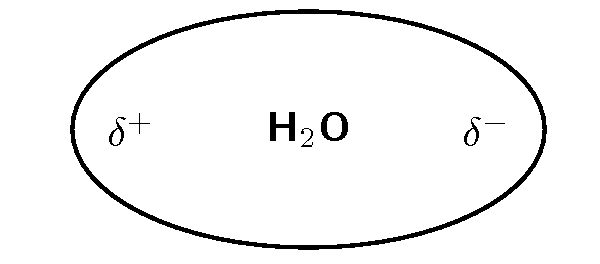
\includegraphics[width=5cm]{col11305.imgs/m38720_CG10C8_001.png} % m38720;CG10C8\_001.png;;;6.0;8.5;
        
      \vspace{2pt}
    \vspace{\rubberspace}\par \begin{cnxcaption}
	  \small \textbf{Figure 17.1: }Water is a polar molecule
	\end{cnxcaption}
      
    \vspace{.1in}
    \rule[.1in]{\figurerulewidth}{.005in} \\
        
    \end{center}

 \end{figure}   

    \addtocounter{footnote}{-0}
    
        \label{m38720*id335349}It is the polar nature of water that allows ionic compounds to dissolve in it. In the case of sodium chloride (\begin{math}\mathrm{NaCl}\end{math}) for example, the positive sodium ions (\begin{math}{\mathrm{Na}}^{+}\end{math}) will be attracted to the negative pole of the water molecule, while the negative chloride ions (\begin{math}{\mathrm{Cl}}^{-}\end{math}) will be attracted to the positive pole of the water molecule. In the process, the ionic bonds between the sodium and chloride ions are weakened and the water molecules are able to work their way between the individual ions, surrounding them and slowly dissolving the compound. This process is called \textbf{dissociation}. A simplified representation of this is shown in Figure~17.2. We say that dissolution of a substance has occurred when a substance dissociates or dissolves.\par 
\label{m38720*fhsst!!!underscore!!!id155}\begin{definition}
	  \begin{tabular*}{15 cm}{m{15 mm}m{}}
	\hspace*{-50pt}  
\includegraphics[width=0.5in]{col11305.imgs/psflag2.png}   & \Definition{   \label{id2490327}\textbf{ Dissociation }} { \label{m38720*meaningfhsst!!!underscore!!!id155}
        Dissociation in chemistry and biochemistry is a general process in which ionic compounds separate or split into smaller molecules or ions, usually in a reversible manner.  
         } 
      \end{tabular*}
      \end{definition}

        
    \setcounter{subfigure}{0}


	\begin{figure}[H] % horizontal\label{m38720*uid21}
    \begin{center}
    \rule[.1in]{\figurerulewidth}{.005in} \\
        \label{m38720*uid21!!!underscore!!!media}\label{m38720*uid21!!!underscore!!!printimage}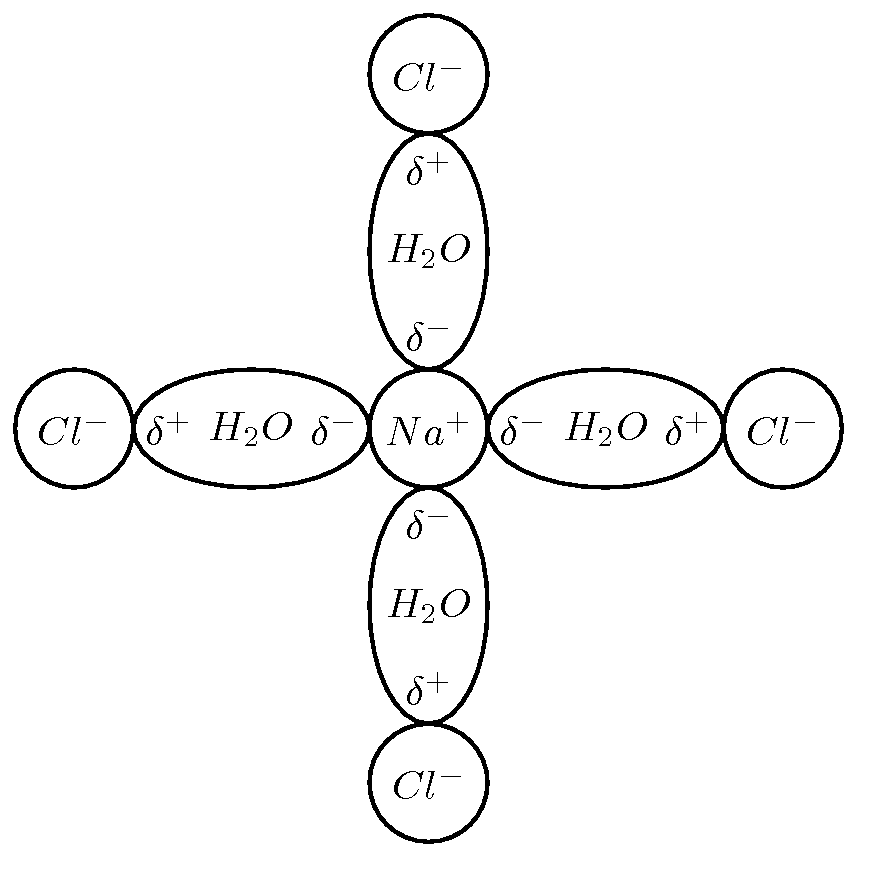
\includegraphics{col11305.imgs/m38720_CG10C8_002.png} % m38720;CG10C8\_002.png;;;6.0;8.5;
        
      \vspace{2pt}
    \vspace{\rubberspace}\par \begin{cnxcaption}
	  \small \textbf{Figure 17.2: }Sodium chloride dissolves in water
	\end{cnxcaption}
      
    \vspace{.1in}
    \rule[.1in]{\figurerulewidth}{.005in} \\
        
    \end{center}

 \end{figure}   

    \addtocounter{footnote}{-0}
    
        \label{m38720*id335421}The dissolution of sodium chloride can be represented by the following equation:\par 
        \label{m38720*uid3241}\begin{math}\mathrm{NaCl\left(s\right)}\to {\mathrm{Na}}^{+}\mathrm{\left(aq\right)}+{\mathrm{Cl}}^{-}\mathrm{\left(aq\right)}\end{math}
        \par 
        \label{m38720*id333999}The symbols \textbf{s} (solid), \textbf{l} (liquid), \textbf{g} (gas) and \textbf{aq} (material is dissolved in water) are written after the chemical formula to show the state or phase of the material. The dissolution of potassium sulphate into potassium and sulphate ions is shown below as another example:\par 
        \label{m38720*uid971321}\begin{math}{\mathrm{K}}_{2}{\mathrm{SO}}_{4}\mathrm{\left(s\right)}\to 2{\mathrm{K}}^{+}\mathrm{\left(aq\right)}+\mathrm{SO}_{4}^{2-}\mathrm{\left(aq\right)}\end{math}
        \par 
        \label{m38720*id335781}Remember that \textbf{molecular} substances (e.g. covalent compounds) may also dissolve, but most will not form ions. One example is sugar.\par 
        \label{m38720*uid922381}\begin{math}{\mathrm{C}}_{6}{\mathrm{H}}_{12}{\mathrm{O}}_{6}\mathrm{\left(s\right)}⇌{\mathrm{C}}_{6}{\mathrm{H}}_{12}{\mathrm{O}}_{6}\mathrm{\left(aq\right)}\end{math}
        \par 
        \label{m38720*id335863}There are exceptions to this and some molecular substances \textsl{will} form ions when they dissolve. Hydrogen chloride for example can ionise to form hydrogen and chloride ions.\par 
        \label{m38720*uid98732}\begin{math}\mathrm{HCl\left(g\right)}\to {\mathrm{H}}^{+}\mathrm{\left(aq\right)}+{\mathrm{Cl}}^{-}\mathrm{\left(aq\right)}\end{math}
        \par 

\par
            \label{m38720*eip-687}\vspace{.5cm} 
      
      \noindent
      \hspace*{-30pt}
\includegraphics[width=0.5in]{col11305.imgs/pspencil2.png}   \raisebox{25mm}{   
      \begin{mdframed}[linewidth=4, leftmargin=40, rightmargin=40]  
      \begin{exercise}
    \noindent\textbf{Exercise 17.1: Dissociation in water}\label{m38720*eip-470}
  \label{m38720*eip-646}
    Write a balanced equation to show how silver nitrate (\begin{math}{\mathrm{AgNO}}_{3}\end{math}) dissociates in water.
  \par 
\vspace{5pt}

\label{m38720*eip-172}\noindent\textbf{Solution to Exercise }
\label{m38720*id7534}\begin{enumerate}[noitemsep, label=\textbf{Step} \textbf{\arabic*}. ] 
            \leftskip=20pt\rightskip=\leftskip\item The cation is: \begin{math}{Ag}^{+}\end{math} and the anion is: \begin{math}\mathrm{NO}_{3}^{-}\end{math}\item Since we know both the anion and the cation that silver nitrate dissociates into we can write the following equation:
\label{m38720*id843}\nopagebreak\noindent{}\settowidth{\mymathboxwidth}{\begin{equation}
    {\mathrm{AgNO}}_{3}\mathrm{\left(s\right)}\to {Ag}^{+}\mathrm{\left(aq\right)}+\mathrm{NO}_{3}^{-}\mathrm{\left(aq\right)}\tag{17.1}
      \end{equation}
    }
    \typeout{Columnwidth = \the\columnwidth}\typeout{math as usual width = \the\mymathboxwidth}
    \ifthenelse{\lengthtest{\mymathboxwidth < \columnwidth}}{% if the math fits, do it again, for real
    \begin{equation}
    {\mathrm{AgNO}}_{3}\mathrm{\left(s\right)}\to {Ag}^{+}\mathrm{\left(aq\right)}+\mathrm{NO}_{3}^{-}\mathrm{\left(aq\right)}\tag{17.1}
      \end{equation}
    }{% else, if it doesn't fit
    \setlength{\mymathboxwidth}{\columnwidth}
      \addtolength{\mymathboxwidth}{-48pt}
    \par\vspace{12pt}\noindent\begin{minipage}{\columnwidth}
    \parbox[t]{\mymathboxwidth}{\large\begin{math}
    {\mathrm{AgNO}}_{3}\mathrm{\left(s\right)}\to {Ag}^{+}\mathrm{\left(aq\right)}+\mathrm{NO}_{3}^{-}\mathrm{\left(aq\right)}\end{math}}\hfill
    \parbox[t]{48pt}{\raggedleft 
    (17.1)}
    \end{minipage}\vspace{12pt}\par
    }% end of conditional for this bit of math
    \typeout{math as usual width = \the\mymathboxwidth}
    
\end{enumerate}
        


    \end{exercise}
    \end{mdframed}
    }
    \noindent
  \label{m38720*secfhsst!!!underscore!!!id338}
            \subsubsection{ Ions in solution         }
            \nopagebreak
            \label{m38720*id336094}\begin{enumerate}[noitemsep, label=\textbf{\arabic*}. ] 
            \label{m38720*uid22}\item For each of the following, say whether the substance is ionic or molecular.
\label{m38720*id336110}\begin{enumerate}[noitemsep, label=\textbf{\alph*}. ] 
            \label{m38720*uid23}\item potassium nitrate (\begin{math}\mathrm{KNO}{}_{3}\end{math})
\label{m38720*uid24}\item ethanol (\begin{math}\mathrm{C}{}_{2}\mathrm{H}{}_{5}\mathrm{OH}\end{math})
\label{m38720*uid25}\item sucrose (a type of sugar) (\begin{math}\mathrm{C}{}_{12}\mathrm{H}{}_{22}\mathrm{O}{}_{11}\end{math})\label{m38720*uid26}\item sodium bromide (\begin{math}\mathrm{NaBr}\end{math})
\end{enumerate}
                

\label{m38720*uid27}\item Write a balanced equation to show how each of the following ionic compounds dissociate in water.
\label{m38720*id336252}\begin{enumerate}[noitemsep, label=\textbf{\alph*}. ] 
            \label{m38720*uid28}\item sodium sulphate (\begin{math}\mathrm{Na}{}_{2}\mathrm{SO}{}_{4}\end{math})
\label{m38720*uid29}\item potassium bromide (\begin{math}\mathrm{KBr}\end{math})
\label{m38720*uid30}\item potassium permanganate (\begin{math}\mathrm{KMnO}{}_{4}\end{math})
\label{m38720*uid31}\item sodium phosphate (\begin{math}\mathrm{Na}{}_{3}\mathrm{PO}{}_{4}\end{math})
\end{enumerate}
                
\end{enumerate}
        
        

      
      \label{m38720*uid32}
\par \raisebox{-5 pt}{
\includegraphics[width=0.5cm]{col11305.imgs/summary_www.png}} Find the answers with the shortcodes:
 \par \begin{tabular}[h]{cccccc}
 (1.) l33  &  (2.) l3g  & \end{tabular}



            \subsubsection{ Applications}
            \nopagebreak
            \label{m38720*eip-id1165497780773}\begin{enumerate}[noitemsep, label=\textbf{\arabic*}. ] 
            \item 
\par
            \label{m38720*fhsst!!!underscore!!!id358}\begin{definition}
	  \begin{tabular*}{15 cm}{m{15 mm}m{}}
	\hspace*{-50pt}  
\includegraphics[width=0.5in]{col11305.imgs/psflag2.png}   & \Definition{   \label{id2491081}\textbf{ Water hardness }} { \label{m38720*meaningfhsst!!!underscore!!!id358}
        Water hardness is a measure of the mineral content of water. Minerals are substances such as calcite, quartz and mica that occur naturally as a result of geological processes. 
         } 
      \end{tabular*}
      \end{definition}

        \label{m38720*id336408}\textbf{Hard water} is water that has a high mineral content. Water that has a low mineral content is known as \textbf{soft water}. If water has a high mineral content, it usually contains high levels of metal ions, mainly calcium (\begin{math}\mathrm{Ca}\end{math}) and magnesium (\begin{math}\mathrm{Mg}\end{math}). The calcium enters the water from either \begin{math}{\mathrm{CaCO}}_{3}\end{math} (limestone or chalk) or from mineral deposits of \begin{math}{\mathrm{CaSO}}_{4}\end{math}. The main source of magnesium is a sedimentary rock called dolomite, \begin{math}{\mathrm{CaMg\left(CO}}_{3}\mathrm{\right)}{}_{2}\end{math}. Hard water may also contain other metals as well as bicarbonates and sulphates.\par 
\label{m38720*notfhsst!!!underscore!!!id362}
\begin{tabular}{cc}
	\hspace*{-50pt}\raisebox{-8 mm}{\hspace{-0.2in}
\includegraphics[width=0.75in]{col11305.imgs/psfact2.png} } & 

	\begin{minipage}{0.85\textwidth}
	\begin{note}
      {note: } The simplest way to check whether water is hard or soft is to use the lather/froth test. If the water is very soft, soap will lather more easily when it is rubbed against the skin. With hard water this won't happen. Toothpaste will also not froth well in hard water.
	\end{note}
	\end{minipage}
	\end{tabular}
	\par
      
        \label{m38720*id336486}A \textbf{water softener} works on the principle of \textbf{ion exchange}. Hard water passes through a media bed, usually made of resin beads that are supersaturated with sodium. As the water passes through the beads, the hardness minerals (e.g. calcium and magnesium) attach themselves to the beads. The sodium that was originally on the beads is released into the water. When the resin becomes saturated with calcium and magnesium, it must be recharged. A salt solution is passed through the resin. The sodium replaces the calcium and magnesium and these ions are released into the waste water and discharged.\par \item \label{m38720*eip-id1164949856187}The acidity of rainwater comes from the natural presence of three substances (\begin{math}\mathrm{CO}{}_{2}\end{math}, \begin{math}\mathrm{NO}\end{math}, and \begin{math}\mathrm{SO}{}_{2}\end{math}) in the lowest layer of the atmosphere. These gases are able to dissolve in water and therefore make rain more acidic than it would otherwise be. Of these gases, carbon dioxide (\begin{math}\mathrm{CO}{}_{2}\end{math}) has the highest concentration and therefore contributes the most to the natural acidity of rainwater. \par 
\label{m38720*fhsst!!!underscore!!!id5341}\begin{definition}
	  \begin{tabular*}{15 cm}{m{15 mm}m{}}
	\hspace*{-50pt}  
\includegraphics[width=0.5in]{col11305.imgs/psflag2.png}   & \Definition{   \label{id2491282}\textbf{ Acid rain }} { \label{m38720*meaningfhsst!!!underscore!!!id5341}
       Acid rain refers to the deposition of acidic components in rain, snow and dew. Acid rain occurs when sulphur dioxide and nitrogen oxides are emitted into the atmosphere, undergo chemical transformations and are absorbed by water droplets in clouds. The droplets then fall to earth as rain, snow, mist, dry dust, hail, or sleet. This increases the acidity of the soil and affects the chemical balance of lakes and streams. 
         } 
      \end{tabular*}
      \end{definition}

\label{m38720*id338300}Although these reactions do take place naturally, human activities can greatly increase the concentration of these gases in the atmosphere, so that rain becomes far more acidic than it would otherwise be. The burning of fossil fuels in industries, vehicles etc is one of the biggest culprits. If the acidity of the rain drops to below 5, it is referred to as \textbf{acid rain}.\par 
        \label{m38720*id338311}Acid rain can have a very damaging effect on the environment. In rivers, dams and lakes, increased acidity can mean that some species of animals and plants will not survive. Acid rain can also degrade soil minerals, producing metal ions that are washed into water systems. Some of these ions may be toxic e.g. \begin{math}{\mathrm{Al}}^{3+}\end{math}. From an economic perspective, altered soil pH can drastically affect agricultural productivity.\par 
        \label{m38720*id338337}Acid rain can also affect buildings and monuments, many of which are made from marble and limestone. A chemical reaction takes place between \begin{math}{\mathrm{CaCO}}_{3}\end{math} (limestone) and sulphuric acid to produce aqueous ions which can be easily washed away. The same reaction can occur in the lithosphere where limestone rocks are present e.g. limestone caves can be eroded by acidic rainwater.
        \label{m38720*id7435}\nopagebreak\noindent{}
        \settowidth{\mymathboxwidth}{\begin{equation}
    {\mathrm{H}}_{2}{\mathrm{SO}}_{4}+{\mathrm{CaCO}}_{3}\to {\mathrm{CaSO}}_{4}\ensuremath{\cdot}\mathrm{H}{}_{2}\mathrm{O}+{\mathrm{CO}}_{2}\tag{17.2}
      \end{equation}
    }
    \typeout{Columnwidth = \the\columnwidth}\typeout{math as usual width = \the\mymathboxwidth}
    \ifthenelse{\lengthtest{\mymathboxwidth < \columnwidth}}{% if the math fits, do it again, for real
    \begin{equation}
    {\mathrm{H}}_{2}{\mathrm{SO}}_{4}+{\mathrm{CaCO}}_{3}\to {\mathrm{CaSO}}_{4}\ensuremath{\cdot}\mathrm{H}{}_{2}\mathrm{O}+{\mathrm{CO}}_{2}\tag{17.2}
      \end{equation}
    }{% else, if it doesn't fit
    \setlength{\mymathboxwidth}{\columnwidth}
      \addtolength{\mymathboxwidth}{-48pt}
    \par\vspace{12pt}\noindent\begin{minipage}{\columnwidth}
    \parbox[t]{\mymathboxwidth}{\large\begin{math}
    {\mathrm{H}}_{2}{\mathrm{SO}}_{4}+{\mathrm{CaCO}}_{3}\to {\mathrm{CaSO}}_{4}\ensuremath{\cdot}\mathrm{H}{}_{2}\mathrm{O}+{\mathrm{CO}}_{2}\end{math}}\hfill
    \parbox[t]{48pt}{\raggedleft 
    (17.2)}
    \end{minipage}\vspace{12pt}\par
    }% end of conditional for this bit of math
    \typeout{math as usual width = \the\mymathboxwidth}
    

\par 
\end{enumerate}
            
      
      
    
 
    \label{m38720*cid7}
            \subsection{ Electrolytes, ionisation and conductivity}
            \nopagebreak
            
      
      \label{m38720*id338608}\textbf{Conductivity} in aqueous solutions, is a measure of the ability of water to conduct an electric current. The more \textbf{ions} there are in the solution, the higher its conductivity.\par 
\label{m38720*fhsst!!!underscore!!!id635}\begin{definition}
	  \begin{tabular*}{15 cm}{m{15 mm}m{}}
	\hspace*{-50pt}  
\includegraphics[width=0.5in]{col11305.imgs/psflag2.png}   & \Definition{   \label{id2491504}\textbf{ Conductivity }} { \label{m38720*meaningfhsst!!!underscore!!!id635}
      Conductivity is a measure of a solution's ability to conduct an electric current.
       } 
      \end{tabular*}
      \end{definition}

      \label{m38720*uid52}
            \subsubsection{ Electrolytes}
            \nopagebreak
            
        
        \label{m38720*id338650}An \textbf{electrolyte} is a material that \textsl{increases} the conductivity of water when dissolved in it. Electrolytes can be further divided into \textbf{strong electrolytes} and \textbf{weak electrolytes}.\par 
\label{m38720*fhsst!!!underscore!!!id641}\begin{definition}
	  \begin{tabular*}{15 cm}{m{15 mm}m{}}
	\hspace*{-50pt}  
\includegraphics[width=0.5in]{col11305.imgs/psflag2.png}   & \Definition{   \label{id2491564}\textbf{ Electrolyte }} { \label{m38720*meaningfhsst!!!underscore!!!id641}
        An electrolyte is a substance that contains free ions and behaves as an electrically conductive medium. Because they generally consist of ions in solution, electrolytes are also known as ionic solutions. 
         } 
      \end{tabular*}
      \end{definition}

        \label{m38720*id338697}\begin{enumerate}[noitemsep, label=\textbf{\arabic*}. ] 
            \label{m38720*uid53}\item \textbf{Strong electrolytes}
A strong electrolyte is a material that ionises completely when it is dissolved in water:
\label{m38720*id338720}\nopagebreak\noindent{}\settowidth{\mymathboxwidth}{\begin{equation}
    \mathrm{AB\; \left(s,\; l,\; g\right)}\to {\mathrm{A}}^{+}\mathrm{\left(aq\right)}+{\mathrm{B}}^{-}\mathrm{\left(aq\right)}\tag{17.3}
      \end{equation}
    }
    \typeout{Columnwidth = \the\columnwidth}\typeout{math as usual width = \the\mymathboxwidth}
    \ifthenelse{\lengthtest{\mymathboxwidth < \columnwidth}}{% if the math fits, do it again, for real
    \begin{equation}
    \mathrm{AB\; \left(s,\; l,\; g\right)}\to {\mathrm{A}}^{+}\mathrm{\left(aq\right)}+{\mathrm{B}}^{-}\mathrm{\left(aq\right)}\tag{17.3}
      \end{equation}
    }{% else, if it doesn't fit
    \setlength{\mymathboxwidth}{\columnwidth}
      \addtolength{\mymathboxwidth}{-48pt}
    \par\vspace{12pt}\noindent\begin{minipage}{\columnwidth}
    \parbox[t]{\mymathboxwidth}{\large\begin{math}
    \mathrm{AB\; \left(s,\; l,\; g\right)}\to {\mathrm{A}}^{+}\mathrm{\left(aq\right)}+{\mathrm{B}}^{-}\mathrm{\left(aq\right)}\end{math}}\hfill
    \parbox[t]{48pt}{\raggedleft 
    (17.3)}
    \end{minipage}\vspace{12pt}\par
    }% end of conditional for this bit of math
    \typeout{math as usual width = \the\mymathboxwidth}
    
This is a \textbf{chemical change} because the original compound has been split into its component ions and bonds have been broken. In a strong electrolyte, we say that the \textsl{extent of ionisation} is high. In other words, the original material dissociates completely so that there is a high concentration of ions in the solution. An example is a solution of potassium nitrate:
\label{m38720*id338807}\nopagebreak\noindent{}\settowidth{\mymathboxwidth}{\begin{equation}
    {\mathrm{KNO}}_{3}\mathrm{\left(s\right)}\to {\mathrm{K}}^{+}\mathrm{\left(aq\right)}+\mathrm{NO}_{3}^{-}\mathrm{\left(aq\right)}\tag{17.4}
      \end{equation}
    }
    \typeout{Columnwidth = \the\columnwidth}\typeout{math as usual width = \the\mymathboxwidth}
    \ifthenelse{\lengthtest{\mymathboxwidth < \columnwidth}}{% if the math fits, do it again, for real
    \begin{equation}
    {\mathrm{KNO}}_{3}\mathrm{\left(s\right)}\to {\mathrm{K}}^{+}\mathrm{\left(aq\right)}+\mathrm{NO}_{3}^{-}\mathrm{\left(aq\right)}\tag{17.4}
      \end{equation}
    }{% else, if it doesn't fit
    \setlength{\mymathboxwidth}{\columnwidth}
      \addtolength{\mymathboxwidth}{-48pt}
    \par\vspace{12pt}\noindent\begin{minipage}{\columnwidth}
    \parbox[t]{\mymathboxwidth}{\large\begin{math}
    {\mathrm{KNO}}_{3}\mathrm{\left(s\right)}\to {\mathrm{K}}^{+}\mathrm{\left(aq\right)}+\mathrm{NO}_{3}^{-}\mathrm{\left(aq\right)}\end{math}}\hfill
    \parbox[t]{48pt}{\raggedleft 
    (17.4)}
    \end{minipage}\vspace{12pt}\par
    }% end of conditional for this bit of math
    \typeout{math as usual width = \the\mymathboxwidth}
    \label{m38720*uid54}\item \textbf{Weak electrolytes}
A weak electrolyte is a material that goes into solution and will be surrounded by water molecules when it is added to water. However, not \textsl{all} of the molecules will dissociate into ions. The \textsl{extent of ionisation} of a weak electrolyte is low and therefore the concentration of ions in the solution is also low.
\label{m38720*id338913}\nopagebreak\noindent{}\settowidth{\mymathboxwidth}{\begin{equation}
    AB\left(s,l,g\right)\to AB\left(aq\right)⇌{A}^{+}\left(\mathrm{aq}\right)+{B}^{-}\left(\mathrm{aq}\right)\tag{17.5}
      \end{equation}
    }
    \typeout{Columnwidth = \the\columnwidth}\typeout{math as usual width = \the\mymathboxwidth}
    \ifthenelse{\lengthtest{\mymathboxwidth < \columnwidth}}{% if the math fits, do it again, for real
    \begin{equation}
    AB\left(s,l,g\right)\to AB\left(aq\right)⇌{A}^{+}\left(\mathrm{aq}\right)+{B}^{-}\left(\mathrm{aq}\right)\tag{17.5}
      \end{equation}
    }{% else, if it doesn't fit
    \setlength{\mymathboxwidth}{\columnwidth}
      \addtolength{\mymathboxwidth}{-48pt}
    \par\vspace{12pt}\noindent\begin{minipage}{\columnwidth}
    \parbox[t]{\mymathboxwidth}{\large\begin{math}
    AB\left(s,l,g\right)\to AB\left(aq\right)⇌{A}^{+}\left(\mathrm{aq}\right)+{B}^{-}\left(\mathrm{aq}\right)\end{math}}\hfill
    \parbox[t]{48pt}{\raggedleft 
    (17.5)}
    \end{minipage}\vspace{12pt}\par
    }% end of conditional for this bit of math
    \typeout{math as usual width = \the\mymathboxwidth}
    
The following example shows that in the final solution of a weak electrolyte, some of the original compound \textsl{plus} some dissolved ions are present.
\label{m38720*id339008}\nopagebreak\noindent{}\settowidth{\mymathboxwidth}{\begin{equation}
    {C}_{2}{H}_{3}{O}_{2}H\left(l\right)\to {C}_{2}{H}_{3}{O}_{2}H⇌{C}_{2}{H}_{3}O_{2}^{-}\left(\mathrm{aq}\right)+{H}^{+}\left(\mathrm{aq}\right)\tag{17.6}
      \end{equation}
    }
    \typeout{Columnwidth = \the\columnwidth}\typeout{math as usual width = \the\mymathboxwidth}
    \ifthenelse{\lengthtest{\mymathboxwidth < \columnwidth}}{% if the math fits, do it again, for real
    \begin{equation}
    {C}_{2}{H}_{3}{O}_{2}H\left(l\right)\to {C}_{2}{H}_{3}{O}_{2}H⇌{C}_{2}{H}_{3}O_{2}^{-}\left(\mathrm{aq}\right)+{H}^{+}\left(\mathrm{aq}\right)\tag{17.6}
      \end{equation}
    }{% else, if it doesn't fit
    \setlength{\mymathboxwidth}{\columnwidth}
      \addtolength{\mymathboxwidth}{-48pt}
    \par\vspace{12pt}\noindent\begin{minipage}{\columnwidth}
    \parbox[t]{\mymathboxwidth}{\large\begin{math}
    {C}_{2}{H}_{3}{O}_{2}H\left(l\right)\to {C}_{2}{H}_{3}{O}_{2}H⇌{C}_{2}{H}_{3}O_{2}^{-}\left(\mathrm{aq}\right)+{H}^{+}\left(\mathrm{aq}\right)\end{math}}\hfill
    \parbox[t]{48pt}{\raggedleft 
    (17.6)}
    \end{minipage}\vspace{12pt}\par
    }% end of conditional for this bit of math
    \typeout{math as usual width = \the\mymathboxwidth}
    \end{enumerate}
        
      
      \label{m38720*uid55}
            \subsubsection{ Non-electrolytes}
            \nopagebreak
            
        
        \label{m38720*id339146}A \textbf{non-electrolyte} is a material that does not increase the conductivity of water when dissolved in it. The substance goes into solution and becomes surrounded by water molecules, so that the molecules of the chemical become separated from each other. However, although the substance does dissolve, it is not changed in any way and no chemical bonds are broken. The change is a \textbf{physical change}. In the oxygen example below, the reaction is shown to be reversible because oxygen is only partially soluble in water and comes out of solution very easily.\par 
        \label{m38720*id339165}\nopagebreak\noindent{}
          \settowidth{\mymathboxwidth}{\begin{equation}
    {C}_{2}{H}_{5}\mathrm{OH}\left(l\right)\to {C}_{2}{H}_{5}\mathrm{OH}\left(\mathrm{aq}\right)\tag{17.7}
      \end{equation}
    }
    \typeout{Columnwidth = \the\columnwidth}\typeout{math as usual width = \the\mymathboxwidth}
    \ifthenelse{\lengthtest{\mymathboxwidth < \columnwidth}}{% if the math fits, do it again, for real
    \begin{equation}
    {C}_{2}{H}_{5}\mathrm{OH}\left(l\right)\to {C}_{2}{H}_{5}\mathrm{OH}\left(\mathrm{aq}\right)\tag{17.7}
      \end{equation}
    }{% else, if it doesn't fit
    \setlength{\mymathboxwidth}{\columnwidth}
      \addtolength{\mymathboxwidth}{-48pt}
    \par\vspace{12pt}\noindent\begin{minipage}{\columnwidth}
    \parbox[t]{\mymathboxwidth}{\large\begin{math}
    {C}_{2}{H}_{5}\mathrm{OH}\left(l\right)\to {C}_{2}{H}_{5}\mathrm{OH}\left(\mathrm{aq}\right)\end{math}}\hfill
    \parbox[t]{48pt}{\raggedleft 
    (17.7)}
    \end{minipage}\vspace{12pt}\par
    }% end of conditional for this bit of math
    \typeout{math as usual width = \the\mymathboxwidth}
    
        
        \label{m38720*id339233}\nopagebreak\noindent{}
          \settowidth{\mymathboxwidth}{\begin{equation}
    {O}_{2}\left(g\right)⇌{O}_{2}\left(\mathrm{aq}\right)\tag{17.8}
      \end{equation}
    }
    \typeout{Columnwidth = \the\columnwidth}\typeout{math as usual width = \the\mymathboxwidth}
    \ifthenelse{\lengthtest{\mymathboxwidth < \columnwidth}}{% if the math fits, do it again, for real
    \begin{equation}
    {O}_{2}\left(g\right)⇌{O}_{2}\left(\mathrm{aq}\right)\tag{17.8}
      \end{equation}
    }{% else, if it doesn't fit
    \setlength{\mymathboxwidth}{\columnwidth}
      \addtolength{\mymathboxwidth}{-48pt}
    \par\vspace{12pt}\noindent\begin{minipage}{\columnwidth}
    \parbox[t]{\mymathboxwidth}{\large\begin{math}
    {O}_{2}\left(g\right)⇌{O}_{2}\left(\mathrm{aq}\right)\end{math}}\hfill
    \parbox[t]{48pt}{\raggedleft 
    (17.8)}
    \end{minipage}\vspace{12pt}\par
    }% end of conditional for this bit of math
    \typeout{math as usual width = \the\mymathboxwidth}
    
        
      
      \label{m38720*uid56}
            \subsubsection{ Factors that affect the conductivity of water}
            \nopagebreak
            \label{m38720*id339287}The conductivity of water is therefore affected by the following factors:\par 
        \label{m38720*id339291}\begin{itemize}[noitemsep]
            \label{m38720*uid57}\item The \textbf{type of substance} that dissolves in water.
Whether a material is a strong electrolyte (e.g. potassium nitrate, \begin{math}{\mathrm{KNO}}_{3}\end{math}), a weak electrolyte (e.g. acetate, \begin{math}{\mathrm{CH}}_{3}\mathrm{COOH}\end{math}) or a non-electrolyte (e.g. sugar, alcohol, oil) will affect the conductivity of water because the concentration of ions in solution will be different in each case.
\label{m38720*uid58}\item The \textbf{concentration of ions} in solution.
The higher the concentration of ions in solution, the higher its conductivity will be.
\label{m38720*uid59}\item \textbf{Temperature.}
The warmer the solution, the higher the solubility of the material being dissolved and therefore the higher the conductivity as well.
\end{itemize}
        
\label{m38720*secfhsst!!!underscore!!!id739}
            \subsubsection{ Experiment : Electrical conductivity         }
            \nopagebreak
            \label{m38720*id339425}\noindent{}\textbf{Aim:}
          \newline
    
To investigate the electrical conductivities of different substances and solutions.\par 
        \label{m38720*id339438}\noindent{}\textbf{Apparatus:}
          \newline
    
        Solid salt (\begin{math}\mathrm{NaCl}\end{math}) crystals; different liquids such as distilled water, tap water, seawater, benzene and alcohol; solutions of salts e.g. \begin{math}\mathrm{NaCl}\end{math}, \begin{math}\mathrm{KBr}\end{math}; a solution of an acid (e.g. \begin{math}\mathrm{HCl}\end{math}) and a solution of a base (e.g. \begin{math}\mathrm{NaOH}\end{math}); torch cells; ammeter; conducting wire, crocodile clips and 2 carbon rods.\par 
        \label{m38720*eip-456}
\begin{tabular}{cc}
	\hspace*{-50pt}\raisebox{-8 mm}{\hspace{-0.2in}
\includegraphics[width=0.5in]{col11305.imgs/pstip2.png} } & 

	\begin{minipage}{0.85\textwidth}
	\begin{note}
      {warning: }Always use benzene in a fume cupboard as it is very toxic. If you don't have access to a fume cupboard then ensure that the work area is well ventilated. 
	\end{note}
	\end{minipage}
	\end{tabular}
	\par
      \label{m38720*id334346}\noindent{}\textbf{Method:}
          \newline
    
        Set up the experiment by connecting the circuit as shown in the diagram below. In the diagram, 'X' represents the substance or solution that you will be testing. When you are using the solid crystals, the crocodile clips can be attached directly to each end of the crystal. When you are using solutions, two carbon rods are placed into the liquid and the clips are attached to each of the rods. In each case, complete the circuit and allow the current to flow for about 30 seconds. Observe whether the ammeter shows a reading.\par 
        \label{m38720*id334362}
          
    \setcounter{subfigure}{0}


	\begin{figure}[H] % horizontal\label{m38720*id334366}
    \begin{center}
    \label{m38720*id334366!!!underscore!!!media}\label{m38720*id334366!!!underscore!!!printimage}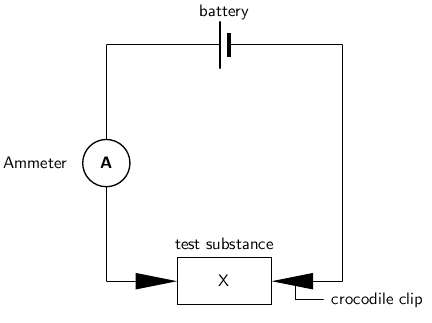
\includegraphics[width=7cm]{col11305.imgs/m38720_CG10C8_003.png} % m38720;CG10C8\_003.png;;;6.0;8.5;
        
      \vspace{2pt}
    \vspace{.1in}
    
    \end{center}

 \end{figure}   

    \addtocounter{footnote}{-0}
    
        \par 
        \label{m38720*id334372}\noindent{}\textbf{Results:}
          \newline
    
        Record your observations in a table similar to the one below:
        
    % \textbf{m38720*id334385}\par
    
    % how many colspecs?  2
          % name: cnx:colspec
            % colnum: 1
            % colwidth: 10*
            % latex-name: columna
            % colname: 
            % align/tgroup-align/default: //left
            % -------------------------
            % name: cnx:colspec
            % colnum: 2
            % colwidth: 10*
            % latex-name: columnb
            % colname: 
            % align/tgroup-align/default: //left
            % -------------------------
      
    
    \setlength\mytablespace{4\tabcolsep}
    \addtolength\mytablespace{3\arrayrulewidth}
    \setlength\mytablewidth{\linewidth}
        
    
    \setlength\mytableroom{\mytablewidth}
    \addtolength\mytableroom{-\mytablespace}
    
    \setlength\myfixedwidth{0pt}
    \setlength\mystarwidth{\mytableroom}
        \addtolength\mystarwidth{-\myfixedwidth}
        \divide\mystarwidth 20
        
    
      % ----- Begin capturing width of table in LR mode woof
      \settowidth{\mytableboxwidth}{\begin{tabular}[t]{|l|l|}\hline
    % count in rowspan-info-nodeset: 2
    % align/colidx: left,1
    
    % rowcount: '0' | start: 'false' | colidx: '1'
    
        % Formatting a regular cell and recurring on the next sibling
        Test substance &
      % align/colidx: left,2
    
    % rowcount: '0' | start: 'false' | colidx: '2'
    
        % Formatting a regular cell and recurring on the next sibling
        Ammeter reading% make-rowspan-placeholders
    % rowspan info: col1 '0' | 'false' | '' || col2 '0' | 'false' | ''
     \tabularnewline\cline{1-1}\cline{2-2}
      %--------------------------------------------------------------------
    % align/colidx: left,1
    
    % rowcount: '0' | start: 'false' | colidx: '1'
    
        % Formatting a regular cell and recurring on the next sibling
         &
      % align/colidx: left,2
    
    % rowcount: '0' | start: 'false' | colidx: '2'
    
        % Formatting a regular cell and recurring on the next sibling
        % make-rowspan-placeholders
    % rowspan info: col1 '0' | 'false' | '' || col2 '0' | 'false' | ''
     \tabularnewline\cline{1-1}\cline{2-2}
      %--------------------------------------------------------------------
    % align/colidx: left,1
    
    % rowcount: '0' | start: 'false' | colidx: '1'
    
        % Formatting a regular cell and recurring on the next sibling
         &
      % align/colidx: left,2
    
    % rowcount: '0' | start: 'false' | colidx: '2'
    
        % Formatting a regular cell and recurring on the next sibling
        % make-rowspan-placeholders
    % rowspan info: col1 '0' | 'false' | '' || col2 '0' | 'false' | ''
     \tabularnewline\cline{1-1}\cline{2-2}
      %--------------------------------------------------------------------
    % align/colidx: left,1
    
    % rowcount: '0' | start: 'false' | colidx: '1'
    
        % Formatting a regular cell and recurring on the next sibling
         &
      % align/colidx: left,2
    
    % rowcount: '0' | start: 'false' | colidx: '2'
    
        % Formatting a regular cell and recurring on the next sibling
        % make-rowspan-placeholders
    % rowspan info: col1 '0' | 'false' | '' || col2 '0' | 'false' | ''
     \tabularnewline\cline{1-1}\cline{2-2}
      %--------------------------------------------------------------------
    % align/colidx: left,1
    
    % rowcount: '0' | start: 'false' | colidx: '1'
    
        % Formatting a regular cell and recurring on the next sibling
         &
      % align/colidx: left,2
    
    % rowcount: '0' | start: 'false' | colidx: '2'
    
        % Formatting a regular cell and recurring on the next sibling
        % make-rowspan-placeholders
    % rowspan info: col1 '0' | 'false' | '' || col2 '0' | 'false' | ''
     \tabularnewline\cline{1-1}\cline{2-2}
      %--------------------------------------------------------------------
    \end{tabular}} % end mytableboxwidth set
      \addtocounter{footnote}{-0}
      
      % ----- End capturing width of table in LR mode
    
        % ----- LR or paragraph mode: must test
        % ----- Begin capturing height of table
        \settoheight{\mytableboxheight}{\begin{tabular}[t]{|l|l|}\hline
    % count in rowspan-info-nodeset: 2
    % align/colidx: left,1
    
    % rowcount: '0' | start: 'false' | colidx: '1'
    
        % Formatting a regular cell and recurring on the next sibling
        Test substance &
      % align/colidx: left,2
    
    % rowcount: '0' | start: 'false' | colidx: '2'
    
        % Formatting a regular cell and recurring on the next sibling
        Ammeter reading% make-rowspan-placeholders
    % rowspan info: col1 '0' | 'false' | '' || col2 '0' | 'false' | ''
     \tabularnewline\cline{1-1}\cline{2-2}
      %--------------------------------------------------------------------
    % align/colidx: left,1
    
    % rowcount: '0' | start: 'false' | colidx: '1'
    
        % Formatting a regular cell and recurring on the next sibling
         &
      % align/colidx: left,2
    
    % rowcount: '0' | start: 'false' | colidx: '2'
    
        % Formatting a regular cell and recurring on the next sibling
        % make-rowspan-placeholders
    % rowspan info: col1 '0' | 'false' | '' || col2 '0' | 'false' | ''
     \tabularnewline\cline{1-1}\cline{2-2}
      %--------------------------------------------------------------------
    % align/colidx: left,1
    
    % rowcount: '0' | start: 'false' | colidx: '1'
    
        % Formatting a regular cell and recurring on the next sibling
         &
      % align/colidx: left,2
    
    % rowcount: '0' | start: 'false' | colidx: '2'
    
        % Formatting a regular cell and recurring on the next sibling
        % make-rowspan-placeholders
    % rowspan info: col1 '0' | 'false' | '' || col2 '0' | 'false' | ''
     \tabularnewline\cline{1-1}\cline{2-2}
      %--------------------------------------------------------------------
    % align/colidx: left,1
    
    % rowcount: '0' | start: 'false' | colidx: '1'
    
        % Formatting a regular cell and recurring on the next sibling
         &
      % align/colidx: left,2
    
    % rowcount: '0' | start: 'false' | colidx: '2'
    
        % Formatting a regular cell and recurring on the next sibling
        % make-rowspan-placeholders
    % rowspan info: col1 '0' | 'false' | '' || col2 '0' | 'false' | ''
     \tabularnewline\cline{1-1}\cline{2-2}
      %--------------------------------------------------------------------
    % align/colidx: left,1
    
    % rowcount: '0' | start: 'false' | colidx: '1'
    
        % Formatting a regular cell and recurring on the next sibling
         &
      % align/colidx: left,2
    
    % rowcount: '0' | start: 'false' | colidx: '2'
    
        % Formatting a regular cell and recurring on the next sibling
        % make-rowspan-placeholders
    % rowspan info: col1 '0' | 'false' | '' || col2 '0' | 'false' | ''
     \tabularnewline\cline{1-1}\cline{2-2}
      %--------------------------------------------------------------------
    \end{tabular}} % end mytableboxheight set
        \settodepth{\mytableboxdepth}{\begin{tabular}[t]{|l|l|}\hline
    % count in rowspan-info-nodeset: 2
    % align/colidx: left,1
    
    % rowcount: '0' | start: 'false' | colidx: '1'
    
        % Formatting a regular cell and recurring on the next sibling
        Test substance &
      % align/colidx: left,2
    
    % rowcount: '0' | start: 'false' | colidx: '2'
    
        % Formatting a regular cell and recurring on the next sibling
        Ammeter reading% make-rowspan-placeholders
    % rowspan info: col1 '0' | 'false' | '' || col2 '0' | 'false' | ''
     \tabularnewline\cline{1-1}\cline{2-2}
      %--------------------------------------------------------------------
    % align/colidx: left,1
    
    % rowcount: '0' | start: 'false' | colidx: '1'
    
        % Formatting a regular cell and recurring on the next sibling
         &
      % align/colidx: left,2
    
    % rowcount: '0' | start: 'false' | colidx: '2'
    
        % Formatting a regular cell and recurring on the next sibling
        % make-rowspan-placeholders
    % rowspan info: col1 '0' | 'false' | '' || col2 '0' | 'false' | ''
     \tabularnewline\cline{1-1}\cline{2-2}
      %--------------------------------------------------------------------
    % align/colidx: left,1
    
    % rowcount: '0' | start: 'false' | colidx: '1'
    
        % Formatting a regular cell and recurring on the next sibling
         &
      % align/colidx: left,2
    
    % rowcount: '0' | start: 'false' | colidx: '2'
    
        % Formatting a regular cell and recurring on the next sibling
        % make-rowspan-placeholders
    % rowspan info: col1 '0' | 'false' | '' || col2 '0' | 'false' | ''
     \tabularnewline\cline{1-1}\cline{2-2}
      %--------------------------------------------------------------------
    % align/colidx: left,1
    
    % rowcount: '0' | start: 'false' | colidx: '1'
    
        % Formatting a regular cell and recurring on the next sibling
         &
      % align/colidx: left,2
    
    % rowcount: '0' | start: 'false' | colidx: '2'
    
        % Formatting a regular cell and recurring on the next sibling
        % make-rowspan-placeholders
    % rowspan info: col1 '0' | 'false' | '' || col2 '0' | 'false' | ''
     \tabularnewline\cline{1-1}\cline{2-2}
      %--------------------------------------------------------------------
    % align/colidx: left,1
    
    % rowcount: '0' | start: 'false' | colidx: '1'
    
        % Formatting a regular cell and recurring on the next sibling
         &
      % align/colidx: left,2
    
    % rowcount: '0' | start: 'false' | colidx: '2'
    
        % Formatting a regular cell and recurring on the next sibling
        % make-rowspan-placeholders
    % rowspan info: col1 '0' | 'false' | '' || col2 '0' | 'false' | ''
     \tabularnewline\cline{1-1}\cline{2-2}
      %--------------------------------------------------------------------
    \end{tabular}} % end mytableboxdepth set
        \addtolength{\mytableboxheight}{\mytableboxdepth}
        % ----- End capturing height of table
        \addtocounter{footnote}{-0}
        
        \ifthenelse{\mytableboxwidth<\textwidth}{% the table fits in LR mode
          \addtolength{\mytableboxwidth}{-\mytablespace}
          \typeout{textheight: \the\textheight}
          \typeout{mytableboxheight: \the\mytableboxheight}
          \typeout{textwidth: \the\textwidth}
          \typeout{mytableboxwidth: \the\mytableboxwidth}
          \ifthenelse{\mytableboxheight<\textheight}{%
        
    % \begin{table}[H]
    % \\ '' '0'
    
        \begin{center}
      
      \label{m38720*id334385}
      
    \noindent
    \begin{tabular}[t]{|l|l|}\hline
    % count in rowspan-info-nodeset: 2
    % align/colidx: left,1
    
    % rowcount: '0' | start: 'false' | colidx: '1'
    
        % Formatting a regular cell and recurring on the next sibling
        Test substance &
      % align/colidx: left,2
    
    % rowcount: '0' | start: 'false' | colidx: '2'
    
        % Formatting a regular cell and recurring on the next sibling
        Ammeter reading% make-rowspan-placeholders
    % rowspan info: col1 '0' | 'false' | '' || col2 '0' | 'false' | ''
     \tabularnewline\cline{1-1}\cline{2-2}
      %--------------------------------------------------------------------
    % align/colidx: left,1
    
    % rowcount: '0' | start: 'false' | colidx: '1'
    
        % Formatting a regular cell and recurring on the next sibling
         &
      % align/colidx: left,2
    
    % rowcount: '0' | start: 'false' | colidx: '2'
    
        % Formatting a regular cell and recurring on the next sibling
        % make-rowspan-placeholders
    % rowspan info: col1 '0' | 'false' | '' || col2 '0' | 'false' | ''
     \tabularnewline\cline{1-1}\cline{2-2}
      %--------------------------------------------------------------------
    % align/colidx: left,1
    
    % rowcount: '0' | start: 'false' | colidx: '1'
    
        % Formatting a regular cell and recurring on the next sibling
         &
      % align/colidx: left,2
    
    % rowcount: '0' | start: 'false' | colidx: '2'
    
        % Formatting a regular cell and recurring on the next sibling
        % make-rowspan-placeholders
    % rowspan info: col1 '0' | 'false' | '' || col2 '0' | 'false' | ''
     \tabularnewline\cline{1-1}\cline{2-2}
      %--------------------------------------------------------------------
    % align/colidx: left,1
    
    % rowcount: '0' | start: 'false' | colidx: '1'
    
        % Formatting a regular cell and recurring on the next sibling
         &
      % align/colidx: left,2
    
    % rowcount: '0' | start: 'false' | colidx: '2'
    
        % Formatting a regular cell and recurring on the next sibling
        % make-rowspan-placeholders
    % rowspan info: col1 '0' | 'false' | '' || col2 '0' | 'false' | ''
     \tabularnewline\cline{1-1}\cline{2-2}
      %--------------------------------------------------------------------
    % align/colidx: left,1
    
    % rowcount: '0' | start: 'false' | colidx: '1'
    
        % Formatting a regular cell and recurring on the next sibling
         &
      % align/colidx: left,2
    
    % rowcount: '0' | start: 'false' | colidx: '2'
    
        % Formatting a regular cell and recurring on the next sibling
        % make-rowspan-placeholders
    % rowspan info: col1 '0' | 'false' | '' || col2 '0' | 'false' | ''
     \tabularnewline\cline{1-1}\cline{2-2}
      %--------------------------------------------------------------------
    \end{tabular}
      \end{center}
    \begin{center}{\small\bfseries Table 17.1}\end{center}
    %\end{table}
    
    \addtocounter{footnote}{-0}
    
          }{ % else
        
    % \begin{table}[H]
    % \\ '' '0'
    
        \begin{center}
      
      \label{m38720*id334385}
      
    \noindent
    \tabletail{%
        \hline
        \multicolumn{2}{|p{\mytableboxwidth}|}{\raggedleft \small \sl continued on next page}\\
        \hline
      }
      \tablelasttail{}
      \begin{xtabular}[t]{|l|l|}\hline
    % count in rowspan-info-nodeset: 2
    % align/colidx: left,1
    
    % rowcount: '0' | start: 'false' | colidx: '1'
    
        % Formatting a regular cell and recurring on the next sibling
        Test substance &
      % align/colidx: left,2
    
    % rowcount: '0' | start: 'false' | colidx: '2'
    
        % Formatting a regular cell and recurring on the next sibling
        Ammeter reading% make-rowspan-placeholders
    % rowspan info: col1 '0' | 'false' | '' || col2 '0' | 'false' | ''
     \tabularnewline\cline{1-1}\cline{2-2}
      %--------------------------------------------------------------------
    % align/colidx: left,1
    
    % rowcount: '0' | start: 'false' | colidx: '1'
    
        % Formatting a regular cell and recurring on the next sibling
         &
      % align/colidx: left,2
    
    % rowcount: '0' | start: 'false' | colidx: '2'
    
        % Formatting a regular cell and recurring on the next sibling
        % make-rowspan-placeholders
    % rowspan info: col1 '0' | 'false' | '' || col2 '0' | 'false' | ''
     \tabularnewline\cline{1-1}\cline{2-2}
      %--------------------------------------------------------------------
    % align/colidx: left,1
    
    % rowcount: '0' | start: 'false' | colidx: '1'
    
        % Formatting a regular cell and recurring on the next sibling
         &
      % align/colidx: left,2
    
    % rowcount: '0' | start: 'false' | colidx: '2'
    
        % Formatting a regular cell and recurring on the next sibling
        % make-rowspan-placeholders
    % rowspan info: col1 '0' | 'false' | '' || col2 '0' | 'false' | ''
     \tabularnewline\cline{1-1}\cline{2-2}
      %--------------------------------------------------------------------
    % align/colidx: left,1
    
    % rowcount: '0' | start: 'false' | colidx: '1'
    
        % Formatting a regular cell and recurring on the next sibling
         &
      % align/colidx: left,2
    
    % rowcount: '0' | start: 'false' | colidx: '2'
    
        % Formatting a regular cell and recurring on the next sibling
        % make-rowspan-placeholders
    % rowspan info: col1 '0' | 'false' | '' || col2 '0' | 'false' | ''
     \tabularnewline\cline{1-1}\cline{2-2}
      %--------------------------------------------------------------------
    % align/colidx: left,1
    
    % rowcount: '0' | start: 'false' | colidx: '1'
    
        % Formatting a regular cell and recurring on the next sibling
         &
      % align/colidx: left,2
    
    % rowcount: '0' | start: 'false' | colidx: '2'
    
        % Formatting a regular cell and recurring on the next sibling
        % make-rowspan-placeholders
    % rowspan info: col1 '0' | 'false' | '' || col2 '0' | 'false' | ''
     \tabularnewline\cline{1-1}\cline{2-2}
      %--------------------------------------------------------------------
    \end{xtabular}
      \end{center}
    \begin{center}{\small\bfseries Table 17.1}\end{center}
    %\end{table}
    
    \addtocounter{footnote}{-0}
    
          } % 
        }{% else
        % typeset the table in paragraph mode
        % ----- Begin capturing height of table
        \settoheight{\mytableboxheight}{\begin{tabular*}{\mytablewidth}[t]{|p{10\mystarwidth}|p{10\mystarwidth}|}\hline
    % count in rowspan-info-nodeset: 2
    % align/colidx: left,1
    
    % rowcount: '0' | start: 'false' | colidx: '1'
    
        % Formatting a regular cell and recurring on the next sibling
        Test substance &
      % align/colidx: left,2
    
    % rowcount: '0' | start: 'false' | colidx: '2'
    
        % Formatting a regular cell and recurring on the next sibling
        Ammeter reading% make-rowspan-placeholders
    % rowspan info: col1 '0' | 'false' | '' || col2 '0' | 'false' | ''
     \tabularnewline\cline{1-1}\cline{2-2}
      %--------------------------------------------------------------------
    % align/colidx: left,1
    
    % rowcount: '0' | start: 'false' | colidx: '1'
    
        % Formatting a regular cell and recurring on the next sibling
         &
      % align/colidx: left,2
    
    % rowcount: '0' | start: 'false' | colidx: '2'
    
        % Formatting a regular cell and recurring on the next sibling
        % make-rowspan-placeholders
    % rowspan info: col1 '0' | 'false' | '' || col2 '0' | 'false' | ''
     \tabularnewline\cline{1-1}\cline{2-2}
      %--------------------------------------------------------------------
    % align/colidx: left,1
    
    % rowcount: '0' | start: 'false' | colidx: '1'
    
        % Formatting a regular cell and recurring on the next sibling
         &
      % align/colidx: left,2
    
    % rowcount: '0' | start: 'false' | colidx: '2'
    
        % Formatting a regular cell and recurring on the next sibling
        % make-rowspan-placeholders
    % rowspan info: col1 '0' | 'false' | '' || col2 '0' | 'false' | ''
     \tabularnewline\cline{1-1}\cline{2-2}
      %--------------------------------------------------------------------
    % align/colidx: left,1
    
    % rowcount: '0' | start: 'false' | colidx: '1'
    
        % Formatting a regular cell and recurring on the next sibling
         &
      % align/colidx: left,2
    
    % rowcount: '0' | start: 'false' | colidx: '2'
    
        % Formatting a regular cell and recurring on the next sibling
        % make-rowspan-placeholders
    % rowspan info: col1 '0' | 'false' | '' || col2 '0' | 'false' | ''
     \tabularnewline\cline{1-1}\cline{2-2}
      %--------------------------------------------------------------------
    % align/colidx: left,1
    
    % rowcount: '0' | start: 'false' | colidx: '1'
    
        % Formatting a regular cell and recurring on the next sibling
         &
      % align/colidx: left,2
    
    % rowcount: '0' | start: 'false' | colidx: '2'
    
        % Formatting a regular cell and recurring on the next sibling
        % make-rowspan-placeholders
    % rowspan info: col1 '0' | 'false' | '' || col2 '0' | 'false' | ''
     \tabularnewline\cline{1-1}\cline{2-2}
      %--------------------------------------------------------------------
    \end{tabular*}} % end mytableboxheight set
        \settodepth{\mytableboxdepth}{\begin{tabular*}{\mytablewidth}[t]{|p{10\mystarwidth}|p{10\mystarwidth}|}\hline
    % count in rowspan-info-nodeset: 2
    % align/colidx: left,1
    
    % rowcount: '0' | start: 'false' | colidx: '1'
    
        % Formatting a regular cell and recurring on the next sibling
        Test substance &
      % align/colidx: left,2
    
    % rowcount: '0' | start: 'false' | colidx: '2'
    
        % Formatting a regular cell and recurring on the next sibling
        Ammeter reading% make-rowspan-placeholders
    % rowspan info: col1 '0' | 'false' | '' || col2 '0' | 'false' | ''
     \tabularnewline\cline{1-1}\cline{2-2}
      %--------------------------------------------------------------------
    % align/colidx: left,1
    
    % rowcount: '0' | start: 'false' | colidx: '1'
    
        % Formatting a regular cell and recurring on the next sibling
         &
      % align/colidx: left,2
    
    % rowcount: '0' | start: 'false' | colidx: '2'
    
        % Formatting a regular cell and recurring on the next sibling
        % make-rowspan-placeholders
    % rowspan info: col1 '0' | 'false' | '' || col2 '0' | 'false' | ''
     \tabularnewline\cline{1-1}\cline{2-2}
      %--------------------------------------------------------------------
    % align/colidx: left,1
    
    % rowcount: '0' | start: 'false' | colidx: '1'
    
        % Formatting a regular cell and recurring on the next sibling
         &
      % align/colidx: left,2
    
    % rowcount: '0' | start: 'false' | colidx: '2'
    
        % Formatting a regular cell and recurring on the next sibling
        % make-rowspan-placeholders
    % rowspan info: col1 '0' | 'false' | '' || col2 '0' | 'false' | ''
     \tabularnewline\cline{1-1}\cline{2-2}
      %--------------------------------------------------------------------
    % align/colidx: left,1
    
    % rowcount: '0' | start: 'false' | colidx: '1'
    
        % Formatting a regular cell and recurring on the next sibling
         &
      % align/colidx: left,2
    
    % rowcount: '0' | start: 'false' | colidx: '2'
    
        % Formatting a regular cell and recurring on the next sibling
        % make-rowspan-placeholders
    % rowspan info: col1 '0' | 'false' | '' || col2 '0' | 'false' | ''
     \tabularnewline\cline{1-1}\cline{2-2}
      %--------------------------------------------------------------------
    % align/colidx: left,1
    
    % rowcount: '0' | start: 'false' | colidx: '1'
    
        % Formatting a regular cell and recurring on the next sibling
         &
      % align/colidx: left,2
    
    % rowcount: '0' | start: 'false' | colidx: '2'
    
        % Formatting a regular cell and recurring on the next sibling
        % make-rowspan-placeholders
    % rowspan info: col1 '0' | 'false' | '' || col2 '0' | 'false' | ''
     \tabularnewline\cline{1-1}\cline{2-2}
      %--------------------------------------------------------------------
    \end{tabular*}} % end mytableboxdepth set
        \addtolength{\mytableboxheight}{\mytableboxdepth}
        % ----- End capturing height of table
        \typeout{textheight: \the\textheight}
        \typeout{mytableboxheight: \the\mytableboxheight}
        \typeout{table too wide, outputting in para mode}
        
    % \begin{table}[H]
    % \\ '' '0'
    
        \begin{center}
      
      \label{m38720*id334385}
      
    \noindent
    \tabletail{%
        \hline
        \multicolumn{2}{|p{\mytableroom}|}{\raggedleft \small \sl continued on next page}\\
        \hline
      }
      \tablelasttail{}
      \begin{xtabular*}{\mytablewidth}[t]{|p{10\mystarwidth}|p{10\mystarwidth}|}\hline
    % count in rowspan-info-nodeset: 2
    % align/colidx: left,1
    
    % rowcount: '0' | start: 'false' | colidx: '1'
    
        % Formatting a regular cell and recurring on the next sibling
        Test substance &
      % align/colidx: left,2
    
    % rowcount: '0' | start: 'false' | colidx: '2'
    
        % Formatting a regular cell and recurring on the next sibling
        Ammeter reading% make-rowspan-placeholders
    % rowspan info: col1 '0' | 'false' | '' || col2 '0' | 'false' | ''
     \tabularnewline\cline{1-1}\cline{2-2}
      %--------------------------------------------------------------------
    % align/colidx: left,1
    
    % rowcount: '0' | start: 'false' | colidx: '1'
    
        % Formatting a regular cell and recurring on the next sibling
         &
      % align/colidx: left,2
    
    % rowcount: '0' | start: 'false' | colidx: '2'
    
        % Formatting a regular cell and recurring on the next sibling
        % make-rowspan-placeholders
    % rowspan info: col1 '0' | 'false' | '' || col2 '0' | 'false' | ''
     \tabularnewline\cline{1-1}\cline{2-2}
      %--------------------------------------------------------------------
    % align/colidx: left,1
    
    % rowcount: '0' | start: 'false' | colidx: '1'
    
        % Formatting a regular cell and recurring on the next sibling
         &
      % align/colidx: left,2
    
    % rowcount: '0' | start: 'false' | colidx: '2'
    
        % Formatting a regular cell and recurring on the next sibling
        % make-rowspan-placeholders
    % rowspan info: col1 '0' | 'false' | '' || col2 '0' | 'false' | ''
     \tabularnewline\cline{1-1}\cline{2-2}
      %--------------------------------------------------------------------
    % align/colidx: left,1
    
    % rowcount: '0' | start: 'false' | colidx: '1'
    
        % Formatting a regular cell and recurring on the next sibling
         &
      % align/colidx: left,2
    
    % rowcount: '0' | start: 'false' | colidx: '2'
    
        % Formatting a regular cell and recurring on the next sibling
        % make-rowspan-placeholders
    % rowspan info: col1 '0' | 'false' | '' || col2 '0' | 'false' | ''
     \tabularnewline\cline{1-1}\cline{2-2}
      %--------------------------------------------------------------------
    % align/colidx: left,1
    
    % rowcount: '0' | start: 'false' | colidx: '1'
    
        % Formatting a regular cell and recurring on the next sibling
         &
      % align/colidx: left,2
    
    % rowcount: '0' | start: 'false' | colidx: '2'
    
        % Formatting a regular cell and recurring on the next sibling
        % make-rowspan-placeholders
    % rowspan info: col1 '0' | 'false' | '' || col2 '0' | 'false' | ''
     \tabularnewline\cline{1-1}\cline{2-2}
      %--------------------------------------------------------------------
    \end{xtabular*}
      \end{center}
    \begin{center}{\small\bfseries Table 17.1}\end{center}
    %\end{table}
    
    \addtocounter{footnote}{-0}
    
        }% ending lr/para test clause
      
    \par
  \par 
        
        \label{m38720*id339669}What do you notice? Can you explain these observations?\par 
        \label{m38720*id339672}Remember that for electricity to flow, there needs to be a movement of charged particles e.g. ions. With the solid \begin{math}\mathrm{NaCl}\end{math} crystals, there was no flow of electricity recorded on the ammeter. Although the solid is made up of ions, they are held together very tightly within the crystal lattice and therefore no current will flow. Distilled water, benzene and alcohol also don't conduct a current because they are \textsl{covalent compounds} and therefore do not contain ions.\par 
        \label{m38720*id339687}The ammeter should have recorded a current when the salt solutions and the acid and base solutions were connected in the circuit. In solution, salts \textsl{dissociate} into their ions, so that these are free to move in the solution. Acids and bases behave in a similar way and dissociate to form hydronium and oxonium ions. Look at the following examples:
        \label{m38720*id339701}\nopagebreak\noindent{}
          \settowidth{\mymathboxwidth}{\begin{equation}
    \mathrm{KBr}\to {\mathrm{K}}^{+}+{\mathrm{Br}}^{-}\tag{17.9}
      \end{equation}
    }
    \typeout{Columnwidth = \the\columnwidth}\typeout{math as usual width = \the\mymathboxwidth}
    \ifthenelse{\lengthtest{\mymathboxwidth < \columnwidth}}{% if the math fits, do it again, for real
    \begin{equation}
    \mathrm{KBr}\to {\mathrm{K}}^{+}+{\mathrm{Br}}^{-}\tag{17.9}
      \end{equation}
    }{% else, if it doesn't fit
    \setlength{\mymathboxwidth}{\columnwidth}
      \addtolength{\mymathboxwidth}{-48pt}
    \par\vspace{12pt}\noindent\begin{minipage}{\columnwidth}
    \parbox[t]{\mymathboxwidth}{\large\begin{math}
    \mathrm{KBr}\to {\mathrm{K}}^{+}+{\mathrm{Br}}^{-}\end{math}}\hfill
    \parbox[t]{48pt}{\raggedleft 
    (17.9)}
    \end{minipage}\vspace{12pt}\par
    }% end of conditional for this bit of math
    \typeout{math as usual width = \the\mymathboxwidth}
    
        
        \label{m38720*id339737}\nopagebreak\noindent{}
          \settowidth{\mymathboxwidth}{\begin{equation}
    \mathrm{NaCl}\to {\mathrm{Na}}^{+}+{\mathrm{Cl}}^{-}\tag{17.10}
      \end{equation}
    }
    \typeout{Columnwidth = \the\columnwidth}\typeout{math as usual width = \the\mymathboxwidth}
    \ifthenelse{\lengthtest{\mymathboxwidth < \columnwidth}}{% if the math fits, do it again, for real
    \begin{equation}
    \mathrm{NaCl}\to {\mathrm{Na}}^{+}+{\mathrm{Cl}}^{-}\tag{17.10}
      \end{equation}
    }{% else, if it doesn't fit
    \setlength{\mymathboxwidth}{\columnwidth}
      \addtolength{\mymathboxwidth}{-48pt}
    \par\vspace{12pt}\noindent\begin{minipage}{\columnwidth}
    \parbox[t]{\mymathboxwidth}{\large\begin{math}
    \mathrm{NaCl}\to {\mathrm{Na}}^{+}+{\mathrm{Cl}}^{-}\end{math}}\hfill
    \parbox[t]{48pt}{\raggedleft 
    (17.10)}
    \end{minipage}\vspace{12pt}\par
    }% end of conditional for this bit of math
    \typeout{math as usual width = \the\mymathboxwidth}
    
        
        \label{m38720*id339770}\nopagebreak\noindent{}
          \settowidth{\mymathboxwidth}{\begin{equation}
    \mathrm{HCl}+{\mathrm{H}}_{2}\mathrm{O}\to {\mathrm{H}}_{3}{\mathrm{O}}^{+}+{\mathrm{Cl}}^{-}\tag{17.11}
      \end{equation}
    }
    \typeout{Columnwidth = \the\columnwidth}\typeout{math as usual width = \the\mymathboxwidth}
    \ifthenelse{\lengthtest{\mymathboxwidth < \columnwidth}}{% if the math fits, do it again, for real
    \begin{equation}
    \mathrm{HCl}+{\mathrm{H}}_{2}\mathrm{O}\to {\mathrm{H}}_{3}{\mathrm{O}}^{+}+{\mathrm{Cl}}^{-}\tag{17.11}
      \end{equation}
    }{% else, if it doesn't fit
    \setlength{\mymathboxwidth}{\columnwidth}
      \addtolength{\mymathboxwidth}{-48pt}
    \par\vspace{12pt}\noindent\begin{minipage}{\columnwidth}
    \parbox[t]{\mymathboxwidth}{\large\begin{math}
    \mathrm{HCl}+{\mathrm{H}}_{2}\mathrm{O}\to {\mathrm{H}}_{3}{\mathrm{O}}^{+}+{\mathrm{Cl}}^{-}\end{math}}\hfill
    \parbox[t]{48pt}{\raggedleft 
    (17.11)}
    \end{minipage}\vspace{12pt}\par
    }% end of conditional for this bit of math
    \typeout{math as usual width = \the\mymathboxwidth}
    
        
        \label{m38720*id339831}\nopagebreak\noindent{}
          \settowidth{\mymathboxwidth}{\begin{equation}
    \mathrm{NaOH}\to {\mathrm{Na}}^{+}+{\mathrm{OH}}^{-}\tag{17.12}
      \end{equation}
    }
    \typeout{Columnwidth = \the\columnwidth}\typeout{math as usual width = \the\mymathboxwidth}
    \ifthenelse{\lengthtest{\mymathboxwidth < \columnwidth}}{% if the math fits, do it again, for real
    \begin{equation}
    \mathrm{NaOH}\to {\mathrm{Na}}^{+}+{\mathrm{OH}}^{-}\tag{17.12}
      \end{equation}
    }{% else, if it doesn't fit
    \setlength{\mymathboxwidth}{\columnwidth}
      \addtolength{\mymathboxwidth}{-48pt}
    \par\vspace{12pt}\noindent\begin{minipage}{\columnwidth}
    \parbox[t]{\mymathboxwidth}{\large\begin{math}
    \mathrm{NaOH}\to {\mathrm{Na}}^{+}+{\mathrm{OH}}^{-}\end{math}}\hfill
    \parbox[t]{48pt}{\raggedleft 
    (17.12)}
    \end{minipage}\vspace{12pt}\par
    }% end of conditional for this bit of math
    \typeout{math as usual width = \the\mymathboxwidth}
    
        \par 
        \label{m38720*id339864}\noindent{}\textbf{Conclusions:}
          \newline
    
Solutions that contain free-moving ions are able to conduct electricity because of the movement of charged particles. Solutions that do not contain free-moving ions do not conduct electricity.
 \par 

\label{m38720*notfhsst!!!underscore!!!id879}
\begin{tabular}{cc}
	\hspace*{-50pt}\raisebox{-8 mm}{\hspace{-0.2in}
\includegraphics[width=0.75in]{col11305.imgs/psfact2.png} } & 

	\begin{minipage}{0.85\textwidth}
	\begin{note}
      {note: } 
Conductivity in streams and rivers is affected by the geology of the area where the water is flowing through. Streams that run through areas with granite bedrock tend to have lower conductivity because granite is made of materials that do not ionise when washed into the water. On the other hand, streams that run through areas with clay soils tend to have higher conductivity because the materials ionise when they are washed into the water. Pollution can also affect conductivity. A failing sewage system or an inflow of fertiliser runoff would raise the conductivity because of the presence of chloride, phosphate, and nitrate ions, while an oil spill (non-ionic) would lower the conductivity. It is very important that conductivity is kept within a certain acceptable range so that the organisms living in these water systems are able to survive.

	\end{note}
	\end{minipage}
	\end{tabular}
	\par
      
      
    
    
\label{m38720**end}
          
         \section{ Types of reactions}
    \nopagebreak
            \label{m38719} $ \hspace{-5pt}\begin{array}{cccccccccccc}   \end{array} $ \hspace{2 pt}\raisebox{-5 pt}{
\includegraphics[width=0.5cm]{col11305.imgs/summary_www.png}} {(section shortcode: P10083 )} \par 
    
    
    
    
    
    
  
    \label{m38719*cid101}
            \subsection{ Types of reactions}
            \nopagebreak
            \label{m38719*uid2131}
	We will look at three types of reactions that occur in aqueous solutions. These are precipitation reactions, acid-base reactions and redox reactions. Precipitation and acid-base reactions are sometimes called ion exchange reactions. Redox reactions are electron transfer reactions. It is important to remember the difference between these two types of reactions. In ion exchange reactions ions are exchanged, in electron transfer reactions electrons are transferred. These terms will be explained further in the following sections. 
      \par 
      \label{m38719*uid78332}
	Ion exchange reactions can be represented by:
	  \label{m38719*eid071534}\nopagebreak\noindent{}
	    \settowidth{\mymathboxwidth}{\begin{equation}
    \mathrm{AB\left(aq\right)}+\mathrm{CD\left(aq\right)}\to \mathrm{AD}+\mathrm{CB}\tag{17.13}
      \end{equation}
    }
    \typeout{Columnwidth = \the\columnwidth}\typeout{math as usual width = \the\mymathboxwidth}
    \ifthenelse{\lengthtest{\mymathboxwidth < \columnwidth}}{% if the math fits, do it again, for real
    \begin{equation}
    \mathrm{AB\left(aq\right)}+\mathrm{CD\left(aq\right)}\to \mathrm{AD}+\mathrm{CB}\tag{17.13}
      \end{equation}
    }{% else, if it doesn't fit
    \setlength{\mymathboxwidth}{\columnwidth}
      \addtolength{\mymathboxwidth}{-48pt}
    \par\vspace{12pt}\noindent\begin{minipage}{\columnwidth}
    \parbox[t]{\mymathboxwidth}{\large\begin{math}
    \mathrm{AB\left(aq\right)}+\mathrm{CD\left(aq\right)}\to \mathrm{AD}+\mathrm{CB}\end{math}}\hfill
    \parbox[t]{48pt}{\raggedleft 
    (17.13)}
    \end{minipage}\vspace{12pt}\par
    }% end of conditional for this bit of math
    \typeout{math as usual width = \the\mymathboxwidth}
    
	  
	  Either \begin{math}\mathrm{AD}\end{math} or \begin{math}\mathrm{CB}\end{math} may be a solid or a gas. When a solid forms this is known as a precipitation reaction. If a gas is formed then this may be called a gas forming reaction. Acid-base reactions are a special class of ion exchange reactions and we will look at them seperately. 
      \par 

      \label{m38719*eip-179}The formation of a precipitate or a gas helps to make the reaction happen. We say that the reaction is driven by the formation of a precipitate or a gas. All chemical reactions will only take place if there is something to make them happen. For some reactions this happens easily and for others it is harder to make the reaction occur.  \par 
\label{m38719*id7583}\begin{definition}
	  \begin{tabular*}{15 cm}{m{15 mm}m{}}
	\hspace*{-50pt}  
\includegraphics[width=0.5in]{col11305.imgs/psflag2.png}   & \Definition{   \label{id2492977}\textbf{Ion exchange reaction}} { \label{m38719*eip-id1168354893169}A type of reaction where the positive ions exchange their respective negative ions due to a driving force. } 
      \end{tabular*}
      \end{definition}

\label{m38719*uid10825}
\begin{tabular}{cc}
	\hspace*{-50pt}\raisebox{-8 mm}{\hspace{-0.2in}
\includegraphics[width=0.75in]{col11305.imgs/psfact2.png} } & 

	\begin{minipage}{0.85\textwidth}
	\begin{note}
      {note: }Ion exchange reactions are used in ion exchange chromatography. Ion exchange chromatography is used to purify water and as a means of softening water. Often when chemists talk about ion exchange, they mean ion exchange chromatography. 
      
	\end{note}
	\end{minipage}
	\end{tabular}
	\par
      
    \label{m38719*cid8}
            \subsubsection{ Precipitation reactions}
            \nopagebreak
            
      
      \label{m38719*id339907}Sometimes, ions in solution may react with each other to form a new substance that is \textsl{insoluble}. This is called a \textbf{precipitate}.\par 
\label{m38719*fhsst!!!underscore!!!id887}\begin{definition}
	  \begin{tabular*}{15 cm}{m{15 mm}m{}}
	\hspace*{-50pt}  
\includegraphics[width=0.5in]{col11305.imgs/psflag2.png}   & \Definition{   \label{id2493039}\textbf{ Precipitate }} { \label{m38719*meaningfhsst!!!underscore!!!id887}
      A precipitate is the solid that forms in a solution during a chemical reaction.
       } 
      \end{tabular*}
      \end{definition}

\label{m38719*secfhsst!!!underscore!!!id890}
            \subsubsection{ Demonstration : The reaction of ions in solution       }
            \nopagebreak
            \label{m38719*id339954}\noindent{}\textbf{Apparatus and materials:}
        \newline
    
4 test tubes; copper(II) chloride solution; sodium carbonate solution; sodium sulphate solution\par 
      \label{m38719*id339975}
        
    \setcounter{subfigure}{0}


	\begin{figure}[H] % horizontal\label{m38719*id339978}
    \begin{center}
    \label{m38719*id339978!!!underscore!!!media}\label{m38719*id339978!!!underscore!!!printimage}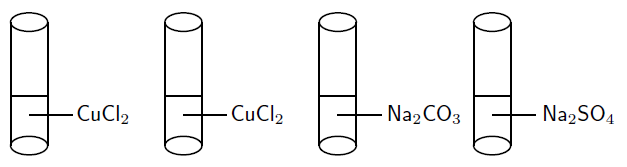
\includegraphics[width=8cm]{col11305.imgs/m38719_CG10C8_004.png} % m38719;CG10C8\_004.png;;;6.0;8.5;
        
      \vspace{2pt}
    \vspace{.1in}
    
    \end{center}

 \end{figure}   

    \addtocounter{footnote}{-0}
    
      \par 
      \label{m38719*id339985}\noindent{}\textbf{Method:}
        \newline
    
      \label{m38719*id339992}\begin{enumerate}[noitemsep, label=\textbf{\arabic*}. ] 
            \label{m38719*uid60}\item Prepare 2 test tubes with approximately 5 ml of dilute Cu(II) chloride solution in each
\label{m38719*uid61}\item Prepare 1 test tube with 5 ml sodium carbonate solution
\label{m38719*uid62}\item Prepare 1 test tube with 5 ml sodium sulphate solution
\label{m38719*uid63}\item Carefully pour the sodium carbonate solution into one of the test tubes containing copper(II) chloride and observe what happens
\label{m38719*uid64}\item Carefully pour the sodium sulphate solution into the second test tube containing copper(II) chloride and observe what happens
\end{enumerate}
        \par 
      \label{m38719*id340060}\noindent{}\textbf{Results:}
        \newline
    
      \label{m38719*id340067}\begin{enumerate}[noitemsep, label=\textbf{\arabic*}. ] 
            \label{m38719*uid65}\item A light blue precipitate forms when sodium carbonate reacts with copper(II) chloride
\label{m38719*uid66}\item No precipitate forms when sodium sulphate reacts with copper(II) chloride
\end{enumerate}
        \par 
      

      \label{m38719*id340106}It is important to understand what happened in the previous demonstration. We will look at what happens in each reaction, step by step.\par 
      \label{m38719*id340110}\begin{enumerate}[noitemsep, label=\textbf{\arabic*}. ] 
            \label{m38719*uid67}\item \textbf{Reaction 1:} Sodium carbonate reacts with copper(II) chloride.\newline
    
When these compounds react, a number of ions are present in solution: \begin{math}{\mathrm{Cu}}^{2+}\end{math}, \begin{math}{\mathrm{Cl}}^{-}\end{math}, \begin{math}{\mathrm{Na}}^{+}\end{math} and \begin{math}\mathrm{CO}_{3}^{2-}\end{math}.
Because there are lots of ions in solution, they will collide with each other and may recombine in different ways. The product that forms may be insoluble, in which case a precipitate will form, or the product will be soluble, in which case the ions will go back into solution. Let's see how the ions in this example could have combined with each other:
\label{m38719*id753}\nopagebreak\noindent{}
\settowidth{\mymathboxwidth}{\begin{equation}
    {\mathrm{Cu}}^{2+}+\mathrm{CO}_{3}^{2-}\to {\mathrm{CuCO}}_{3}\tag{17.14}
      \end{equation}
    }
    \typeout{Columnwidth = \the\columnwidth}\typeout{math as usual width = \the\mymathboxwidth}
    \ifthenelse{\lengthtest{\mymathboxwidth < \columnwidth}}{% if the math fits, do it again, for real
    \begin{equation}
    {\mathrm{Cu}}^{2+}+\mathrm{CO}_{3}^{2-}\to {\mathrm{CuCO}}_{3}\tag{17.14}
      \end{equation}
    }{% else, if it doesn't fit
    \setlength{\mymathboxwidth}{\columnwidth}
      \addtolength{\mymathboxwidth}{-48pt}
    \par\vspace{12pt}\noindent\begin{minipage}{\columnwidth}
    \parbox[t]{\mymathboxwidth}{\large\begin{math}
    {\mathrm{Cu}}^{2+}+\mathrm{CO}_{3}^{2-}\to {\mathrm{CuCO}}_{3}\end{math}}\hfill
    \parbox[t]{48pt}{\raggedleft 
    (17.14)}
    \end{minipage}\vspace{12pt}\par
    }% end of conditional for this bit of math
    \typeout{math as usual width = \the\mymathboxwidth}
    
\label{m38719*id7546}\nopagebreak\noindent{}
\settowidth{\mymathboxwidth}{\begin{equation}
    {\mathrm{Cu}}^{2+}+2{\mathrm{Cl}}^{-}\to {\mathrm{CuCl}}_{2}\tag{17.15}
      \end{equation}
    }
    \typeout{Columnwidth = \the\columnwidth}\typeout{math as usual width = \the\mymathboxwidth}
    \ifthenelse{\lengthtest{\mymathboxwidth < \columnwidth}}{% if the math fits, do it again, for real
    \begin{equation}
    {\mathrm{Cu}}^{2+}+2{\mathrm{Cl}}^{-}\to {\mathrm{CuCl}}_{2}\tag{17.15}
      \end{equation}
    }{% else, if it doesn't fit
    \setlength{\mymathboxwidth}{\columnwidth}
      \addtolength{\mymathboxwidth}{-48pt}
    \par\vspace{12pt}\noindent\begin{minipage}{\columnwidth}
    \parbox[t]{\mymathboxwidth}{\large\begin{math}
    {\mathrm{Cu}}^{2+}+2{\mathrm{Cl}}^{-}\to {\mathrm{CuCl}}_{2}\end{math}}\hfill
    \parbox[t]{48pt}{\raggedleft 
    (17.15)}
    \end{minipage}\vspace{12pt}\par
    }% end of conditional for this bit of math
    \typeout{math as usual width = \the\mymathboxwidth}
    

\label{m38719*id7866}\nopagebreak\noindent{}\settowidth{\mymathboxwidth}{\begin{equation}
    {\mathrm{Na}}^{+}+{\mathrm{Cl}}^{-}\to \mathrm{NaCl}\tag{17.16}
      \end{equation}
    }
    \typeout{Columnwidth = \the\columnwidth}\typeout{math as usual width = \the\mymathboxwidth}
    \ifthenelse{\lengthtest{\mymathboxwidth < \columnwidth}}{% if the math fits, do it again, for real
    \begin{equation}
    {\mathrm{Na}}^{+}+{\mathrm{Cl}}^{-}\to \mathrm{NaCl}\tag{17.16}
      \end{equation}
    }{% else, if it doesn't fit
    \setlength{\mymathboxwidth}{\columnwidth}
      \addtolength{\mymathboxwidth}{-48pt}
    \par\vspace{12pt}\noindent\begin{minipage}{\columnwidth}
    \parbox[t]{\mymathboxwidth}{\large\begin{math}
    {\mathrm{Na}}^{+}+{\mathrm{Cl}}^{-}\to \mathrm{NaCl}\end{math}}\hfill
    \parbox[t]{48pt}{\raggedleft 
    (17.16)}
    \end{minipage}\vspace{12pt}\par
    }% end of conditional for this bit of math
    \typeout{math as usual width = \the\mymathboxwidth}
    
\label{m38719*id76576}\nopagebreak\noindent{}\settowidth{\mymathboxwidth}{\begin{equation}
    2{\mathrm{Na}}^{+}+\mathrm{CO}_{3}^{2-}\to {\mathrm{Na}}_{2}{\mathrm{CO}}_{3}\tag{17.17}
      \end{equation}
    }
    \typeout{Columnwidth = \the\columnwidth}\typeout{math as usual width = \the\mymathboxwidth}
    \ifthenelse{\lengthtest{\mymathboxwidth < \columnwidth}}{% if the math fits, do it again, for real
    \begin{equation}
    2{\mathrm{Na}}^{+}+\mathrm{CO}_{3}^{2-}\to {\mathrm{Na}}_{2}{\mathrm{CO}}_{3}\tag{17.17}
      \end{equation}
    }{% else, if it doesn't fit
    \setlength{\mymathboxwidth}{\columnwidth}
      \addtolength{\mymathboxwidth}{-48pt}
    \par\vspace{12pt}\noindent\begin{minipage}{\columnwidth}
    \parbox[t]{\mymathboxwidth}{\large\begin{math}
    2{\mathrm{Na}}^{+}+\mathrm{CO}_{3}^{2-}\to {\mathrm{Na}}_{2}{\mathrm{CO}}_{3}\end{math}}\hfill
    \parbox[t]{48pt}{\raggedleft 
    (17.17)}
    \end{minipage}\vspace{12pt}\par
    }% end of conditional for this bit of math
    \typeout{math as usual width = \the\mymathboxwidth}
    

You can automatically exclude the reactions where sodium carbonate and copper(II) chloride are the products because these were the initial reactants. You also know that sodium chloride (\begin{math}\mathrm{NaCl}\end{math}) is soluble in water, so the remaining product (copper carbonate) must be the one that is insoluble. It is also possible to look up which salts are soluble and which are insoluble. If you do this, you will find that most carbonates are insoluble, therefore the precipitate that forms in this reaction must be \begin{math}{\mathrm{CuCO}}_{3}\end{math}. The reaction that has taken place between the ions in solution is as follows:
\label{m38719*id7543}\nopagebreak\noindent{}\settowidth{\mymathboxwidth}{\begin{equation}
    2{\mathrm{Na}}^{+}+\mathrm{CO}_{3}^{2-}+{\mathrm{Cu}}^{2+}+2{\mathrm{Cl}}^{-}\to {\mathrm{CuCO}}_{3}+2{\mathrm{Na}}^{+}+2{\mathrm{Cl}}^{-}\tag{17.18}
      \end{equation}
    }
    \typeout{Columnwidth = \the\columnwidth}\typeout{math as usual width = \the\mymathboxwidth}
    \ifthenelse{\lengthtest{\mymathboxwidth < \columnwidth}}{% if the math fits, do it again, for real
    \begin{equation}
    2{\mathrm{Na}}^{+}+\mathrm{CO}_{3}^{2-}+{\mathrm{Cu}}^{2+}+2{\mathrm{Cl}}^{-}\to {\mathrm{CuCO}}_{3}+2{\mathrm{Na}}^{+}+2{\mathrm{Cl}}^{-}\tag{17.18}
      \end{equation}
    }{% else, if it doesn't fit
    \setlength{\mymathboxwidth}{\columnwidth}
      \addtolength{\mymathboxwidth}{-48pt}
    \par\vspace{12pt}\noindent\begin{minipage}{\columnwidth}
    \parbox[t]{\mymathboxwidth}{\large\begin{math}
    2{\mathrm{Na}}^{+}+\mathrm{CO}_{3}^{2-}+{\mathrm{Cu}}^{2+}+2{\mathrm{Cl}}^{-}\to {\mathrm{CuCO}}_{3}+2{\mathrm{Na}}^{+}+2{\mathrm{Cl}}^{-}\end{math}}\hfill
    \parbox[t]{48pt}{\raggedleft 
    (17.18)}
    \end{minipage}\vspace{12pt}\par
    }% end of conditional for this bit of math
    \typeout{math as usual width = \the\mymathboxwidth}
    \label{m38719*uid68}\item \textbf{Reaction 2:} Sodium sulphate reacts with copper(II) chloride.\newline
    
The ions that are present in solution are \begin{math}{\mathrm{Cu}}^{2+}\end{math}, \begin{math}{\mathrm{Cl}}^{-}\end{math}, \begin{math}{\mathrm{Na}}^{+}\end{math} and \begin{math}\mathrm{SO}_{4}^{2-}\end{math}.
The ions collide with each other and may recombine in different ways. The possible combinations of the ions are as follows:
\label{m38719*id763}\nopagebreak\noindent{}
\settowidth{\mymathboxwidth}{\begin{equation}
    {\mathrm{Cu}}^{2+}+\mathrm{SO}_{4}^{2-}\to {\mathrm{CuSO}}_{4}\tag{17.19}
      \end{equation}
    }
    \typeout{Columnwidth = \the\columnwidth}\typeout{math as usual width = \the\mymathboxwidth}
    \ifthenelse{\lengthtest{\mymathboxwidth < \columnwidth}}{% if the math fits, do it again, for real
    \begin{equation}
    {\mathrm{Cu}}^{2+}+\mathrm{SO}_{4}^{2-}\to {\mathrm{CuSO}}_{4}\tag{17.19}
      \end{equation}
    }{% else, if it doesn't fit
    \setlength{\mymathboxwidth}{\columnwidth}
      \addtolength{\mymathboxwidth}{-48pt}
    \par\vspace{12pt}\noindent\begin{minipage}{\columnwidth}
    \parbox[t]{\mymathboxwidth}{\large\begin{math}
    {\mathrm{Cu}}^{2+}+\mathrm{SO}_{4}^{2-}\to {\mathrm{CuSO}}_{4}\end{math}}\hfill
    \parbox[t]{48pt}{\raggedleft 
    (17.19)}
    \end{minipage}\vspace{12pt}\par
    }% end of conditional for this bit of math
    \typeout{math as usual width = \the\mymathboxwidth}
    
\label{m38719*id75876}\nopagebreak\noindent{}
\settowidth{\mymathboxwidth}{\begin{equation}
    {\mathrm{Cu}}^{2+}+2{\mathrm{Cl}}^{-}\to {\mathrm{CuCl}}_{2}\tag{17.20}
      \end{equation}
    }
    \typeout{Columnwidth = \the\columnwidth}\typeout{math as usual width = \the\mymathboxwidth}
    \ifthenelse{\lengthtest{\mymathboxwidth < \columnwidth}}{% if the math fits, do it again, for real
    \begin{equation}
    {\mathrm{Cu}}^{2+}+2{\mathrm{Cl}}^{-}\to {\mathrm{CuCl}}_{2}\tag{17.20}
      \end{equation}
    }{% else, if it doesn't fit
    \setlength{\mymathboxwidth}{\columnwidth}
      \addtolength{\mymathboxwidth}{-48pt}
    \par\vspace{12pt}\noindent\begin{minipage}{\columnwidth}
    \parbox[t]{\mymathboxwidth}{\large\begin{math}
    {\mathrm{Cu}}^{2+}+2{\mathrm{Cl}}^{-}\to {\mathrm{CuCl}}_{2}\end{math}}\hfill
    \parbox[t]{48pt}{\raggedleft 
    (17.20)}
    \end{minipage}\vspace{12pt}\par
    }% end of conditional for this bit of math
    \typeout{math as usual width = \the\mymathboxwidth}
    
\label{m38719*id75745}\nopagebreak\noindent{}
\settowidth{\mymathboxwidth}{\begin{equation}
    {\mathrm{Na}}^{+}+{\mathrm{Cl}}^{-}\to \mathrm{NaCl}\tag{17.21}
      \end{equation}
    }
    \typeout{Columnwidth = \the\columnwidth}\typeout{math as usual width = \the\mymathboxwidth}
    \ifthenelse{\lengthtest{\mymathboxwidth < \columnwidth}}{% if the math fits, do it again, for real
    \begin{equation}
    {\mathrm{Na}}^{+}+{\mathrm{Cl}}^{-}\to \mathrm{NaCl}\tag{17.21}
      \end{equation}
    }{% else, if it doesn't fit
    \setlength{\mymathboxwidth}{\columnwidth}
      \addtolength{\mymathboxwidth}{-48pt}
    \par\vspace{12pt}\noindent\begin{minipage}{\columnwidth}
    \parbox[t]{\mymathboxwidth}{\large\begin{math}
    {\mathrm{Na}}^{+}+{\mathrm{Cl}}^{-}\to \mathrm{NaCl}\end{math}}\hfill
    \parbox[t]{48pt}{\raggedleft 
    (17.21)}
    \end{minipage}\vspace{12pt}\par
    }% end of conditional for this bit of math
    \typeout{math as usual width = \the\mymathboxwidth}
    
\label{m38719*id75775}\nopagebreak\noindent{}
\settowidth{\mymathboxwidth}{\begin{equation}
    {\mathrm{Na}}^{+}+\mathrm{SO}_{4}^{2-}\to {\mathrm{Na}}_{2}{\mathrm{SO}}_{4}\tag{17.22}
      \end{equation}
    }
    \typeout{Columnwidth = \the\columnwidth}\typeout{math as usual width = \the\mymathboxwidth}
    \ifthenelse{\lengthtest{\mymathboxwidth < \columnwidth}}{% if the math fits, do it again, for real
    \begin{equation}
    {\mathrm{Na}}^{+}+\mathrm{SO}_{4}^{2-}\to {\mathrm{Na}}_{2}{\mathrm{SO}}_{4}\tag{17.22}
      \end{equation}
    }{% else, if it doesn't fit
    \setlength{\mymathboxwidth}{\columnwidth}
      \addtolength{\mymathboxwidth}{-48pt}
    \par\vspace{12pt}\noindent\begin{minipage}{\columnwidth}
    \parbox[t]{\mymathboxwidth}{\large\begin{math}
    {\mathrm{Na}}^{+}+\mathrm{SO}_{4}^{2-}\to {\mathrm{Na}}_{2}{\mathrm{SO}}_{4}\end{math}}\hfill
    \parbox[t]{48pt}{\raggedleft 
    (17.22)}
    \end{minipage}\vspace{12pt}\par
    }% end of conditional for this bit of math
    \typeout{math as usual width = \the\mymathboxwidth}
    

If we look up which of these salts are soluble and which are insoluble, we see that most chlorides and most sulphates are soluble. This is why no precipitate forms in this second reaction. Even when the ions recombine, they immediately separate and go back into solution. The reaction that has taken place between the ions in solution is as follows:
\label{m38719*id74443}\nopagebreak\noindent{}\settowidth{\mymathboxwidth}{\begin{equation}
    2{\mathrm{Na}}^{+}+\mathrm{SO}_{4}^{2-}+{\mathrm{Cu}}^{2+}+2{\mathrm{Cl}}^{-}\to 2{\mathrm{Na}}^{+}+\mathrm{SO}_{4}^{2-}+{\mathrm{Cu}}^{2+}+2{\mathrm{Cl}}^{-}\tag{17.23}
      \end{equation}
    }
    \typeout{Columnwidth = \the\columnwidth}\typeout{math as usual width = \the\mymathboxwidth}
    \ifthenelse{\lengthtest{\mymathboxwidth < \columnwidth}}{% if the math fits, do it again, for real
    \begin{equation}
    2{\mathrm{Na}}^{+}+\mathrm{SO}_{4}^{2-}+{\mathrm{Cu}}^{2+}+2{\mathrm{Cl}}^{-}\to 2{\mathrm{Na}}^{+}+\mathrm{SO}_{4}^{2-}+{\mathrm{Cu}}^{2+}+2{\mathrm{Cl}}^{-}\tag{17.23}
      \end{equation}
    }{% else, if it doesn't fit
    \setlength{\mymathboxwidth}{\columnwidth}
      \addtolength{\mymathboxwidth}{-48pt}
    \par\vspace{12pt}\noindent\begin{minipage}{\columnwidth}
    \parbox[t]{\mymathboxwidth}{\large\begin{math}
    2{\mathrm{Na}}^{+}+\mathrm{SO}_{4}^{2-}+{\mathrm{Cu}}^{2+}+2{\mathrm{Cl}}^{-}\to 2{\mathrm{Na}}^{+}+\mathrm{SO}_{4}^{2-}+{\mathrm{Cu}}^{2+}+2{\mathrm{Cl}}^{-}\end{math}}\hfill
    \parbox[t]{48pt}{\raggedleft 
    (17.23)}
    \end{minipage}\vspace{12pt}\par
    }% end of conditional for this bit of math
    \typeout{math as usual width = \the\mymathboxwidth}
    
\end{enumerate}
        
      \label{m38719*id340954}Table 17.2 shows some of the general rules about the solubility of different salts based on a number of investigations:\par 
      
    % \textbf{m38719*uid69}\par
    
    % how many colspecs?  2
          % name: cnx:colspec
            % colnum: 1
            % colwidth: 10*
            % latex-name: columna
            % colname: 
            % align/tgroup-align/default: //left
            % -------------------------
            % name: cnx:colspec
            % colnum: 2
            % colwidth: 10*
            % latex-name: columnb
            % colname: 
            % align/tgroup-align/default: //left
            % -------------------------
      
    
    \setlength\mytablespace{4\tabcolsep}
    \addtolength\mytablespace{3\arrayrulewidth}
    \setlength\mytablewidth{\linewidth}
        
    
    \setlength\mytableroom{\mytablewidth}
    \addtolength\mytableroom{-\mytablespace}
    
    \setlength\myfixedwidth{0pt}
    \setlength\mystarwidth{\mytableroom}
        \addtolength\mystarwidth{-\myfixedwidth}
        \divide\mystarwidth 20
        
    
      % ----- Begin capturing width of table in LR mode woof
      \settowidth{\mytableboxwidth}{\begin{tabular}[t]{|l|l|}\hline
    % count in rowspan-info-nodeset: 2
    % align/colidx: left,1
    
    % rowcount: '0' | start: 'false' | colidx: '1'
    
        % Formatting a regular cell and recurring on the next sibling
        
                \textbf{Salt}
               &
      % align/colidx: left,2
    
    % rowcount: '0' | start: 'false' | colidx: '2'
    
        % Formatting a regular cell and recurring on the next sibling
        
                \textbf{Solubility}
              % make-rowspan-placeholders
    % rowspan info: col1 '0' | 'false' | '' || col2 '0' | 'false' | ''
     \tabularnewline\cline{1-1}\cline{2-2}
      %--------------------------------------------------------------------
    % align/colidx: left,1
    
    % rowcount: '0' | start: 'false' | colidx: '1'
    
        % Formatting a regular cell and recurring on the next sibling
        Nitrates &
      % align/colidx: left,2
    
    % rowcount: '0' | start: 'false' | colidx: '2'
    
        % Formatting a regular cell and recurring on the next sibling
        All are soluble% make-rowspan-placeholders
    % rowspan info: col1 '0' | 'false' | '' || col2 '0' | 'false' | ''
     \tabularnewline\cline{1-1}\cline{2-2}
      %--------------------------------------------------------------------
    % align/colidx: left,1
    
    % rowcount: '0' | start: 'false' | colidx: '1'
    
        % Formatting a regular cell and recurring on the next sibling
        Potassium, sodium and ammonium salts &
      % align/colidx: left,2
    
    % rowcount: '0' | start: 'false' | colidx: '2'
    
        % Formatting a regular cell and recurring on the next sibling
        All are soluble% make-rowspan-placeholders
    % rowspan info: col1 '0' | 'false' | '' || col2 '0' | 'false' | ''
     \tabularnewline\cline{1-1}\cline{2-2}
      %--------------------------------------------------------------------
    % align/colidx: left,1
    
    % rowcount: '0' | start: 'false' | colidx: '1'
    
        % Formatting a regular cell and recurring on the next sibling
        Chlorides, bromides and iodides &
      % align/colidx: left,2
    
    % rowcount: '0' | start: 'false' | colidx: '2'
    
        % Formatting a regular cell and recurring on the next sibling
        All are soluble except silver, lead(II) and mercury(II) salts (e.g. silver chloride)% make-rowspan-placeholders
    % rowspan info: col1 '0' | 'false' | '' || col2 '0' | 'false' | ''
     \tabularnewline\cline{1-1}\cline{2-2}
      %--------------------------------------------------------------------
    % align/colidx: left,1
    
    % rowcount: '0' | start: 'false' | colidx: '1'
    
        % Formatting a regular cell and recurring on the next sibling
        Sulphates &
      % align/colidx: left,2
    
    % rowcount: '0' | start: 'false' | colidx: '2'
    
        % Formatting a regular cell and recurring on the next sibling
        All are soluble except lead(II) sulphate, barium sulphate and calcium sulphate% make-rowspan-placeholders
    % rowspan info: col1 '0' | 'false' | '' || col2 '0' | 'false' | ''
     \tabularnewline\cline{1-1}\cline{2-2}
      %--------------------------------------------------------------------
    % align/colidx: left,1
    
    % rowcount: '0' | start: 'false' | colidx: '1'
    
        % Formatting a regular cell and recurring on the next sibling
        Carbonates &
      % align/colidx: left,2
    
    % rowcount: '0' | start: 'false' | colidx: '2'
    
        % Formatting a regular cell and recurring on the next sibling
        All are insoluble except those of potassium, sodium and ammonium% make-rowspan-placeholders
    % rowspan info: col1 '0' | 'false' | '' || col2 '0' | 'false' | ''
     \tabularnewline\cline{1-1}\cline{2-2}
      %--------------------------------------------------------------------
    % align/colidx: left,1
    
    % rowcount: '0' | start: 'false' | colidx: '1'
    
        % Formatting a regular cell and recurring on the next sibling
        Compounds with fluorine &
      % align/colidx: left,2
    
    % rowcount: '0' | start: 'false' | colidx: '2'
    
        % Formatting a regular cell and recurring on the next sibling
        Almost all are soluble except those of magnesium, calcium, strontium (II), barium (II) and lead (II)% make-rowspan-placeholders
    % rowspan info: col1 '0' | 'false' | '' || col2 '0' | 'false' | ''
     \tabularnewline\cline{1-1}\cline{2-2}
      %--------------------------------------------------------------------
    % align/colidx: left,1
    
    % rowcount: '0' | start: 'false' | colidx: '1'
    
        % Formatting a regular cell and recurring on the next sibling
        Perchlorates and acetates &
      % align/colidx: left,2
    
    % rowcount: '0' | start: 'false' | colidx: '2'
    
        % Formatting a regular cell and recurring on the next sibling
        All are soluble% make-rowspan-placeholders
    % rowspan info: col1 '0' | 'false' | '' || col2 '0' | 'false' | ''
     \tabularnewline\cline{1-1}\cline{2-2}
      %--------------------------------------------------------------------
    % align/colidx: left,1
    
    % rowcount: '0' | start: 'false' | colidx: '1'
    
        % Formatting a regular cell and recurring on the next sibling
        Chlorates &
      % align/colidx: left,2
    
    % rowcount: '0' | start: 'false' | colidx: '2'
    
        % Formatting a regular cell and recurring on the next sibling
        All are soluble except potassium chlorate% make-rowspan-placeholders
    % rowspan info: col1 '0' | 'false' | '' || col2 '0' | 'false' | ''
     \tabularnewline\cline{1-1}\cline{2-2}
      %--------------------------------------------------------------------
    % align/colidx: left,1
    
    % rowcount: '0' | start: 'false' | colidx: '1'
    
        % Formatting a regular cell and recurring on the next sibling
        Metal hydroxides and oxides &
      % align/colidx: left,2
    
    % rowcount: '0' | start: 'false' | colidx: '2'
    
        % Formatting a regular cell and recurring on the next sibling
        Most are insoluble% make-rowspan-placeholders
    % rowspan info: col1 '0' | 'false' | '' || col2 '0' | 'false' | ''
     \tabularnewline\cline{1-1}\cline{2-2}
      %--------------------------------------------------------------------
    \end{tabular}} % end mytableboxwidth set
      \addtocounter{footnote}{-0}
      
      % ----- End capturing width of table in LR mode
    
        % ----- LR or paragraph mode: must test
        % ----- Begin capturing height of table
        \settoheight{\mytableboxheight}{\begin{tabular}[t]{|l|l|}\hline
    % count in rowspan-info-nodeset: 2
    % align/colidx: left,1
    
    % rowcount: '0' | start: 'false' | colidx: '1'
    
        % Formatting a regular cell and recurring on the next sibling
        
                \textbf{Salt}
               &
      % align/colidx: left,2
    
    % rowcount: '0' | start: 'false' | colidx: '2'
    
        % Formatting a regular cell and recurring on the next sibling
        
                \textbf{Solubility}
              % make-rowspan-placeholders
    % rowspan info: col1 '0' | 'false' | '' || col2 '0' | 'false' | ''
     \tabularnewline\cline{1-1}\cline{2-2}
      %--------------------------------------------------------------------
    % align/colidx: left,1
    
    % rowcount: '0' | start: 'false' | colidx: '1'
    
        % Formatting a regular cell and recurring on the next sibling
        Nitrates &
      % align/colidx: left,2
    
    % rowcount: '0' | start: 'false' | colidx: '2'
    
        % Formatting a regular cell and recurring on the next sibling
        All are soluble% make-rowspan-placeholders
    % rowspan info: col1 '0' | 'false' | '' || col2 '0' | 'false' | ''
     \tabularnewline\cline{1-1}\cline{2-2}
      %--------------------------------------------------------------------
    % align/colidx: left,1
    
    % rowcount: '0' | start: 'false' | colidx: '1'
    
        % Formatting a regular cell and recurring on the next sibling
        Potassium, sodium and ammonium salts &
      % align/colidx: left,2
    
    % rowcount: '0' | start: 'false' | colidx: '2'
    
        % Formatting a regular cell and recurring on the next sibling
        All are soluble% make-rowspan-placeholders
    % rowspan info: col1 '0' | 'false' | '' || col2 '0' | 'false' | ''
     \tabularnewline\cline{1-1}\cline{2-2}
      %--------------------------------------------------------------------
    % align/colidx: left,1
    
    % rowcount: '0' | start: 'false' | colidx: '1'
    
        % Formatting a regular cell and recurring on the next sibling
        Chlorides, bromides and iodides &
      % align/colidx: left,2
    
    % rowcount: '0' | start: 'false' | colidx: '2'
    
        % Formatting a regular cell and recurring on the next sibling
        All are soluble except silver, lead(II) and mercury(II) salts (e.g. silver chloride)% make-rowspan-placeholders
    % rowspan info: col1 '0' | 'false' | '' || col2 '0' | 'false' | ''
     \tabularnewline\cline{1-1}\cline{2-2}
      %--------------------------------------------------------------------
    % align/colidx: left,1
    
    % rowcount: '0' | start: 'false' | colidx: '1'
    
        % Formatting a regular cell and recurring on the next sibling
        Sulphates &
      % align/colidx: left,2
    
    % rowcount: '0' | start: 'false' | colidx: '2'
    
        % Formatting a regular cell and recurring on the next sibling
        All are soluble except lead(II) sulphate, barium sulphate and calcium sulphate% make-rowspan-placeholders
    % rowspan info: col1 '0' | 'false' | '' || col2 '0' | 'false' | ''
     \tabularnewline\cline{1-1}\cline{2-2}
      %--------------------------------------------------------------------
    % align/colidx: left,1
    
    % rowcount: '0' | start: 'false' | colidx: '1'
    
        % Formatting a regular cell and recurring on the next sibling
        Carbonates &
      % align/colidx: left,2
    
    % rowcount: '0' | start: 'false' | colidx: '2'
    
        % Formatting a regular cell and recurring on the next sibling
        All are insoluble except those of potassium, sodium and ammonium% make-rowspan-placeholders
    % rowspan info: col1 '0' | 'false' | '' || col2 '0' | 'false' | ''
     \tabularnewline\cline{1-1}\cline{2-2}
      %--------------------------------------------------------------------
    % align/colidx: left,1
    
    % rowcount: '0' | start: 'false' | colidx: '1'
    
        % Formatting a regular cell and recurring on the next sibling
        Compounds with fluorine &
      % align/colidx: left,2
    
    % rowcount: '0' | start: 'false' | colidx: '2'
    
        % Formatting a regular cell and recurring on the next sibling
        Almost all are soluble except those of magnesium, calcium, strontium (II), barium (II) and lead (II)% make-rowspan-placeholders
    % rowspan info: col1 '0' | 'false' | '' || col2 '0' | 'false' | ''
     \tabularnewline\cline{1-1}\cline{2-2}
      %--------------------------------------------------------------------
    % align/colidx: left,1
    
    % rowcount: '0' | start: 'false' | colidx: '1'
    
        % Formatting a regular cell and recurring on the next sibling
        Perchlorates and acetates &
      % align/colidx: left,2
    
    % rowcount: '0' | start: 'false' | colidx: '2'
    
        % Formatting a regular cell and recurring on the next sibling
        All are soluble% make-rowspan-placeholders
    % rowspan info: col1 '0' | 'false' | '' || col2 '0' | 'false' | ''
     \tabularnewline\cline{1-1}\cline{2-2}
      %--------------------------------------------------------------------
    % align/colidx: left,1
    
    % rowcount: '0' | start: 'false' | colidx: '1'
    
        % Formatting a regular cell and recurring on the next sibling
        Chlorates &
      % align/colidx: left,2
    
    % rowcount: '0' | start: 'false' | colidx: '2'
    
        % Formatting a regular cell and recurring on the next sibling
        All are soluble except potassium chlorate% make-rowspan-placeholders
    % rowspan info: col1 '0' | 'false' | '' || col2 '0' | 'false' | ''
     \tabularnewline\cline{1-1}\cline{2-2}
      %--------------------------------------------------------------------
    % align/colidx: left,1
    
    % rowcount: '0' | start: 'false' | colidx: '1'
    
        % Formatting a regular cell and recurring on the next sibling
        Metal hydroxides and oxides &
      % align/colidx: left,2
    
    % rowcount: '0' | start: 'false' | colidx: '2'
    
        % Formatting a regular cell and recurring on the next sibling
        Most are insoluble% make-rowspan-placeholders
    % rowspan info: col1 '0' | 'false' | '' || col2 '0' | 'false' | ''
     \tabularnewline\cline{1-1}\cline{2-2}
      %--------------------------------------------------------------------
    \end{tabular}} % end mytableboxheight set
        \settodepth{\mytableboxdepth}{\begin{tabular}[t]{|l|l|}\hline
    % count in rowspan-info-nodeset: 2
    % align/colidx: left,1
    
    % rowcount: '0' | start: 'false' | colidx: '1'
    
        % Formatting a regular cell and recurring on the next sibling
        
                \textbf{Salt}
               &
      % align/colidx: left,2
    
    % rowcount: '0' | start: 'false' | colidx: '2'
    
        % Formatting a regular cell and recurring on the next sibling
        
                \textbf{Solubility}
              % make-rowspan-placeholders
    % rowspan info: col1 '0' | 'false' | '' || col2 '0' | 'false' | ''
     \tabularnewline\cline{1-1}\cline{2-2}
      %--------------------------------------------------------------------
    % align/colidx: left,1
    
    % rowcount: '0' | start: 'false' | colidx: '1'
    
        % Formatting a regular cell and recurring on the next sibling
        Nitrates &
      % align/colidx: left,2
    
    % rowcount: '0' | start: 'false' | colidx: '2'
    
        % Formatting a regular cell and recurring on the next sibling
        All are soluble% make-rowspan-placeholders
    % rowspan info: col1 '0' | 'false' | '' || col2 '0' | 'false' | ''
     \tabularnewline\cline{1-1}\cline{2-2}
      %--------------------------------------------------------------------
    % align/colidx: left,1
    
    % rowcount: '0' | start: 'false' | colidx: '1'
    
        % Formatting a regular cell and recurring on the next sibling
        Potassium, sodium and ammonium salts &
      % align/colidx: left,2
    
    % rowcount: '0' | start: 'false' | colidx: '2'
    
        % Formatting a regular cell and recurring on the next sibling
        All are soluble% make-rowspan-placeholders
    % rowspan info: col1 '0' | 'false' | '' || col2 '0' | 'false' | ''
     \tabularnewline\cline{1-1}\cline{2-2}
      %--------------------------------------------------------------------
    % align/colidx: left,1
    
    % rowcount: '0' | start: 'false' | colidx: '1'
    
        % Formatting a regular cell and recurring on the next sibling
        Chlorides, bromides and iodides &
      % align/colidx: left,2
    
    % rowcount: '0' | start: 'false' | colidx: '2'
    
        % Formatting a regular cell and recurring on the next sibling
        All are soluble except silver, lead(II) and mercury(II) salts (e.g. silver chloride)% make-rowspan-placeholders
    % rowspan info: col1 '0' | 'false' | '' || col2 '0' | 'false' | ''
     \tabularnewline\cline{1-1}\cline{2-2}
      %--------------------------------------------------------------------
    % align/colidx: left,1
    
    % rowcount: '0' | start: 'false' | colidx: '1'
    
        % Formatting a regular cell and recurring on the next sibling
        Sulphates &
      % align/colidx: left,2
    
    % rowcount: '0' | start: 'false' | colidx: '2'
    
        % Formatting a regular cell and recurring on the next sibling
        All are soluble except lead(II) sulphate, barium sulphate and calcium sulphate% make-rowspan-placeholders
    % rowspan info: col1 '0' | 'false' | '' || col2 '0' | 'false' | ''
     \tabularnewline\cline{1-1}\cline{2-2}
      %--------------------------------------------------------------------
    % align/colidx: left,1
    
    % rowcount: '0' | start: 'false' | colidx: '1'
    
        % Formatting a regular cell and recurring on the next sibling
        Carbonates &
      % align/colidx: left,2
    
    % rowcount: '0' | start: 'false' | colidx: '2'
    
        % Formatting a regular cell and recurring on the next sibling
        All are insoluble except those of potassium, sodium and ammonium% make-rowspan-placeholders
    % rowspan info: col1 '0' | 'false' | '' || col2 '0' | 'false' | ''
     \tabularnewline\cline{1-1}\cline{2-2}
      %--------------------------------------------------------------------
    % align/colidx: left,1
    
    % rowcount: '0' | start: 'false' | colidx: '1'
    
        % Formatting a regular cell and recurring on the next sibling
        Compounds with fluorine &
      % align/colidx: left,2
    
    % rowcount: '0' | start: 'false' | colidx: '2'
    
        % Formatting a regular cell and recurring on the next sibling
        Almost all are soluble except those of magnesium, calcium, strontium (II), barium (II) and lead (II)% make-rowspan-placeholders
    % rowspan info: col1 '0' | 'false' | '' || col2 '0' | 'false' | ''
     \tabularnewline\cline{1-1}\cline{2-2}
      %--------------------------------------------------------------------
    % align/colidx: left,1
    
    % rowcount: '0' | start: 'false' | colidx: '1'
    
        % Formatting a regular cell and recurring on the next sibling
        Perchlorates and acetates &
      % align/colidx: left,2
    
    % rowcount: '0' | start: 'false' | colidx: '2'
    
        % Formatting a regular cell and recurring on the next sibling
        All are soluble% make-rowspan-placeholders
    % rowspan info: col1 '0' | 'false' | '' || col2 '0' | 'false' | ''
     \tabularnewline\cline{1-1}\cline{2-2}
      %--------------------------------------------------------------------
    % align/colidx: left,1
    
    % rowcount: '0' | start: 'false' | colidx: '1'
    
        % Formatting a regular cell and recurring on the next sibling
        Chlorates &
      % align/colidx: left,2
    
    % rowcount: '0' | start: 'false' | colidx: '2'
    
        % Formatting a regular cell and recurring on the next sibling
        All are soluble except potassium chlorate% make-rowspan-placeholders
    % rowspan info: col1 '0' | 'false' | '' || col2 '0' | 'false' | ''
     \tabularnewline\cline{1-1}\cline{2-2}
      %--------------------------------------------------------------------
    % align/colidx: left,1
    
    % rowcount: '0' | start: 'false' | colidx: '1'
    
        % Formatting a regular cell and recurring on the next sibling
        Metal hydroxides and oxides &
      % align/colidx: left,2
    
    % rowcount: '0' | start: 'false' | colidx: '2'
    
        % Formatting a regular cell and recurring on the next sibling
        Most are insoluble% make-rowspan-placeholders
    % rowspan info: col1 '0' | 'false' | '' || col2 '0' | 'false' | ''
     \tabularnewline\cline{1-1}\cline{2-2}
      %--------------------------------------------------------------------
    \end{tabular}} % end mytableboxdepth set
        \addtolength{\mytableboxheight}{\mytableboxdepth}
        % ----- End capturing height of table
        \addtocounter{footnote}{-0}
        
        \ifthenelse{\mytableboxwidth<\textwidth}{% the table fits in LR mode
          \addtolength{\mytableboxwidth}{-\mytablespace}
          \typeout{textheight: \the\textheight}
          \typeout{mytableboxheight: \the\mytableboxheight}
          \typeout{textwidth: \the\textwidth}
          \typeout{mytableboxwidth: \the\mytableboxwidth}
          \ifthenelse{\mytableboxheight<\textheight}{%
        
    % \begin{table}[H]
    % \\ '' '0'
    
        \begin{center}
      
      \label{m38719*uid69}
      
    \noindent
    \begin{tabular}[t]{|l|l|}\hline
    % count in rowspan-info-nodeset: 2
    % align/colidx: left,1
    
    % rowcount: '0' | start: 'false' | colidx: '1'
    
        % Formatting a regular cell and recurring on the next sibling
        
                \textbf{Salt}
               &
      % align/colidx: left,2
    
    % rowcount: '0' | start: 'false' | colidx: '2'
    
        % Formatting a regular cell and recurring on the next sibling
        
                \textbf{Solubility}
              % make-rowspan-placeholders
    % rowspan info: col1 '0' | 'false' | '' || col2 '0' | 'false' | ''
     \tabularnewline\cline{1-1}\cline{2-2}
      %--------------------------------------------------------------------
    % align/colidx: left,1
    
    % rowcount: '0' | start: 'false' | colidx: '1'
    
        % Formatting a regular cell and recurring on the next sibling
        Nitrates &
      % align/colidx: left,2
    
    % rowcount: '0' | start: 'false' | colidx: '2'
    
        % Formatting a regular cell and recurring on the next sibling
        All are soluble% make-rowspan-placeholders
    % rowspan info: col1 '0' | 'false' | '' || col2 '0' | 'false' | ''
     \tabularnewline\cline{1-1}\cline{2-2}
      %--------------------------------------------------------------------
    % align/colidx: left,1
    
    % rowcount: '0' | start: 'false' | colidx: '1'
    
        % Formatting a regular cell and recurring on the next sibling
        Potassium, sodium and ammonium salts &
      % align/colidx: left,2
    
    % rowcount: '0' | start: 'false' | colidx: '2'
    
        % Formatting a regular cell and recurring on the next sibling
        All are soluble% make-rowspan-placeholders
    % rowspan info: col1 '0' | 'false' | '' || col2 '0' | 'false' | ''
     \tabularnewline\cline{1-1}\cline{2-2}
      %--------------------------------------------------------------------
    % align/colidx: left,1
    
    % rowcount: '0' | start: 'false' | colidx: '1'
    
        % Formatting a regular cell and recurring on the next sibling
        Chlorides, bromides and iodides &
      % align/colidx: left,2
    
    % rowcount: '0' | start: 'false' | colidx: '2'
    
        % Formatting a regular cell and recurring on the next sibling
        All are soluble except silver, lead(II) and mercury(II) salts (e.g. silver chloride)% make-rowspan-placeholders
    % rowspan info: col1 '0' | 'false' | '' || col2 '0' | 'false' | ''
     \tabularnewline\cline{1-1}\cline{2-2}
      %--------------------------------------------------------------------
    % align/colidx: left,1
    
    % rowcount: '0' | start: 'false' | colidx: '1'
    
        % Formatting a regular cell and recurring on the next sibling
        Sulphates &
      % align/colidx: left,2
    
    % rowcount: '0' | start: 'false' | colidx: '2'
    
        % Formatting a regular cell and recurring on the next sibling
        All are soluble except lead(II) sulphate, barium sulphate and calcium sulphate% make-rowspan-placeholders
    % rowspan info: col1 '0' | 'false' | '' || col2 '0' | 'false' | ''
     \tabularnewline\cline{1-1}\cline{2-2}
      %--------------------------------------------------------------------
    % align/colidx: left,1
    
    % rowcount: '0' | start: 'false' | colidx: '1'
    
        % Formatting a regular cell and recurring on the next sibling
        Carbonates &
      % align/colidx: left,2
    
    % rowcount: '0' | start: 'false' | colidx: '2'
    
        % Formatting a regular cell and recurring on the next sibling
        All are insoluble except those of potassium, sodium and ammonium% make-rowspan-placeholders
    % rowspan info: col1 '0' | 'false' | '' || col2 '0' | 'false' | ''
     \tabularnewline\cline{1-1}\cline{2-2}
      %--------------------------------------------------------------------
    % align/colidx: left,1
    
    % rowcount: '0' | start: 'false' | colidx: '1'
    
        % Formatting a regular cell and recurring on the next sibling
        Compounds with fluorine &
      % align/colidx: left,2
    
    % rowcount: '0' | start: 'false' | colidx: '2'
    
        % Formatting a regular cell and recurring on the next sibling
        Almost all are soluble except those of magnesium, calcium, strontium (II), barium (II) and lead (II)% make-rowspan-placeholders
    % rowspan info: col1 '0' | 'false' | '' || col2 '0' | 'false' | ''
     \tabularnewline\cline{1-1}\cline{2-2}
      %--------------------------------------------------------------------
    % align/colidx: left,1
    
    % rowcount: '0' | start: 'false' | colidx: '1'
    
        % Formatting a regular cell and recurring on the next sibling
        Perchlorates and acetates &
      % align/colidx: left,2
    
    % rowcount: '0' | start: 'false' | colidx: '2'
    
        % Formatting a regular cell and recurring on the next sibling
        All are soluble% make-rowspan-placeholders
    % rowspan info: col1 '0' | 'false' | '' || col2 '0' | 'false' | ''
     \tabularnewline\cline{1-1}\cline{2-2}
      %--------------------------------------------------------------------
    % align/colidx: left,1
    
    % rowcount: '0' | start: 'false' | colidx: '1'
    
        % Formatting a regular cell and recurring on the next sibling
        Chlorates &
      % align/colidx: left,2
    
    % rowcount: '0' | start: 'false' | colidx: '2'
    
        % Formatting a regular cell and recurring on the next sibling
        All are soluble except potassium chlorate% make-rowspan-placeholders
    % rowspan info: col1 '0' | 'false' | '' || col2 '0' | 'false' | ''
     \tabularnewline\cline{1-1}\cline{2-2}
      %--------------------------------------------------------------------
    % align/colidx: left,1
    
    % rowcount: '0' | start: 'false' | colidx: '1'
    
        % Formatting a regular cell and recurring on the next sibling
        Metal hydroxides and oxides &
      % align/colidx: left,2
    
    % rowcount: '0' | start: 'false' | colidx: '2'
    
        % Formatting a regular cell and recurring on the next sibling
        Most are insoluble% make-rowspan-placeholders
    % rowspan info: col1 '0' | 'false' | '' || col2 '0' | 'false' | ''
     \tabularnewline\cline{1-1}\cline{2-2}
      %--------------------------------------------------------------------
    \end{tabular}
      \end{center}
    \begin{center}{\small\bfseries Table 17.2}: General rules for the solubility of salts\end{center}
    %\end{table}
    
    \addtocounter{footnote}{-0}
    
          }{ % else
        
    % \begin{table}[H]
    % \\ '' '0'
    
        \begin{center}
      
      \label{m38719*uid69}
      
    \noindent
    \tabletail{%
        \hline
        \multicolumn{2}{|p{\mytableboxwidth}|}{\raggedleft \small \sl continued on next page}\\
        \hline
      }
      \tablelasttail{}
      \begin{xtabular}[t]{|l|l|}\hline
    % count in rowspan-info-nodeset: 2
    % align/colidx: left,1
    
    % rowcount: '0' | start: 'false' | colidx: '1'
    
        % Formatting a regular cell and recurring on the next sibling
        
                \textbf{Salt}
               &
      % align/colidx: left,2
    
    % rowcount: '0' | start: 'false' | colidx: '2'
    
        % Formatting a regular cell and recurring on the next sibling
        
                \textbf{Solubility}
              % make-rowspan-placeholders
    % rowspan info: col1 '0' | 'false' | '' || col2 '0' | 'false' | ''
     \tabularnewline\cline{1-1}\cline{2-2}
      %--------------------------------------------------------------------
    % align/colidx: left,1
    
    % rowcount: '0' | start: 'false' | colidx: '1'
    
        % Formatting a regular cell and recurring on the next sibling
        Nitrates &
      % align/colidx: left,2
    
    % rowcount: '0' | start: 'false' | colidx: '2'
    
        % Formatting a regular cell and recurring on the next sibling
        All are soluble% make-rowspan-placeholders
    % rowspan info: col1 '0' | 'false' | '' || col2 '0' | 'false' | ''
     \tabularnewline\cline{1-1}\cline{2-2}
      %--------------------------------------------------------------------
    % align/colidx: left,1
    
    % rowcount: '0' | start: 'false' | colidx: '1'
    
        % Formatting a regular cell and recurring on the next sibling
        Potassium, sodium and ammonium salts &
      % align/colidx: left,2
    
    % rowcount: '0' | start: 'false' | colidx: '2'
    
        % Formatting a regular cell and recurring on the next sibling
        All are soluble% make-rowspan-placeholders
    % rowspan info: col1 '0' | 'false' | '' || col2 '0' | 'false' | ''
     \tabularnewline\cline{1-1}\cline{2-2}
      %--------------------------------------------------------------------
    % align/colidx: left,1
    
    % rowcount: '0' | start: 'false' | colidx: '1'
    
        % Formatting a regular cell and recurring on the next sibling
        Chlorides, bromides and iodides &
      % align/colidx: left,2
    
    % rowcount: '0' | start: 'false' | colidx: '2'
    
        % Formatting a regular cell and recurring on the next sibling
        All are soluble except silver, lead(II) and mercury(II) salts (e.g. silver chloride)% make-rowspan-placeholders
    % rowspan info: col1 '0' | 'false' | '' || col2 '0' | 'false' | ''
     \tabularnewline\cline{1-1}\cline{2-2}
      %--------------------------------------------------------------------
    % align/colidx: left,1
    
    % rowcount: '0' | start: 'false' | colidx: '1'
    
        % Formatting a regular cell and recurring on the next sibling
        Sulphates &
      % align/colidx: left,2
    
    % rowcount: '0' | start: 'false' | colidx: '2'
    
        % Formatting a regular cell and recurring on the next sibling
        All are soluble except lead(II) sulphate, barium sulphate and calcium sulphate% make-rowspan-placeholders
    % rowspan info: col1 '0' | 'false' | '' || col2 '0' | 'false' | ''
     \tabularnewline\cline{1-1}\cline{2-2}
      %--------------------------------------------------------------------
    % align/colidx: left,1
    
    % rowcount: '0' | start: 'false' | colidx: '1'
    
        % Formatting a regular cell and recurring on the next sibling
        Carbonates &
      % align/colidx: left,2
    
    % rowcount: '0' | start: 'false' | colidx: '2'
    
        % Formatting a regular cell and recurring on the next sibling
        All are insoluble except those of potassium, sodium and ammonium% make-rowspan-placeholders
    % rowspan info: col1 '0' | 'false' | '' || col2 '0' | 'false' | ''
     \tabularnewline\cline{1-1}\cline{2-2}
      %--------------------------------------------------------------------
    % align/colidx: left,1
    
    % rowcount: '0' | start: 'false' | colidx: '1'
    
        % Formatting a regular cell and recurring on the next sibling
        Compounds with fluorine &
      % align/colidx: left,2
    
    % rowcount: '0' | start: 'false' | colidx: '2'
    
        % Formatting a regular cell and recurring on the next sibling
        Almost all are soluble except those of magnesium, calcium, strontium (II), barium (II) and lead (II)% make-rowspan-placeholders
    % rowspan info: col1 '0' | 'false' | '' || col2 '0' | 'false' | ''
     \tabularnewline\cline{1-1}\cline{2-2}
      %--------------------------------------------------------------------
    % align/colidx: left,1
    
    % rowcount: '0' | start: 'false' | colidx: '1'
    
        % Formatting a regular cell and recurring on the next sibling
        Perchlorates and acetates &
      % align/colidx: left,2
    
    % rowcount: '0' | start: 'false' | colidx: '2'
    
        % Formatting a regular cell and recurring on the next sibling
        All are soluble% make-rowspan-placeholders
    % rowspan info: col1 '0' | 'false' | '' || col2 '0' | 'false' | ''
     \tabularnewline\cline{1-1}\cline{2-2}
      %--------------------------------------------------------------------
    % align/colidx: left,1
    
    % rowcount: '0' | start: 'false' | colidx: '1'
    
        % Formatting a regular cell and recurring on the next sibling
        Chlorates &
      % align/colidx: left,2
    
    % rowcount: '0' | start: 'false' | colidx: '2'
    
        % Formatting a regular cell and recurring on the next sibling
        All are soluble except potassium chlorate% make-rowspan-placeholders
    % rowspan info: col1 '0' | 'false' | '' || col2 '0' | 'false' | ''
     \tabularnewline\cline{1-1}\cline{2-2}
      %--------------------------------------------------------------------
    % align/colidx: left,1
    
    % rowcount: '0' | start: 'false' | colidx: '1'
    
        % Formatting a regular cell and recurring on the next sibling
        Metal hydroxides and oxides &
      % align/colidx: left,2
    
    % rowcount: '0' | start: 'false' | colidx: '2'
    
        % Formatting a regular cell and recurring on the next sibling
        Most are insoluble% make-rowspan-placeholders
    % rowspan info: col1 '0' | 'false' | '' || col2 '0' | 'false' | ''
     \tabularnewline\cline{1-1}\cline{2-2}
      %--------------------------------------------------------------------
    \end{xtabular}
      \end{center}
    \begin{center}{\small\bfseries Table 17.2}: General rules for the solubility of salts\end{center}
    %\end{table}
    
    \addtocounter{footnote}{-0}
    
          } % 
        }{% else
        % typeset the table in paragraph mode
        % ----- Begin capturing height of table
        \settoheight{\mytableboxheight}{\begin{tabular*}{\mytablewidth}[t]{|p{10\mystarwidth}|p{10\mystarwidth}|}\hline
    % count in rowspan-info-nodeset: 2
    % align/colidx: left,1
    
    % rowcount: '0' | start: 'false' | colidx: '1'
    
        % Formatting a regular cell and recurring on the next sibling
        
                \textbf{Salt}
               &
      % align/colidx: left,2
    
    % rowcount: '0' | start: 'false' | colidx: '2'
    
        % Formatting a regular cell and recurring on the next sibling
        
                \textbf{Solubility}
              % make-rowspan-placeholders
    % rowspan info: col1 '0' | 'false' | '' || col2 '0' | 'false' | ''
     \tabularnewline\cline{1-1}\cline{2-2}
      %--------------------------------------------------------------------
    % align/colidx: left,1
    
    % rowcount: '0' | start: 'false' | colidx: '1'
    
        % Formatting a regular cell and recurring on the next sibling
        Nitrates &
      % align/colidx: left,2
    
    % rowcount: '0' | start: 'false' | colidx: '2'
    
        % Formatting a regular cell and recurring on the next sibling
        All are soluble% make-rowspan-placeholders
    % rowspan info: col1 '0' | 'false' | '' || col2 '0' | 'false' | ''
     \tabularnewline\cline{1-1}\cline{2-2}
      %--------------------------------------------------------------------
    % align/colidx: left,1
    
    % rowcount: '0' | start: 'false' | colidx: '1'
    
        % Formatting a regular cell and recurring on the next sibling
        Potassium, sodium and ammonium salts &
      % align/colidx: left,2
    
    % rowcount: '0' | start: 'false' | colidx: '2'
    
        % Formatting a regular cell and recurring on the next sibling
        All are soluble% make-rowspan-placeholders
    % rowspan info: col1 '0' | 'false' | '' || col2 '0' | 'false' | ''
     \tabularnewline\cline{1-1}\cline{2-2}
      %--------------------------------------------------------------------
    % align/colidx: left,1
    
    % rowcount: '0' | start: 'false' | colidx: '1'
    
        % Formatting a regular cell and recurring on the next sibling
        Chlorides, bromides and iodides &
      % align/colidx: left,2
    
    % rowcount: '0' | start: 'false' | colidx: '2'
    
        % Formatting a regular cell and recurring on the next sibling
        All are soluble except silver, lead(II) and mercury(II) salts (e.g. silver chloride)% make-rowspan-placeholders
    % rowspan info: col1 '0' | 'false' | '' || col2 '0' | 'false' | ''
     \tabularnewline\cline{1-1}\cline{2-2}
      %--------------------------------------------------------------------
    % align/colidx: left,1
    
    % rowcount: '0' | start: 'false' | colidx: '1'
    
        % Formatting a regular cell and recurring on the next sibling
        Sulphates &
      % align/colidx: left,2
    
    % rowcount: '0' | start: 'false' | colidx: '2'
    
        % Formatting a regular cell and recurring on the next sibling
        All are soluble except lead(II) sulphate, barium sulphate and calcium sulphate% make-rowspan-placeholders
    % rowspan info: col1 '0' | 'false' | '' || col2 '0' | 'false' | ''
     \tabularnewline\cline{1-1}\cline{2-2}
      %--------------------------------------------------------------------
    % align/colidx: left,1
    
    % rowcount: '0' | start: 'false' | colidx: '1'
    
        % Formatting a regular cell and recurring on the next sibling
        Carbonates &
      % align/colidx: left,2
    
    % rowcount: '0' | start: 'false' | colidx: '2'
    
        % Formatting a regular cell and recurring on the next sibling
        All are insoluble except those of potassium, sodium and ammonium% make-rowspan-placeholders
    % rowspan info: col1 '0' | 'false' | '' || col2 '0' | 'false' | ''
     \tabularnewline\cline{1-1}\cline{2-2}
      %--------------------------------------------------------------------
    % align/colidx: left,1
    
    % rowcount: '0' | start: 'false' | colidx: '1'
    
        % Formatting a regular cell and recurring on the next sibling
        Compounds with fluorine &
      % align/colidx: left,2
    
    % rowcount: '0' | start: 'false' | colidx: '2'
    
        % Formatting a regular cell and recurring on the next sibling
        Almost all are soluble except those of magnesium, calcium, strontium (II), barium (II) and lead (II)% make-rowspan-placeholders
    % rowspan info: col1 '0' | 'false' | '' || col2 '0' | 'false' | ''
     \tabularnewline\cline{1-1}\cline{2-2}
      %--------------------------------------------------------------------
    % align/colidx: left,1
    
    % rowcount: '0' | start: 'false' | colidx: '1'
    
        % Formatting a regular cell and recurring on the next sibling
        Perchlorates and acetates &
      % align/colidx: left,2
    
    % rowcount: '0' | start: 'false' | colidx: '2'
    
        % Formatting a regular cell and recurring on the next sibling
        All are soluble% make-rowspan-placeholders
    % rowspan info: col1 '0' | 'false' | '' || col2 '0' | 'false' | ''
     \tabularnewline\cline{1-1}\cline{2-2}
      %--------------------------------------------------------------------
    % align/colidx: left,1
    
    % rowcount: '0' | start: 'false' | colidx: '1'
    
        % Formatting a regular cell and recurring on the next sibling
        Chlorates &
      % align/colidx: left,2
    
    % rowcount: '0' | start: 'false' | colidx: '2'
    
        % Formatting a regular cell and recurring on the next sibling
        All are soluble except potassium chlorate% make-rowspan-placeholders
    % rowspan info: col1 '0' | 'false' | '' || col2 '0' | 'false' | ''
     \tabularnewline\cline{1-1}\cline{2-2}
      %--------------------------------------------------------------------
    % align/colidx: left,1
    
    % rowcount: '0' | start: 'false' | colidx: '1'
    
        % Formatting a regular cell and recurring on the next sibling
        Metal hydroxides and oxides &
      % align/colidx: left,2
    
    % rowcount: '0' | start: 'false' | colidx: '2'
    
        % Formatting a regular cell and recurring on the next sibling
        Most are insoluble% make-rowspan-placeholders
    % rowspan info: col1 '0' | 'false' | '' || col2 '0' | 'false' | ''
     \tabularnewline\cline{1-1}\cline{2-2}
      %--------------------------------------------------------------------
    \end{tabular*}} % end mytableboxheight set
        \settodepth{\mytableboxdepth}{\begin{tabular*}{\mytablewidth}[t]{|p{10\mystarwidth}|p{10\mystarwidth}|}\hline
    % count in rowspan-info-nodeset: 2
    % align/colidx: left,1
    
    % rowcount: '0' | start: 'false' | colidx: '1'
    
        % Formatting a regular cell and recurring on the next sibling
        
                \textbf{Salt}
               &
      % align/colidx: left,2
    
    % rowcount: '0' | start: 'false' | colidx: '2'
    
        % Formatting a regular cell and recurring on the next sibling
        
                \textbf{Solubility}
              % make-rowspan-placeholders
    % rowspan info: col1 '0' | 'false' | '' || col2 '0' | 'false' | ''
     \tabularnewline\cline{1-1}\cline{2-2}
      %--------------------------------------------------------------------
    % align/colidx: left,1
    
    % rowcount: '0' | start: 'false' | colidx: '1'
    
        % Formatting a regular cell and recurring on the next sibling
        Nitrates &
      % align/colidx: left,2
    
    % rowcount: '0' | start: 'false' | colidx: '2'
    
        % Formatting a regular cell and recurring on the next sibling
        All are soluble% make-rowspan-placeholders
    % rowspan info: col1 '0' | 'false' | '' || col2 '0' | 'false' | ''
     \tabularnewline\cline{1-1}\cline{2-2}
      %--------------------------------------------------------------------
    % align/colidx: left,1
    
    % rowcount: '0' | start: 'false' | colidx: '1'
    
        % Formatting a regular cell and recurring on the next sibling
        Potassium, sodium and ammonium salts &
      % align/colidx: left,2
    
    % rowcount: '0' | start: 'false' | colidx: '2'
    
        % Formatting a regular cell and recurring on the next sibling
        All are soluble% make-rowspan-placeholders
    % rowspan info: col1 '0' | 'false' | '' || col2 '0' | 'false' | ''
     \tabularnewline\cline{1-1}\cline{2-2}
      %--------------------------------------------------------------------
    % align/colidx: left,1
    
    % rowcount: '0' | start: 'false' | colidx: '1'
    
        % Formatting a regular cell and recurring on the next sibling
        Chlorides, bromides and iodides &
      % align/colidx: left,2
    
    % rowcount: '0' | start: 'false' | colidx: '2'
    
        % Formatting a regular cell and recurring on the next sibling
        All are soluble except silver, lead(II) and mercury(II) salts (e.g. silver chloride)% make-rowspan-placeholders
    % rowspan info: col1 '0' | 'false' | '' || col2 '0' | 'false' | ''
     \tabularnewline\cline{1-1}\cline{2-2}
      %--------------------------------------------------------------------
    % align/colidx: left,1
    
    % rowcount: '0' | start: 'false' | colidx: '1'
    
        % Formatting a regular cell and recurring on the next sibling
        Sulphates &
      % align/colidx: left,2
    
    % rowcount: '0' | start: 'false' | colidx: '2'
    
        % Formatting a regular cell and recurring on the next sibling
        All are soluble except lead(II) sulphate, barium sulphate and calcium sulphate% make-rowspan-placeholders
    % rowspan info: col1 '0' | 'false' | '' || col2 '0' | 'false' | ''
     \tabularnewline\cline{1-1}\cline{2-2}
      %--------------------------------------------------------------------
    % align/colidx: left,1
    
    % rowcount: '0' | start: 'false' | colidx: '1'
    
        % Formatting a regular cell and recurring on the next sibling
        Carbonates &
      % align/colidx: left,2
    
    % rowcount: '0' | start: 'false' | colidx: '2'
    
        % Formatting a regular cell and recurring on the next sibling
        All are insoluble except those of potassium, sodium and ammonium% make-rowspan-placeholders
    % rowspan info: col1 '0' | 'false' | '' || col2 '0' | 'false' | ''
     \tabularnewline\cline{1-1}\cline{2-2}
      %--------------------------------------------------------------------
    % align/colidx: left,1
    
    % rowcount: '0' | start: 'false' | colidx: '1'
    
        % Formatting a regular cell and recurring on the next sibling
        Compounds with fluorine &
      % align/colidx: left,2
    
    % rowcount: '0' | start: 'false' | colidx: '2'
    
        % Formatting a regular cell and recurring on the next sibling
        Almost all are soluble except those of magnesium, calcium, strontium (II), barium (II) and lead (II)% make-rowspan-placeholders
    % rowspan info: col1 '0' | 'false' | '' || col2 '0' | 'false' | ''
     \tabularnewline\cline{1-1}\cline{2-2}
      %--------------------------------------------------------------------
    % align/colidx: left,1
    
    % rowcount: '0' | start: 'false' | colidx: '1'
    
        % Formatting a regular cell and recurring on the next sibling
        Perchlorates and acetates &
      % align/colidx: left,2
    
    % rowcount: '0' | start: 'false' | colidx: '2'
    
        % Formatting a regular cell and recurring on the next sibling
        All are soluble% make-rowspan-placeholders
    % rowspan info: col1 '0' | 'false' | '' || col2 '0' | 'false' | ''
     \tabularnewline\cline{1-1}\cline{2-2}
      %--------------------------------------------------------------------
    % align/colidx: left,1
    
    % rowcount: '0' | start: 'false' | colidx: '1'
    
        % Formatting a regular cell and recurring on the next sibling
        Chlorates &
      % align/colidx: left,2
    
    % rowcount: '0' | start: 'false' | colidx: '2'
    
        % Formatting a regular cell and recurring on the next sibling
        All are soluble except potassium chlorate% make-rowspan-placeholders
    % rowspan info: col1 '0' | 'false' | '' || col2 '0' | 'false' | ''
     \tabularnewline\cline{1-1}\cline{2-2}
      %--------------------------------------------------------------------
    % align/colidx: left,1
    
    % rowcount: '0' | start: 'false' | colidx: '1'
    
        % Formatting a regular cell and recurring on the next sibling
        Metal hydroxides and oxides &
      % align/colidx: left,2
    
    % rowcount: '0' | start: 'false' | colidx: '2'
    
        % Formatting a regular cell and recurring on the next sibling
        Most are insoluble% make-rowspan-placeholders
    % rowspan info: col1 '0' | 'false' | '' || col2 '0' | 'false' | ''
     \tabularnewline\cline{1-1}\cline{2-2}
      %--------------------------------------------------------------------
    \end{tabular*}} % end mytableboxdepth set
        \addtolength{\mytableboxheight}{\mytableboxdepth}
        % ----- End capturing height of table
        \typeout{textheight: \the\textheight}
        \typeout{mytableboxheight: \the\mytableboxheight}
        \typeout{table too wide, outputting in para mode}
        
    % \begin{table}[H]
    % \\ '' '0'
    
        \begin{center}
      
      \label{m38719*uid69}
      
    \noindent
    \tabletail{%
        \hline
        \multicolumn{2}{|p{\mytableroom}|}{\raggedleft \small \sl continued on next page}\\
        \hline
      }
      \tablelasttail{}
      \begin{xtabular*}{\mytablewidth}[t]{|p{10\mystarwidth}|p{10\mystarwidth}|}\hline
    % count in rowspan-info-nodeset: 2
    % align/colidx: left,1
    
    % rowcount: '0' | start: 'false' | colidx: '1'
    
        % Formatting a regular cell and recurring on the next sibling
        
                \textbf{Salt}
               &
      % align/colidx: left,2
    
    % rowcount: '0' | start: 'false' | colidx: '2'
    
        % Formatting a regular cell and recurring on the next sibling
        
                \textbf{Solubility}
              % make-rowspan-placeholders
    % rowspan info: col1 '0' | 'false' | '' || col2 '0' | 'false' | ''
     \tabularnewline\cline{1-1}\cline{2-2}
      %--------------------------------------------------------------------
    % align/colidx: left,1
    
    % rowcount: '0' | start: 'false' | colidx: '1'
    
        % Formatting a regular cell and recurring on the next sibling
        Nitrates &
      % align/colidx: left,2
    
    % rowcount: '0' | start: 'false' | colidx: '2'
    
        % Formatting a regular cell and recurring on the next sibling
        All are soluble% make-rowspan-placeholders
    % rowspan info: col1 '0' | 'false' | '' || col2 '0' | 'false' | ''
     \tabularnewline\cline{1-1}\cline{2-2}
      %--------------------------------------------------------------------
    % align/colidx: left,1
    
    % rowcount: '0' | start: 'false' | colidx: '1'
    
        % Formatting a regular cell and recurring on the next sibling
        Potassium, sodium and ammonium salts &
      % align/colidx: left,2
    
    % rowcount: '0' | start: 'false' | colidx: '2'
    
        % Formatting a regular cell and recurring on the next sibling
        All are soluble% make-rowspan-placeholders
    % rowspan info: col1 '0' | 'false' | '' || col2 '0' | 'false' | ''
     \tabularnewline\cline{1-1}\cline{2-2}
      %--------------------------------------------------------------------
    % align/colidx: left,1
    
    % rowcount: '0' | start: 'false' | colidx: '1'
    
        % Formatting a regular cell and recurring on the next sibling
        Chlorides, bromides and iodides &
      % align/colidx: left,2
    
    % rowcount: '0' | start: 'false' | colidx: '2'
    
        % Formatting a regular cell and recurring on the next sibling
        All are soluble except silver, lead(II) and mercury(II) salts (e.g. silver chloride)% make-rowspan-placeholders
    % rowspan info: col1 '0' | 'false' | '' || col2 '0' | 'false' | ''
     \tabularnewline\cline{1-1}\cline{2-2}
      %--------------------------------------------------------------------
    % align/colidx: left,1
    
    % rowcount: '0' | start: 'false' | colidx: '1'
    
        % Formatting a regular cell and recurring on the next sibling
        Sulphates &
      % align/colidx: left,2
    
    % rowcount: '0' | start: 'false' | colidx: '2'
    
        % Formatting a regular cell and recurring on the next sibling
        All are soluble except lead(II) sulphate, barium sulphate and calcium sulphate% make-rowspan-placeholders
    % rowspan info: col1 '0' | 'false' | '' || col2 '0' | 'false' | ''
     \tabularnewline\cline{1-1}\cline{2-2}
      %--------------------------------------------------------------------
    % align/colidx: left,1
    
    % rowcount: '0' | start: 'false' | colidx: '1'
    
        % Formatting a regular cell and recurring on the next sibling
        Carbonates &
      % align/colidx: left,2
    
    % rowcount: '0' | start: 'false' | colidx: '2'
    
        % Formatting a regular cell and recurring on the next sibling
        All are insoluble except those of potassium, sodium and ammonium% make-rowspan-placeholders
    % rowspan info: col1 '0' | 'false' | '' || col2 '0' | 'false' | ''
     \tabularnewline\cline{1-1}\cline{2-2}
      %--------------------------------------------------------------------
    % align/colidx: left,1
    
    % rowcount: '0' | start: 'false' | colidx: '1'
    
        % Formatting a regular cell and recurring on the next sibling
        Compounds with fluorine &
      % align/colidx: left,2
    
    % rowcount: '0' | start: 'false' | colidx: '2'
    
        % Formatting a regular cell and recurring on the next sibling
        Almost all are soluble except those of magnesium, calcium, strontium (II), barium (II) and lead (II)% make-rowspan-placeholders
    % rowspan info: col1 '0' | 'false' | '' || col2 '0' | 'false' | ''
     \tabularnewline\cline{1-1}\cline{2-2}
      %--------------------------------------------------------------------
    % align/colidx: left,1
    
    % rowcount: '0' | start: 'false' | colidx: '1'
    
        % Formatting a regular cell and recurring on the next sibling
        Perchlorates and acetates &
      % align/colidx: left,2
    
    % rowcount: '0' | start: 'false' | colidx: '2'
    
        % Formatting a regular cell and recurring on the next sibling
        All are soluble% make-rowspan-placeholders
    % rowspan info: col1 '0' | 'false' | '' || col2 '0' | 'false' | ''
     \tabularnewline\cline{1-1}\cline{2-2}
      %--------------------------------------------------------------------
    % align/colidx: left,1
    
    % rowcount: '0' | start: 'false' | colidx: '1'
    
        % Formatting a regular cell and recurring on the next sibling
        Chlorates &
      % align/colidx: left,2
    
    % rowcount: '0' | start: 'false' | colidx: '2'
    
        % Formatting a regular cell and recurring on the next sibling
        All are soluble except potassium chlorate% make-rowspan-placeholders
    % rowspan info: col1 '0' | 'false' | '' || col2 '0' | 'false' | ''
     \tabularnewline\cline{1-1}\cline{2-2}
      %--------------------------------------------------------------------
    % align/colidx: left,1
    
    % rowcount: '0' | start: 'false' | colidx: '1'
    
        % Formatting a regular cell and recurring on the next sibling
        Metal hydroxides and oxides &
      % align/colidx: left,2
    
    % rowcount: '0' | start: 'false' | colidx: '2'
    
        % Formatting a regular cell and recurring on the next sibling
        Most are insoluble% make-rowspan-placeholders
    % rowspan info: col1 '0' | 'false' | '' || col2 '0' | 'false' | ''
     \tabularnewline\cline{1-1}\cline{2-2}
      %--------------------------------------------------------------------
    \end{xtabular*}
      \end{center}
    \begin{center}{\small\bfseries Table 17.2}: General rules for the solubility of salts\end{center}
    %\end{table}
    
    \addtocounter{footnote}{-0}
    
        }% ending lr/para test clause
      
    \par
  \label{m38719*eip-870}Salts of carbonates, phosphates, oxalates, chromates and sulphides are generally insoluble.\par 
    
    \label{m38719*cid9}
            \subsubsection{ Testing for common anions in solution}
            \nopagebreak
            
      
      \label{m38719*id341125}It is also possible to carry out tests to determine which ions are present in a solution. You should try to do each of these tests in class.\par 
      \label{m38719*eip-795}
\begin{tabular}{cc}
	\hspace*{-50pt}\raisebox{-8 mm}{\hspace{-0.2in}
\includegraphics[width=0.5in]{col11305.imgs/pstip2.png} } & 

	\begin{minipage}{0.85\textwidth}
	\begin{note}
      {important: }As always when working with chemicals, you must work carefully as you can easily get bad chemical burns if you spill the chemicals on yourself.
	\end{note}
	\end{minipage}
	\end{tabular}
	\par
      \label{m38719*uid70}
            \subsubsection{ Test for a chloride}
            \nopagebreak
            
        
        \label{m38719*id341138}Prepare a solution of the unknown salt using distilled water and add a small amount of \textbf{silver nitrate} solution. If a white precipitate forms, the salt is either a chloride or a carbonate.
        \label{m38719*id341148}\nopagebreak\noindent{}\settowidth{\mymathboxwidth}{\begin{equation}
    {Cl}^{-}+{Ag}^{+}+\mathrm{NO}_{3}^{-}\to \mathrm{AgCl}+\mathrm{NO}_{3}^{-}\tag{17.24}
      \end{equation}
    }
    \typeout{Columnwidth = \the\columnwidth}\typeout{math as usual width = \the\mymathboxwidth}
    \ifthenelse{\lengthtest{\mymathboxwidth < \columnwidth}}{% if the math fits, do it again, for real
    \begin{equation}
    {Cl}^{-}+{Ag}^{+}+\mathrm{NO}_{3}^{-}\to \mathrm{AgCl}+\mathrm{NO}_{3}^{-}\tag{17.24}
      \end{equation}
    }{% else, if it doesn't fit
    \setlength{\mymathboxwidth}{\columnwidth}
      \addtolength{\mymathboxwidth}{-48pt}
    \par\vspace{12pt}\noindent\begin{minipage}{\columnwidth}
    \parbox[t]{\mymathboxwidth}{\large\begin{math}
    {Cl}^{-}+{Ag}^{+}+\mathrm{NO}_{3}^{-}\to \mathrm{AgCl}+\mathrm{NO}_{3}^{-}\end{math}}\hfill
    \parbox[t]{48pt}{\raggedleft 
    (17.24)}
    \end{minipage}\vspace{12pt}\par
    }% end of conditional for this bit of math
    \typeout{math as usual width = \the\mymathboxwidth}
     (\begin{math}\mathrm{AgCl}\end{math} is white precipitate)
        \label{m38719*id341211}\nopagebreak\noindent{}\settowidth{\mymathboxwidth}{\begin{equation}
    \mathrm{CO}_{3}^{2-}+2{Ag}^{+}+2\mathrm{NO}_{3}^{-}\to {Ag}_{2}{\mathrm{CO}}_{3}+2\mathrm{NO}_{3}^{-}\tag{17.25}
      \end{equation}
    }
    \typeout{Columnwidth = \the\columnwidth}\typeout{math as usual width = \the\mymathboxwidth}
    \ifthenelse{\lengthtest{\mymathboxwidth < \columnwidth}}{% if the math fits, do it again, for real
    \begin{equation}
    \mathrm{CO}_{3}^{2-}+2{Ag}^{+}+2\mathrm{NO}_{3}^{-}\to {Ag}_{2}{\mathrm{CO}}_{3}+2\mathrm{NO}_{3}^{-}\tag{17.25}
      \end{equation}
    }{% else, if it doesn't fit
    \setlength{\mymathboxwidth}{\columnwidth}
      \addtolength{\mymathboxwidth}{-48pt}
    \par\vspace{12pt}\noindent\begin{minipage}{\columnwidth}
    \parbox[t]{\mymathboxwidth}{\large\begin{math}
    \mathrm{CO}_{3}^{2-}+2{Ag}^{+}+2\mathrm{NO}_{3}^{-}\to {Ag}_{2}{\mathrm{CO}}_{3}+2\mathrm{NO}_{3}^{-}\end{math}}\hfill
    \parbox[t]{48pt}{\raggedleft 
    (17.25)}
    \end{minipage}\vspace{12pt}\par
    }% end of conditional for this bit of math
    \typeout{math as usual width = \the\mymathboxwidth}
    (\begin{math}{Ag}_{2}{\mathrm{CO}}_{3}\end{math} is white precipitate)\par 
        \label{m38719*id341323}The next step is to treat the precipitate with a small amount of \textbf{concentrated nitric acid}. If the precipitate remains unchanged, then the salt is a chloride. If carbon dioxide is formed, and the precipitate disappears, the salt is a carbonate.\par 
        \label{m38719*id341334}\begin{math}\mathrm{AgCl}+{\mathrm{HNO}}_{3}\to \end{math} (no reaction; precipitate is unchanged)\par 
        \label{m38719*id341361}\begin{math}{\mathrm{Ag}}_{2}{\mathrm{CO}}_{3}+2{\mathrm{HNO}}_{3}\to 2{\mathrm{AgNO}}_{3}+{\mathrm{H}}_{2}\mathrm{O}+{\mathrm{CO}}_{2}\end{math} (precipitate disappears)\par 
      
      \label{m38719*uid71}
            \subsubsection{ Test for a sulphate}
            \nopagebreak
            
        
        \label{m38719*id341449}Add a small amount of barium chloride solution to a solution of the test salt. If a white precipitate forms, the salt is either a sulphate or a carbonate.\par 
        \label{m38719*id341454}\begin{math}\mathrm{SO}_{4}^{2-}+{\mathrm{Ba}}^{2+}+{\mathrm{Cl}}^{-}\to {\mathrm{BaSO}}_{4}+{\mathrm{Cl}}^{-}\end{math} (\begin{math}{\mathrm{BaSO}}_{4}\end{math} is a white precipitate)\par 
        \label{m38719*id341538}\begin{math}\mathrm{CO}_{3}^{2-}+{\mathrm{Ba}}^{2+}+{\mathrm{Cl}}^{-}\to {\mathrm{BaCO}}_{3}+{\mathrm{Cl}}^{-}\end{math} (\begin{math}{\mathrm{BaCO}}_{3}\end{math} is a white precipitate)\par 
        \label{m38719*id341622}If the precipitate is treated with nitric acid, it is possible to distinguish whether the salt is a sulphate or a carbonate (as in the test for a chloride).\par 
        \label{m38719*id341627}\begin{math}{\mathrm{BaSO}}_{4}+{\mathrm{HNO}}_{3}\to \end{math} (no reaction; precipitate is unchanged)\par 
        \label{m38719*id341658}\begin{math}{\mathrm{BaCO}}_{3}+2{\mathrm{HNO}}_{3}\to \mathrm{Ba}{\left({\mathrm{NO}}_{3}\right)}_{2}+{\mathrm{H}}_{2}\mathrm{O}+{\mathrm{CO}}_{2}\end{math} (precipitate disappears)\par 
      
      \label{m38719*uid72}
            \subsubsection{ Test for a carbonate}
            \nopagebreak
            
        
        \label{m38719*id341749}If a sample of the dry salt is treated with a small amount of acid, the production of carbon dioxide is a positive test for a carbonate.\par 
        \label{m38719*id341754}\begin{math}\mathrm{Acid}+\mathrm{CO}_{3}^{2-}\to {\mathrm{CO}}_{2}\end{math}\par 
        \label{m38719*id341796}If the gas is passed through limewater and the solution becomes milky, the gas is carbon dioxide.\par 
        \label{m38719*id341800}\begin{math}{\mathrm{Ca\left(OH\right)}}_{2}+{\mathrm{CO}}_{2}\to {\mathrm{CaCO}}_{3}+\mathrm{H}{}_{2}\mathrm{O}\end{math} (It is the insoluble \begin{math}{\mathrm{CaCO}}_{3}\end{math} precipitate that makes the limewater go milky)\par 
      
      \label{m38719*uid73}
            \subsubsection{ Test for bromides and iodides}
            \nopagebreak
            
        
        \label{m38719*id341894}As was the case with the chlorides, the bromides and iodides also form precipitates when they are reacted with silver nitrate. Silver chloride is a white precipitate, but the silver bromide and silver iodide precipitates are both pale yellow. To determine whether the precipitate is a bromide or an iodide, we use chlorine water and carbon tetrachloride (\begin{math}{\mathrm{CCl}}_{4}\end{math}).\par 
        \label{m38719*id341914}Chlorine water frees bromine gas from the bromide and colours the carbon tetrachloride a reddish brown.\par 
        \label{m38719*id341920}Chlorine water frees iodine gas from an iodide and colours the carbon tetrachloride purple.\par 
\label{m38719*secfhsst!!!underscore!!!id1016}
            \subsubsection{ Precipitation reactions and ions in solution }
            \nopagebreak
            \label{m38719*id341939}\begin{enumerate}[noitemsep, label=\textbf{\arabic*}. ] 
            \label{m38719*uid74}\item Silver nitrate (\begin{math}{\mathrm{AgNO}}_{3}\end{math}) reacts with potassium chloride (\begin{math}\mathrm{KCl}\end{math}) and a white precipitate is formed.
\label{m38719*id341969}\begin{enumerate}[noitemsep, label=\textbf{\alph*}. ] 
            \label{m38719*uid75}\item Write a balanced equation for the reaction that takes place.
\label{m38719*uid76}\item What is the name of the insoluble salt that forms?
\label{m38719*uid77}\item Which of the salts in this reaction are soluble?
\end{enumerate}
                
\label{m38719*uid78}\item Barium chloride reacts with sulphuric acid to produce barium sulphate and hydrochloric acid.
\label{m38719*id342022}\begin{enumerate}[noitemsep, label=\textbf{\alph*}. ] 
            \label{m38719*uid79}\item Write a balanced equation for the reaction that takes place.
\label{m38719*uid80}\item Does a precipitate form during the reaction?
\label{m38719*uid81}\item Describe a test that could be used to test for the presence of barium sulphate in the products.
\end{enumerate}
                
\label{m38719*uid82}\item A test tube contains a clear, colourless salt solution. A few drops of silver nitrate solution are added to the solution and a pale yellow precipitate forms. Which one of the following salts was dissolved in the original solution?
\label{m38719*id342078}\begin{enumerate}[noitemsep, label=\textbf{\alph*}. ] 
            \label{m38719*uid83}\item \begin{math}\mathrm{NaI}\end{math}
\label{m38719*uid84}\item \begin{math}\mathrm{KCl}\end{math}
\label{m38719*uid85}\item \begin{math}{\mathrm{K}}_{2}{\mathrm{CO}}_{3}\end{math}\label{m38719*uid86}\item \begin{math}{\mathrm{Na}}_{2}{\mathrm{SO}}_{4}\end{math}\end{enumerate}
        
(IEB Paper 2, 2005)\newline
    
        
\end{enumerate}
        
        

      
    \label{m38719*fs-id1165446821271}
\par \raisebox{-5 pt}{
\includegraphics[width=0.5cm]{col11305.imgs/summary_www.png}} Find the answers with the shortcodes:
 \par \begin{tabular}[h]{cccccc}
 (1.) l3c  &  (2.) l3O  &  (3.) l3x  & \end{tabular}



            \subsubsection{ Other reactions in aqueous solutions}
            \nopagebreak
            

\label{m38719*id08212}
There are many types of reactions that can occur in aqueous solutions. In this section we will look at two of them: acid-base reactions and redox reactions. These reactions will be covered in more detail in Grade 11. 
\par 
\label{m38719*eip-329}
            \subsubsection{ Acid-base reactions}
            \nopagebreak
            

\label{m38719*id0821354}Acid base reactions take place between acids and bases. In general, the products will be water and a salt (i.e. an ionic compound). An example of this type of reaction is: \label{m38719*eid1534}\nopagebreak\noindent{}
	    \settowidth{\mymathboxwidth}{\begin{equation}
    \mathrm{NaOH\left(aq\right)}+\mathrm{HCl\left(aq\right)}\to \mathrm{NaCl\left(aq\right)}+{\mathrm{H}}_{2}\mathrm{O\; \left(l\right)}\tag{17.26}
      \end{equation}
    }
    \typeout{Columnwidth = \the\columnwidth}\typeout{math as usual width = \the\mymathboxwidth}
    \ifthenelse{\lengthtest{\mymathboxwidth < \columnwidth}}{% if the math fits, do it again, for real
    \begin{equation}
    \mathrm{NaOH\left(aq\right)}+\mathrm{HCl\left(aq\right)}\to \mathrm{NaCl\left(aq\right)}+{\mathrm{H}}_{2}\mathrm{O\; \left(l\right)}\tag{17.26}
      \end{equation}
    }{% else, if it doesn't fit
    \setlength{\mymathboxwidth}{\columnwidth}
      \addtolength{\mymathboxwidth}{-48pt}
    \par\vspace{12pt}\noindent\begin{minipage}{\columnwidth}
    \parbox[t]{\mymathboxwidth}{\large\begin{math}
    \mathrm{NaOH\left(aq\right)}+\mathrm{HCl\left(aq\right)}\to \mathrm{NaCl\left(aq\right)}+{\mathrm{H}}_{2}\mathrm{O\; \left(l\right)}\end{math}}\hfill
    \parbox[t]{48pt}{\raggedleft 
    (17.26)}
    \end{minipage}\vspace{12pt}\par
    }% end of conditional for this bit of math
    \typeout{math as usual width = \the\mymathboxwidth}
    
	  
\par \label{m38719*eip-588}This is an special case of an ion exchange reaction since the sodium in the sodium hydroxide swaps places with the hydrogen in the hydrogen chloride forming sodium chloride. At the same time the hydroxide and the hydrogen combine to form water. \par 
\label{m38719*eip-454}
            \subsubsection{ Redox reactions}
            \nopagebreak
            \label{m38719*eip-585}Redox reactions involve the exchange of electrons. One ion loses electrons and becomes more positive, while the other ion gains electrons and becomes more negative. To decide if a redox reaction has occurred we look at the charge of the atoms, ions or molecules involved. If one of them has become more positive and the other one has become more negative then a redox reaction has occurred. For example, sodium metal is oxidised to form sodium oxide (and sometimes sodium peroxide as well). The balanced equation for this is:
\label{m38719*id624}\nopagebreak\noindent{}\settowidth{\mymathboxwidth}{\begin{equation}
    4\mathrm{Na}+{\mathrm{O}}_{2}\to 2{Na}_{2}{O}\tag{17.27}
      \end{equation}
    }
    \typeout{Columnwidth = \the\columnwidth}\typeout{math as usual width = \the\mymathboxwidth}
    \ifthenelse{\lengthtest{\mymathboxwidth < \columnwidth}}{% if the math fits, do it again, for real
    \begin{equation}
    4\mathrm{Na}+{\mathrm{O}}_{2}\to 2{Na}_{2}{O}\tag{17.27}
      \end{equation}
    }{% else, if it doesn't fit
    \setlength{\mymathboxwidth}{\columnwidth}
      \addtolength{\mymathboxwidth}{-48pt}
    \par\vspace{12pt}\noindent\begin{minipage}{\columnwidth}
    \parbox[t]{\mymathboxwidth}{\large\begin{math}
    4\mathrm{Na}+{\mathrm{O}}_{2}\to 2{Na}_{2}{O}\end{math}}\hfill
    \parbox[t]{48pt}{\raggedleft 
    (17.27)}
    \end{minipage}\vspace{12pt}\par
    }% end of conditional for this bit of math
    \typeout{math as usual width = \the\mymathboxwidth}
    


\par \label{m38719*eip-815}In the above reaction sodium and oxygen are both neutral and so have no charge. In the products however, the sodium atom has a charge of \begin{math}+1\end{math} and the oxygen atom has a charge of \begin{math}-2\end{math}. This tells us that the sodium has lost electrons and the oxygen has gained electrons. Since one species has become more positive and one more negative we can conclude that a redox reaction has occurred. We could also say that electrons have been transferred from one species to the other. (In this case the electrons were transferred from the sodium to the oxygen).\par \label{m38719*eip-878}
            \subsubsection{ Demonstration: Oxidation of sodium metal}
            \nopagebreak
            \label{m38719*eip-355}
You will need a bunsen burner, a small piece of sodium metal and a metal spatula. Light the bunsen burner. Place the sodium metal on the spatula. Place the sodium in the flame. When the reaction finishes, you should observe a white powder on the spatula. This is a mixture of sodium oxide (\begin{math}{Na}_{2}\mathrm{O}\end{math}) and sodium peroxide (\begin{math}{Na}_{2}{\mathrm{O}}_{2}\end{math}). 
\par \label{m38719*eip-980}
\begin{tabular}{cc}
	\hspace*{-50pt}\raisebox{-8 mm}{\hspace{-0.2in}
\includegraphics[width=0.5in]{col11305.imgs/pstip2.png} } & 

	\begin{minipage}{0.85\textwidth}
	\begin{note}
      {warning: }Sodium metal is very reactive. Sodium metal reacts vigourously with water and should never be placed in water. Be very careful when handling sodium metal.
	\end{note}
	\end{minipage}
	\end{tabular}
	\par
      
\label{m38719*eip-611}
            \subsubsection{ Experiment: Reaction types}
            \nopagebreak
            \label{m38719*eip-190}\noindent{}\textbf{Aim: }\newline
    To use experiments to determine what type of reaction occurs.
\par 
\label{m38719*eip-1901}\noindent{}\textbf{Apparatus: }\newline
    Soluble salts (e.g. potassium nitrate, ammonium chloride, sodium carbonate, silver nitrate, sodium bromide); hydrochloric acid (\begin{math}\mathrm{HCl}\end{math}); sodium hydroxide(\begin{math}\mathrm{NaOH}\end{math}); bromothymol blue; zinc metal; copper (II) sulphate; beakers; test-tubes
\par 
\label{m38719*eip-1902}\noindent{}\textbf{Method: }\label{m38719*id6231}\begin{itemize}[noitemsep]
            \item For each of the salts, dissolve a small amount in water and observe what happens.\item Try dissolving pairs of salts (e.g. potassium nitrate and sodium carbonate) in water and observe what happens.\item Dissolve some sodium carbonate in hydrochloric acid and observe what happens.\item Carefully measure out \begin{math}20{\mathrm{cm}}^{3}\end{math} of sodium hydroxide into a beaker. \item Add some bromothymol blue to the sodium hydroxide\item Carefully add a few drops of hydrochloric acid to the sodium hydroxide and swirl. Repeat until you notice the colour change.\item Place the zinc metal into the copper sulphate solution and observe what happens.\end{itemize}
        
\par 
\label{m38719*eip-1903}\noindent{}\textbf{Results: }\newline
    Answer the following questions:
\label{m38719*id6144}\begin{itemize}[noitemsep]
            \item What did you observe when you dissolved each of the salts in water?\item What did you observe when you dissolved pairs of salts in the water?\item What did you observe when you dissolved sodium carbonate in hydrochloric acid?\item Why do you think we used bromothymol blue when mixing the hydrochloric acid and the sodium hydroxide? Think about the kind of reaction that occurred.\item What did you observe when you placed the zinc metal into the copper sulphate?\item Classify each reaction as either precipitation, gas forming, acid-base or redox.\item What makes each reaction happen (i.e. what is the driving force)? Is it the formation of a precipitate or something else?\item What criteria would you use to determine what kind of reaction occurs?\item Try to write balanced chemical equations for each reaction\end{itemize}
        \par 
\label{m38719*eip-1904}\noindent{}\textbf{Conclusion: }\newline
    We can see how we can classify reactions by performing experiments. 
\par 
\label{m38719*eip-761}In the experiment above, you should have seen how each reaction type differs from the others. For example, a gas forming reaction leads to bubbles in the solution, a precipitation reaction leads to a precipitate forming, an acid-base reaction can be seen by adding a suitable indicator and a redox reaction can be seen by one metal disappearing and a deposit forming in the solution.\par  
\label{m38719*eip-796}
            \subsection{ Summary}
            \nopagebreak
            \label{m38719*eip-903}\begin{itemize}[noitemsep]
            \label{m38719*uid95}\item The \textbf{polar} nature of water means that \textbf{ionic compounds} dissociate easily in aqueous solution into their component ions.
\label{m38719*uid96}\item \textbf{Ions} in solution play a number of roles. In the human body for example, ions help to regulate the internal environment (e.g. controlling muscle function, regulating blood pH). Ions in solution also determine water hardness and pH.
\label{m38719*uid97}\item \textbf{Water hardness} is a measure of the mineral content of water. Hard water has a high mineral concentration and generally also a high concentration of metal ions e.g. calcium and magnesium. The opposite is true for soft water.
\label{m38719*uid100}\item \textbf{Conductivity} is a measure of a solution's ability to conduct an electric current.
\label{m38719*uid101}\item An \textbf{electrolyte} is a substance that contains free ions and is therefore able to conduct an electric current. Electrolytes can be divided into \textbf{strong} and \textbf{weak} electrolytes, based on the extent to which the substance ionises in solution.
\label{m38719*uid102}\item A \textbf{non-electrolyte} cannot conduct an electric current because it dooes not contain free ions.
\label{m38719*uid103}\item The \textbf{type of substance}, the \textbf{concentration of ions} and the \textbf{temperature} of the solution affect its conductivity.
\label{m38719*uid0253}\item There are three main types of reactions that occur in aqueous solutions. These are precipitation reactions, acid-base reactions and redox reactions.
\label{m38719*uid8923}\item 
Precipitation and acid-base reactions are sometimes known as ion exchange reactions. Ion exchange reactions also include gas forming reactions.
\label{m38719*uid104}\item A \textbf{precipitate} is formed when ions in solution react with each other to form an insoluble product. Solubility 'rules' help to identify the precipitate that has been formed.
\label{m38719*uid105}\item A number of tests can be used to identify whether certain \textbf{anions} are present in a solution.
\label{m38719*id813}\item An acid-base reaction is one in which an acid reacts with a base to form a salt and water.
\label{m38719*uid823}\item A redox reaction is one in which electrons are transferred from one substance to another. 
\end{itemize}
        

\label{m38719*eip-896}
            \subsection{ End of chapter exercises}
            \nopagebreak
            \label{m38719*id342869}\begin{enumerate}[noitemsep, label=\textbf{\arabic*}. ] 
            \label{m38719*uid107}\item Give one word for each of the following descriptions:
\label{m38719*id342885}\begin{enumerate}[noitemsep, label=\textbf{\alph*}. ] 
            \label{m38719*uid108}\item the change in phase of water from a gas to a liquid
\label{m38719*uid109}\item a charged atom
\label{m38719*uid110}\item a term used to describe the mineral content of water
\label{m38719*uid111}\item a gas that forms sulphuric acid when it reacts with water
\end{enumerate}
                
\label{m38719*uid112}\item Match the information in column A with the information in column B by writing only the letter (A to I) next to the question number (1 to 7)

    % \textbf{m38719*id342952}\par
    
    % how many colspecs?  2
          % name: cnx:colspec
            % colnum: 1
            % colwidth: 10*
            % latex-name: columna
            % colname: 
            % align/tgroup-align/default: //left
            % -------------------------
            % name: cnx:colspec
            % colnum: 2
            % colwidth: 10*
            % latex-name: columnb
            % colname: 
            % align/tgroup-align/default: //left
            % -------------------------
      
    
    \setlength\mytablespace{4\tabcolsep}
    \addtolength\mytablespace{3\arrayrulewidth}
    \setlength\mytablewidth{\linewidth}
        
    
    \setlength\mytableroom{\mytablewidth}
    \addtolength\mytableroom{-\mytablespace}
    
    \setlength\myfixedwidth{0pt}
    \setlength\mystarwidth{\mytableroom}
        \addtolength\mystarwidth{-\myfixedwidth}
        \divide\mystarwidth 20
        
    
      % ----- Begin capturing width of table in LR mode woof
      \settowidth{\mytableboxwidth}{\begin{tabular}[t]{|l|l|}\hline
    % count in rowspan-info-nodeset: 2
    % align/colidx: left,1
    
    % rowcount: '0' | start: 'false' | colidx: '1'
    
        % Formatting a regular cell and recurring on the next sibling
        \textbf{Column A} &
      % align/colidx: left,2
    
    % rowcount: '0' | start: 'false' | colidx: '2'
    
        % Formatting a regular cell and recurring on the next sibling
        \textbf{Column B}% make-rowspan-placeholders
    % rowspan info: col1 '0' | 'false' | '' || col2 '0' | 'false' | ''
     \tabularnewline\cline{1-1}\cline{2-2}
      %--------------------------------------------------------------------
    % align/colidx: left,1
    
    % rowcount: '0' | start: 'false' | colidx: '1'
    
        % Formatting a regular cell and recurring on the next sibling
        1. A polar molecule &
      % align/colidx: left,2
    
    % rowcount: '0' | start: 'false' | colidx: '2'
    
        % Formatting a regular cell and recurring on the next sibling
        A. \begin{math}{\mathrm{H}}_{2}{\mathrm{SO}}_{4}\end{math}% make-rowspan-placeholders
    % rowspan info: col1 '0' | 'false' | '' || col2 '0' | 'false' | ''
     \tabularnewline\cline{1-1}\cline{2-2}
      %--------------------------------------------------------------------
    % align/colidx: left,1
    
    % rowcount: '0' | start: 'false' | colidx: '1'
    
        % Formatting a regular cell and recurring on the next sibling
        2. molecular solution &
      % align/colidx: left,2
    
    % rowcount: '0' | start: 'false' | colidx: '2'
    
        % Formatting a regular cell and recurring on the next sibling
        B. \begin{math}{\mathrm{CaCO}}_{3}\end{math}% make-rowspan-placeholders
    % rowspan info: col1 '0' | 'false' | '' || col2 '0' | 'false' | ''
     \tabularnewline\cline{1-1}\cline{2-2}
      %--------------------------------------------------------------------
    % align/colidx: left,1
    
    % rowcount: '0' | start: 'false' | colidx: '1'
    
        % Formatting a regular cell and recurring on the next sibling
        3. Mineral that increases water hardness &
      % align/colidx: left,2
    
    % rowcount: '0' | start: 'false' | colidx: '2'
    
        % Formatting a regular cell and recurring on the next sibling
        C. \begin{math}\mathrm{NaOH}\end{math}% make-rowspan-placeholders
    % rowspan info: col1 '0' | 'false' | '' || col2 '0' | 'false' | ''
     \tabularnewline\cline{1-1}\cline{2-2}
      %--------------------------------------------------------------------
    % align/colidx: left,1
    
    % rowcount: '0' | start: 'false' | colidx: '1'
    
        % Formatting a regular cell and recurring on the next sibling
        4. Substance that increases the hydrogen ion concentration &
      % align/colidx: left,2
    
    % rowcount: '0' | start: 'false' | colidx: '2'
    
        % Formatting a regular cell and recurring on the next sibling
        D. salt water% make-rowspan-placeholders
    % rowspan info: col1 '0' | 'false' | '' || col2 '0' | 'false' | ''
     \tabularnewline\cline{1-1}\cline{2-2}
      %--------------------------------------------------------------------
    % align/colidx: left,1
    
    % rowcount: '0' | start: 'false' | colidx: '1'
    
        % Formatting a regular cell and recurring on the next sibling
        5. A strong electrolyte &
      % align/colidx: left,2
    
    % rowcount: '0' | start: 'false' | colidx: '2'
    
        % Formatting a regular cell and recurring on the next sibling
        E. calcium% make-rowspan-placeholders
    % rowspan info: col1 '0' | 'false' | '' || col2 '0' | 'false' | ''
     \tabularnewline\cline{1-1}\cline{2-2}
      %--------------------------------------------------------------------
    % align/colidx: left,1
    
    % rowcount: '0' | start: 'false' | colidx: '1'
    
        % Formatting a regular cell and recurring on the next sibling
        6. A white precipitate &
      % align/colidx: left,2
    
    % rowcount: '0' | start: 'false' | colidx: '2'
    
        % Formatting a regular cell and recurring on the next sibling
        F. carbon dioxide% make-rowspan-placeholders
    % rowspan info: col1 '0' | 'false' | '' || col2 '0' | 'false' | ''
     \tabularnewline\cline{1-1}\cline{2-2}
      %--------------------------------------------------------------------
    % align/colidx: left,1
    
    % rowcount: '0' | start: 'false' | colidx: '1'
    
        % Formatting a regular cell and recurring on the next sibling
        7. A non-conductor of electricity &
      % align/colidx: left,2
    
    % rowcount: '0' | start: 'false' | colidx: '2'
    
        % Formatting a regular cell and recurring on the next sibling
        G. potassium nitrate% make-rowspan-placeholders
    % rowspan info: col1 '0' | 'false' | '' || col2 '0' | 'false' | ''
     \tabularnewline\cline{1-1}\cline{2-2}
      %--------------------------------------------------------------------
    % align/colidx: left,1
    
    % rowcount: '0' | start: 'false' | colidx: '1'
    
        % Formatting a regular cell and recurring on the next sibling
         &
      % align/colidx: left,2
    
    % rowcount: '0' | start: 'false' | colidx: '2'
    
        % Formatting a regular cell and recurring on the next sibling
        H. sugar water% make-rowspan-placeholders
    % rowspan info: col1 '0' | 'false' | '' || col2 '0' | 'false' | ''
     \tabularnewline\cline{1-1}\cline{2-2}
      %--------------------------------------------------------------------
    % align/colidx: left,1
    
    % rowcount: '0' | start: 'false' | colidx: '1'
    
        % Formatting a regular cell and recurring on the next sibling
         &
      % align/colidx: left,2
    
    % rowcount: '0' | start: 'false' | colidx: '2'
    
        % Formatting a regular cell and recurring on the next sibling
        I. \begin{math}{\mathrm{O}}_{2}\end{math}% make-rowspan-placeholders
    % rowspan info: col1 '0' | 'false' | '' || col2 '0' | 'false' | ''
     \tabularnewline\cline{1-1}\cline{2-2}
      %--------------------------------------------------------------------
    \end{tabular}} % end mytableboxwidth set
      \addtocounter{footnote}{-0}
      
      % ----- End capturing width of table in LR mode
    
        % ----- LR or paragraph mode: must test
        % ----- Begin capturing height of table
        \settoheight{\mytableboxheight}{\begin{tabular}[t]{|l|l|}\hline
    % count in rowspan-info-nodeset: 2
    % align/colidx: left,1
    
    % rowcount: '0' | start: 'false' | colidx: '1'
    
        % Formatting a regular cell and recurring on the next sibling
        \textbf{Column A} &
      % align/colidx: left,2
    
    % rowcount: '0' | start: 'false' | colidx: '2'
    
        % Formatting a regular cell and recurring on the next sibling
        \textbf{Column B}% make-rowspan-placeholders
    % rowspan info: col1 '0' | 'false' | '' || col2 '0' | 'false' | ''
     \tabularnewline\cline{1-1}\cline{2-2}
      %--------------------------------------------------------------------
    % align/colidx: left,1
    
    % rowcount: '0' | start: 'false' | colidx: '1'
    
        % Formatting a regular cell and recurring on the next sibling
        1. A polar molecule &
      % align/colidx: left,2
    
    % rowcount: '0' | start: 'false' | colidx: '2'
    
        % Formatting a regular cell and recurring on the next sibling
        A. \begin{math}{\mathrm{H}}_{2}{\mathrm{SO}}_{4}\end{math}% make-rowspan-placeholders
    % rowspan info: col1 '0' | 'false' | '' || col2 '0' | 'false' | ''
     \tabularnewline\cline{1-1}\cline{2-2}
      %--------------------------------------------------------------------
    % align/colidx: left,1
    
    % rowcount: '0' | start: 'false' | colidx: '1'
    
        % Formatting a regular cell and recurring on the next sibling
        2. molecular solution &
      % align/colidx: left,2
    
    % rowcount: '0' | start: 'false' | colidx: '2'
    
        % Formatting a regular cell and recurring on the next sibling
        B. \begin{math}{\mathrm{CaCO}}_{3}\end{math}% make-rowspan-placeholders
    % rowspan info: col1 '0' | 'false' | '' || col2 '0' | 'false' | ''
     \tabularnewline\cline{1-1}\cline{2-2}
      %--------------------------------------------------------------------
    % align/colidx: left,1
    
    % rowcount: '0' | start: 'false' | colidx: '1'
    
        % Formatting a regular cell and recurring on the next sibling
        3. Mineral that increases water hardness &
      % align/colidx: left,2
    
    % rowcount: '0' | start: 'false' | colidx: '2'
    
        % Formatting a regular cell and recurring on the next sibling
        C. \begin{math}\mathrm{NaOH}\end{math}% make-rowspan-placeholders
    % rowspan info: col1 '0' | 'false' | '' || col2 '0' | 'false' | ''
     \tabularnewline\cline{1-1}\cline{2-2}
      %--------------------------------------------------------------------
    % align/colidx: left,1
    
    % rowcount: '0' | start: 'false' | colidx: '1'
    
        % Formatting a regular cell and recurring on the next sibling
        4. Substance that increases the hydrogen ion concentration &
      % align/colidx: left,2
    
    % rowcount: '0' | start: 'false' | colidx: '2'
    
        % Formatting a regular cell and recurring on the next sibling
        D. salt water% make-rowspan-placeholders
    % rowspan info: col1 '0' | 'false' | '' || col2 '0' | 'false' | ''
     \tabularnewline\cline{1-1}\cline{2-2}
      %--------------------------------------------------------------------
    % align/colidx: left,1
    
    % rowcount: '0' | start: 'false' | colidx: '1'
    
        % Formatting a regular cell and recurring on the next sibling
        5. A strong electrolyte &
      % align/colidx: left,2
    
    % rowcount: '0' | start: 'false' | colidx: '2'
    
        % Formatting a regular cell and recurring on the next sibling
        E. calcium% make-rowspan-placeholders
    % rowspan info: col1 '0' | 'false' | '' || col2 '0' | 'false' | ''
     \tabularnewline\cline{1-1}\cline{2-2}
      %--------------------------------------------------------------------
    % align/colidx: left,1
    
    % rowcount: '0' | start: 'false' | colidx: '1'
    
        % Formatting a regular cell and recurring on the next sibling
        6. A white precipitate &
      % align/colidx: left,2
    
    % rowcount: '0' | start: 'false' | colidx: '2'
    
        % Formatting a regular cell and recurring on the next sibling
        F. carbon dioxide% make-rowspan-placeholders
    % rowspan info: col1 '0' | 'false' | '' || col2 '0' | 'false' | ''
     \tabularnewline\cline{1-1}\cline{2-2}
      %--------------------------------------------------------------------
    % align/colidx: left,1
    
    % rowcount: '0' | start: 'false' | colidx: '1'
    
        % Formatting a regular cell and recurring on the next sibling
        7. A non-conductor of electricity &
      % align/colidx: left,2
    
    % rowcount: '0' | start: 'false' | colidx: '2'
    
        % Formatting a regular cell and recurring on the next sibling
        G. potassium nitrate% make-rowspan-placeholders
    % rowspan info: col1 '0' | 'false' | '' || col2 '0' | 'false' | ''
     \tabularnewline\cline{1-1}\cline{2-2}
      %--------------------------------------------------------------------
    % align/colidx: left,1
    
    % rowcount: '0' | start: 'false' | colidx: '1'
    
        % Formatting a regular cell and recurring on the next sibling
         &
      % align/colidx: left,2
    
    % rowcount: '0' | start: 'false' | colidx: '2'
    
        % Formatting a regular cell and recurring on the next sibling
        H. sugar water% make-rowspan-placeholders
    % rowspan info: col1 '0' | 'false' | '' || col2 '0' | 'false' | ''
     \tabularnewline\cline{1-1}\cline{2-2}
      %--------------------------------------------------------------------
    % align/colidx: left,1
    
    % rowcount: '0' | start: 'false' | colidx: '1'
    
        % Formatting a regular cell and recurring on the next sibling
         &
      % align/colidx: left,2
    
    % rowcount: '0' | start: 'false' | colidx: '2'
    
        % Formatting a regular cell and recurring on the next sibling
        I. \begin{math}{\mathrm{O}}_{2}\end{math}% make-rowspan-placeholders
    % rowspan info: col1 '0' | 'false' | '' || col2 '0' | 'false' | ''
     \tabularnewline\cline{1-1}\cline{2-2}
      %--------------------------------------------------------------------
    \end{tabular}} % end mytableboxheight set
        \settodepth{\mytableboxdepth}{\begin{tabular}[t]{|l|l|}\hline
    % count in rowspan-info-nodeset: 2
    % align/colidx: left,1
    
    % rowcount: '0' | start: 'false' | colidx: '1'
    
        % Formatting a regular cell and recurring on the next sibling
        \textbf{Column A} &
      % align/colidx: left,2
    
    % rowcount: '0' | start: 'false' | colidx: '2'
    
        % Formatting a regular cell and recurring on the next sibling
        \textbf{Column B}% make-rowspan-placeholders
    % rowspan info: col1 '0' | 'false' | '' || col2 '0' | 'false' | ''
     \tabularnewline\cline{1-1}\cline{2-2}
      %--------------------------------------------------------------------
    % align/colidx: left,1
    
    % rowcount: '0' | start: 'false' | colidx: '1'
    
        % Formatting a regular cell and recurring on the next sibling
        1. A polar molecule &
      % align/colidx: left,2
    
    % rowcount: '0' | start: 'false' | colidx: '2'
    
        % Formatting a regular cell and recurring on the next sibling
        A. \begin{math}{\mathrm{H}}_{2}{\mathrm{SO}}_{4}\end{math}% make-rowspan-placeholders
    % rowspan info: col1 '0' | 'false' | '' || col2 '0' | 'false' | ''
     \tabularnewline\cline{1-1}\cline{2-2}
      %--------------------------------------------------------------------
    % align/colidx: left,1
    
    % rowcount: '0' | start: 'false' | colidx: '1'
    
        % Formatting a regular cell and recurring on the next sibling
        2. molecular solution &
      % align/colidx: left,2
    
    % rowcount: '0' | start: 'false' | colidx: '2'
    
        % Formatting a regular cell and recurring on the next sibling
        B. \begin{math}{\mathrm{CaCO}}_{3}\end{math}% make-rowspan-placeholders
    % rowspan info: col1 '0' | 'false' | '' || col2 '0' | 'false' | ''
     \tabularnewline\cline{1-1}\cline{2-2}
      %--------------------------------------------------------------------
    % align/colidx: left,1
    
    % rowcount: '0' | start: 'false' | colidx: '1'
    
        % Formatting a regular cell and recurring on the next sibling
        3. Mineral that increases water hardness &
      % align/colidx: left,2
    
    % rowcount: '0' | start: 'false' | colidx: '2'
    
        % Formatting a regular cell and recurring on the next sibling
        C. \begin{math}\mathrm{NaOH}\end{math}% make-rowspan-placeholders
    % rowspan info: col1 '0' | 'false' | '' || col2 '0' | 'false' | ''
     \tabularnewline\cline{1-1}\cline{2-2}
      %--------------------------------------------------------------------
    % align/colidx: left,1
    
    % rowcount: '0' | start: 'false' | colidx: '1'
    
        % Formatting a regular cell and recurring on the next sibling
        4. Substance that increases the hydrogen ion concentration &
      % align/colidx: left,2
    
    % rowcount: '0' | start: 'false' | colidx: '2'
    
        % Formatting a regular cell and recurring on the next sibling
        D. salt water% make-rowspan-placeholders
    % rowspan info: col1 '0' | 'false' | '' || col2 '0' | 'false' | ''
     \tabularnewline\cline{1-1}\cline{2-2}
      %--------------------------------------------------------------------
    % align/colidx: left,1
    
    % rowcount: '0' | start: 'false' | colidx: '1'
    
        % Formatting a regular cell and recurring on the next sibling
        5. A strong electrolyte &
      % align/colidx: left,2
    
    % rowcount: '0' | start: 'false' | colidx: '2'
    
        % Formatting a regular cell and recurring on the next sibling
        E. calcium% make-rowspan-placeholders
    % rowspan info: col1 '0' | 'false' | '' || col2 '0' | 'false' | ''
     \tabularnewline\cline{1-1}\cline{2-2}
      %--------------------------------------------------------------------
    % align/colidx: left,1
    
    % rowcount: '0' | start: 'false' | colidx: '1'
    
        % Formatting a regular cell and recurring on the next sibling
        6. A white precipitate &
      % align/colidx: left,2
    
    % rowcount: '0' | start: 'false' | colidx: '2'
    
        % Formatting a regular cell and recurring on the next sibling
        F. carbon dioxide% make-rowspan-placeholders
    % rowspan info: col1 '0' | 'false' | '' || col2 '0' | 'false' | ''
     \tabularnewline\cline{1-1}\cline{2-2}
      %--------------------------------------------------------------------
    % align/colidx: left,1
    
    % rowcount: '0' | start: 'false' | colidx: '1'
    
        % Formatting a regular cell and recurring on the next sibling
        7. A non-conductor of electricity &
      % align/colidx: left,2
    
    % rowcount: '0' | start: 'false' | colidx: '2'
    
        % Formatting a regular cell and recurring on the next sibling
        G. potassium nitrate% make-rowspan-placeholders
    % rowspan info: col1 '0' | 'false' | '' || col2 '0' | 'false' | ''
     \tabularnewline\cline{1-1}\cline{2-2}
      %--------------------------------------------------------------------
    % align/colidx: left,1
    
    % rowcount: '0' | start: 'false' | colidx: '1'
    
        % Formatting a regular cell and recurring on the next sibling
         &
      % align/colidx: left,2
    
    % rowcount: '0' | start: 'false' | colidx: '2'
    
        % Formatting a regular cell and recurring on the next sibling
        H. sugar water% make-rowspan-placeholders
    % rowspan info: col1 '0' | 'false' | '' || col2 '0' | 'false' | ''
     \tabularnewline\cline{1-1}\cline{2-2}
      %--------------------------------------------------------------------
    % align/colidx: left,1
    
    % rowcount: '0' | start: 'false' | colidx: '1'
    
        % Formatting a regular cell and recurring on the next sibling
         &
      % align/colidx: left,2
    
    % rowcount: '0' | start: 'false' | colidx: '2'
    
        % Formatting a regular cell and recurring on the next sibling
        I. \begin{math}{\mathrm{O}}_{2}\end{math}% make-rowspan-placeholders
    % rowspan info: col1 '0' | 'false' | '' || col2 '0' | 'false' | ''
     \tabularnewline\cline{1-1}\cline{2-2}
      %--------------------------------------------------------------------
    \end{tabular}} % end mytableboxdepth set
        \addtolength{\mytableboxheight}{\mytableboxdepth}
        % ----- End capturing height of table
        \addtocounter{footnote}{-0}
        
        \ifthenelse{\mytableboxwidth<\textwidth}{% the table fits in LR mode
          \addtolength{\mytableboxwidth}{-\mytablespace}
          \typeout{textheight: \the\textheight}
          \typeout{mytableboxheight: \the\mytableboxheight}
          \typeout{textwidth: \the\textwidth}
          \typeout{mytableboxwidth: \the\mytableboxwidth}
          \ifthenelse{\mytableboxheight<\textheight}{%
        
    % \begin{table}[H]
    % \\ 'id2965514' '1'
    
        \begin{center}
      
      \label{m38719*id342952}
      
    \noindent
    \begin{tabular}[t]{|l|l|}\hline
    % count in rowspan-info-nodeset: 2
    % align/colidx: left,1
    
    % rowcount: '0' | start: 'false' | colidx: '1'
    
        % Formatting a regular cell and recurring on the next sibling
        \textbf{Column A} &
      % align/colidx: left,2
    
    % rowcount: '0' | start: 'false' | colidx: '2'
    
        % Formatting a regular cell and recurring on the next sibling
        \textbf{Column B}% make-rowspan-placeholders
    % rowspan info: col1 '0' | 'false' | '' || col2 '0' | 'false' | ''
     \tabularnewline\cline{1-1}\cline{2-2}
      %--------------------------------------------------------------------
    % align/colidx: left,1
    
    % rowcount: '0' | start: 'false' | colidx: '1'
    
        % Formatting a regular cell and recurring on the next sibling
        1. A polar molecule &
      % align/colidx: left,2
    
    % rowcount: '0' | start: 'false' | colidx: '2'
    
        % Formatting a regular cell and recurring on the next sibling
        A. \begin{math}{\mathrm{H}}_{2}{\mathrm{SO}}_{4}\end{math}% make-rowspan-placeholders
    % rowspan info: col1 '0' | 'false' | '' || col2 '0' | 'false' | ''
     \tabularnewline\cline{1-1}\cline{2-2}
      %--------------------------------------------------------------------
    % align/colidx: left,1
    
    % rowcount: '0' | start: 'false' | colidx: '1'
    
        % Formatting a regular cell and recurring on the next sibling
        2. molecular solution &
      % align/colidx: left,2
    
    % rowcount: '0' | start: 'false' | colidx: '2'
    
        % Formatting a regular cell and recurring on the next sibling
        B. \begin{math}{\mathrm{CaCO}}_{3}\end{math}% make-rowspan-placeholders
    % rowspan info: col1 '0' | 'false' | '' || col2 '0' | 'false' | ''
     \tabularnewline\cline{1-1}\cline{2-2}
      %--------------------------------------------------------------------
    % align/colidx: left,1
    
    % rowcount: '0' | start: 'false' | colidx: '1'
    
        % Formatting a regular cell and recurring on the next sibling
        3. Mineral that increases water hardness &
      % align/colidx: left,2
    
    % rowcount: '0' | start: 'false' | colidx: '2'
    
        % Formatting a regular cell and recurring on the next sibling
        C. \begin{math}\mathrm{NaOH}\end{math}% make-rowspan-placeholders
    % rowspan info: col1 '0' | 'false' | '' || col2 '0' | 'false' | ''
     \tabularnewline\cline{1-1}\cline{2-2}
      %--------------------------------------------------------------------
    % align/colidx: left,1
    
    % rowcount: '0' | start: 'false' | colidx: '1'
    
        % Formatting a regular cell and recurring on the next sibling
        4. Substance that increases the hydrogen ion concentration &
      % align/colidx: left,2
    
    % rowcount: '0' | start: 'false' | colidx: '2'
    
        % Formatting a regular cell and recurring on the next sibling
        D. salt water% make-rowspan-placeholders
    % rowspan info: col1 '0' | 'false' | '' || col2 '0' | 'false' | ''
     \tabularnewline\cline{1-1}\cline{2-2}
      %--------------------------------------------------------------------
    % align/colidx: left,1
    
    % rowcount: '0' | start: 'false' | colidx: '1'
    
        % Formatting a regular cell and recurring on the next sibling
        5. A strong electrolyte &
      % align/colidx: left,2
    
    % rowcount: '0' | start: 'false' | colidx: '2'
    
        % Formatting a regular cell and recurring on the next sibling
        E. calcium% make-rowspan-placeholders
    % rowspan info: col1 '0' | 'false' | '' || col2 '0' | 'false' | ''
     \tabularnewline\cline{1-1}\cline{2-2}
      %--------------------------------------------------------------------
    % align/colidx: left,1
    
    % rowcount: '0' | start: 'false' | colidx: '1'
    
        % Formatting a regular cell and recurring on the next sibling
        6. A white precipitate &
      % align/colidx: left,2
    
    % rowcount: '0' | start: 'false' | colidx: '2'
    
        % Formatting a regular cell and recurring on the next sibling
        F. carbon dioxide% make-rowspan-placeholders
    % rowspan info: col1 '0' | 'false' | '' || col2 '0' | 'false' | ''
     \tabularnewline\cline{1-1}\cline{2-2}
      %--------------------------------------------------------------------
    % align/colidx: left,1
    
    % rowcount: '0' | start: 'false' | colidx: '1'
    
        % Formatting a regular cell and recurring on the next sibling
        7. A non-conductor of electricity &
      % align/colidx: left,2
    
    % rowcount: '0' | start: 'false' | colidx: '2'
    
        % Formatting a regular cell and recurring on the next sibling
        G. potassium nitrate% make-rowspan-placeholders
    % rowspan info: col1 '0' | 'false' | '' || col2 '0' | 'false' | ''
     \tabularnewline\cline{1-1}\cline{2-2}
      %--------------------------------------------------------------------
    % align/colidx: left,1
    
    % rowcount: '0' | start: 'false' | colidx: '1'
    
        % Formatting a regular cell and recurring on the next sibling
         &
      % align/colidx: left,2
    
    % rowcount: '0' | start: 'false' | colidx: '2'
    
        % Formatting a regular cell and recurring on the next sibling
        H. sugar water% make-rowspan-placeholders
    % rowspan info: col1 '0' | 'false' | '' || col2 '0' | 'false' | ''
     \tabularnewline\cline{1-1}\cline{2-2}
      %--------------------------------------------------------------------
    % align/colidx: left,1
    
    % rowcount: '0' | start: 'false' | colidx: '1'
    
        % Formatting a regular cell and recurring on the next sibling
         &
      % align/colidx: left,2
    
    % rowcount: '0' | start: 'false' | colidx: '2'
    
        % Formatting a regular cell and recurring on the next sibling
        I. \begin{math}{\mathrm{O}}_{2}\end{math}% make-rowspan-placeholders
    % rowspan info: col1 '0' | 'false' | '' || col2 '0' | 'false' | ''
     \tabularnewline\cline{1-1}\cline{2-2}
      %--------------------------------------------------------------------
    \end{tabular}
      \end{center}
    \begin{center}{\small\bfseries Table 17.3}\end{center}
    %\end{table}
    
    \addtocounter{footnote}{-0}
    
          }{ % else
        
    % \begin{table}[H]
    % \\ 'id2965514' '1'
    
        \begin{center}
      
      \label{m38719*id342952}
      
    \noindent
    \tabletail{%
        \hline
        \multicolumn{2}{|p{\mytableboxwidth}|}{\raggedleft \small \sl continued on next page}\\
        \hline
      }
      \tablelasttail{}
      \begin{xtabular}[t]{|l|l|}\hline
    % count in rowspan-info-nodeset: 2
    % align/colidx: left,1
    
    % rowcount: '0' | start: 'false' | colidx: '1'
    
        % Formatting a regular cell and recurring on the next sibling
        \textbf{Column A} &
      % align/colidx: left,2
    
    % rowcount: '0' | start: 'false' | colidx: '2'
    
        % Formatting a regular cell and recurring on the next sibling
        \textbf{Column B}% make-rowspan-placeholders
    % rowspan info: col1 '0' | 'false' | '' || col2 '0' | 'false' | ''
     \tabularnewline\cline{1-1}\cline{2-2}
      %--------------------------------------------------------------------
    % align/colidx: left,1
    
    % rowcount: '0' | start: 'false' | colidx: '1'
    
        % Formatting a regular cell and recurring on the next sibling
        1. A polar molecule &
      % align/colidx: left,2
    
    % rowcount: '0' | start: 'false' | colidx: '2'
    
        % Formatting a regular cell and recurring on the next sibling
        A. \begin{math}{\mathrm{H}}_{2}{\mathrm{SO}}_{4}\end{math}% make-rowspan-placeholders
    % rowspan info: col1 '0' | 'false' | '' || col2 '0' | 'false' | ''
     \tabularnewline\cline{1-1}\cline{2-2}
      %--------------------------------------------------------------------
    % align/colidx: left,1
    
    % rowcount: '0' | start: 'false' | colidx: '1'
    
        % Formatting a regular cell and recurring on the next sibling
        2. molecular solution &
      % align/colidx: left,2
    
    % rowcount: '0' | start: 'false' | colidx: '2'
    
        % Formatting a regular cell and recurring on the next sibling
        B. \begin{math}{\mathrm{CaCO}}_{3}\end{math}% make-rowspan-placeholders
    % rowspan info: col1 '0' | 'false' | '' || col2 '0' | 'false' | ''
     \tabularnewline\cline{1-1}\cline{2-2}
      %--------------------------------------------------------------------
    % align/colidx: left,1
    
    % rowcount: '0' | start: 'false' | colidx: '1'
    
        % Formatting a regular cell and recurring on the next sibling
        3. Mineral that increases water hardness &
      % align/colidx: left,2
    
    % rowcount: '0' | start: 'false' | colidx: '2'
    
        % Formatting a regular cell and recurring on the next sibling
        C. \begin{math}\mathrm{NaOH}\end{math}% make-rowspan-placeholders
    % rowspan info: col1 '0' | 'false' | '' || col2 '0' | 'false' | ''
     \tabularnewline\cline{1-1}\cline{2-2}
      %--------------------------------------------------------------------
    % align/colidx: left,1
    
    % rowcount: '0' | start: 'false' | colidx: '1'
    
        % Formatting a regular cell and recurring on the next sibling
        4. Substance that increases the hydrogen ion concentration &
      % align/colidx: left,2
    
    % rowcount: '0' | start: 'false' | colidx: '2'
    
        % Formatting a regular cell and recurring on the next sibling
        D. salt water% make-rowspan-placeholders
    % rowspan info: col1 '0' | 'false' | '' || col2 '0' | 'false' | ''
     \tabularnewline\cline{1-1}\cline{2-2}
      %--------------------------------------------------------------------
    % align/colidx: left,1
    
    % rowcount: '0' | start: 'false' | colidx: '1'
    
        % Formatting a regular cell and recurring on the next sibling
        5. A strong electrolyte &
      % align/colidx: left,2
    
    % rowcount: '0' | start: 'false' | colidx: '2'
    
        % Formatting a regular cell and recurring on the next sibling
        E. calcium% make-rowspan-placeholders
    % rowspan info: col1 '0' | 'false' | '' || col2 '0' | 'false' | ''
     \tabularnewline\cline{1-1}\cline{2-2}
      %--------------------------------------------------------------------
    % align/colidx: left,1
    
    % rowcount: '0' | start: 'false' | colidx: '1'
    
        % Formatting a regular cell and recurring on the next sibling
        6. A white precipitate &
      % align/colidx: left,2
    
    % rowcount: '0' | start: 'false' | colidx: '2'
    
        % Formatting a regular cell and recurring on the next sibling
        F. carbon dioxide% make-rowspan-placeholders
    % rowspan info: col1 '0' | 'false' | '' || col2 '0' | 'false' | ''
     \tabularnewline\cline{1-1}\cline{2-2}
      %--------------------------------------------------------------------
    % align/colidx: left,1
    
    % rowcount: '0' | start: 'false' | colidx: '1'
    
        % Formatting a regular cell and recurring on the next sibling
        7. A non-conductor of electricity &
      % align/colidx: left,2
    
    % rowcount: '0' | start: 'false' | colidx: '2'
    
        % Formatting a regular cell and recurring on the next sibling
        G. potassium nitrate% make-rowspan-placeholders
    % rowspan info: col1 '0' | 'false' | '' || col2 '0' | 'false' | ''
     \tabularnewline\cline{1-1}\cline{2-2}
      %--------------------------------------------------------------------
    % align/colidx: left,1
    
    % rowcount: '0' | start: 'false' | colidx: '1'
    
        % Formatting a regular cell and recurring on the next sibling
         &
      % align/colidx: left,2
    
    % rowcount: '0' | start: 'false' | colidx: '2'
    
        % Formatting a regular cell and recurring on the next sibling
        H. sugar water% make-rowspan-placeholders
    % rowspan info: col1 '0' | 'false' | '' || col2 '0' | 'false' | ''
     \tabularnewline\cline{1-1}\cline{2-2}
      %--------------------------------------------------------------------
    % align/colidx: left,1
    
    % rowcount: '0' | start: 'false' | colidx: '1'
    
        % Formatting a regular cell and recurring on the next sibling
         &
      % align/colidx: left,2
    
    % rowcount: '0' | start: 'false' | colidx: '2'
    
        % Formatting a regular cell and recurring on the next sibling
        I. \begin{math}{\mathrm{O}}_{2}\end{math}% make-rowspan-placeholders
    % rowspan info: col1 '0' | 'false' | '' || col2 '0' | 'false' | ''
     \tabularnewline\cline{1-1}\cline{2-2}
      %--------------------------------------------------------------------
    \end{xtabular}
      \end{center}
    \begin{center}{\small\bfseries Table 17.3}\end{center}
    %\end{table}
    
    \addtocounter{footnote}{-0}
    
          } % 
        }{% else
        % typeset the table in paragraph mode
        % ----- Begin capturing height of table
        \settoheight{\mytableboxheight}{\begin{tabular*}{\mytablewidth}[t]{|p{10\mystarwidth}|p{10\mystarwidth}|}\hline
    % count in rowspan-info-nodeset: 2
    % align/colidx: left,1
    
    % rowcount: '0' | start: 'false' | colidx: '1'
    
        % Formatting a regular cell and recurring on the next sibling
        \textbf{Column A} &
      % align/colidx: left,2
    
    % rowcount: '0' | start: 'false' | colidx: '2'
    
        % Formatting a regular cell and recurring on the next sibling
        \textbf{Column B}% make-rowspan-placeholders
    % rowspan info: col1 '0' | 'false' | '' || col2 '0' | 'false' | ''
     \tabularnewline\cline{1-1}\cline{2-2}
      %--------------------------------------------------------------------
    % align/colidx: left,1
    
    % rowcount: '0' | start: 'false' | colidx: '1'
    
        % Formatting a regular cell and recurring on the next sibling
        1. A polar molecule &
      % align/colidx: left,2
    
    % rowcount: '0' | start: 'false' | colidx: '2'
    
        % Formatting a regular cell and recurring on the next sibling
        A. \begin{math}{\mathrm{H}}_{2}{\mathrm{SO}}_{4}\end{math}% make-rowspan-placeholders
    % rowspan info: col1 '0' | 'false' | '' || col2 '0' | 'false' | ''
     \tabularnewline\cline{1-1}\cline{2-2}
      %--------------------------------------------------------------------
    % align/colidx: left,1
    
    % rowcount: '0' | start: 'false' | colidx: '1'
    
        % Formatting a regular cell and recurring on the next sibling
        2. molecular solution &
      % align/colidx: left,2
    
    % rowcount: '0' | start: 'false' | colidx: '2'
    
        % Formatting a regular cell and recurring on the next sibling
        B. \begin{math}{\mathrm{CaCO}}_{3}\end{math}% make-rowspan-placeholders
    % rowspan info: col1 '0' | 'false' | '' || col2 '0' | 'false' | ''
     \tabularnewline\cline{1-1}\cline{2-2}
      %--------------------------------------------------------------------
    % align/colidx: left,1
    
    % rowcount: '0' | start: 'false' | colidx: '1'
    
        % Formatting a regular cell and recurring on the next sibling
        3. Mineral that increases water hardness &
      % align/colidx: left,2
    
    % rowcount: '0' | start: 'false' | colidx: '2'
    
        % Formatting a regular cell and recurring on the next sibling
        C. \begin{math}\mathrm{NaOH}\end{math}% make-rowspan-placeholders
    % rowspan info: col1 '0' | 'false' | '' || col2 '0' | 'false' | ''
     \tabularnewline\cline{1-1}\cline{2-2}
      %--------------------------------------------------------------------
    % align/colidx: left,1
    
    % rowcount: '0' | start: 'false' | colidx: '1'
    
        % Formatting a regular cell and recurring on the next sibling
        4. Substance that increases the hydrogen ion concentration &
      % align/colidx: left,2
    
    % rowcount: '0' | start: 'false' | colidx: '2'
    
        % Formatting a regular cell and recurring on the next sibling
        D. salt water% make-rowspan-placeholders
    % rowspan info: col1 '0' | 'false' | '' || col2 '0' | 'false' | ''
     \tabularnewline\cline{1-1}\cline{2-2}
      %--------------------------------------------------------------------
    % align/colidx: left,1
    
    % rowcount: '0' | start: 'false' | colidx: '1'
    
        % Formatting a regular cell and recurring on the next sibling
        5. A strong electrolyte &
      % align/colidx: left,2
    
    % rowcount: '0' | start: 'false' | colidx: '2'
    
        % Formatting a regular cell and recurring on the next sibling
        E. calcium% make-rowspan-placeholders
    % rowspan info: col1 '0' | 'false' | '' || col2 '0' | 'false' | ''
     \tabularnewline\cline{1-1}\cline{2-2}
      %--------------------------------------------------------------------
    % align/colidx: left,1
    
    % rowcount: '0' | start: 'false' | colidx: '1'
    
        % Formatting a regular cell and recurring on the next sibling
        6. A white precipitate &
      % align/colidx: left,2
    
    % rowcount: '0' | start: 'false' | colidx: '2'
    
        % Formatting a regular cell and recurring on the next sibling
        F. carbon dioxide% make-rowspan-placeholders
    % rowspan info: col1 '0' | 'false' | '' || col2 '0' | 'false' | ''
     \tabularnewline\cline{1-1}\cline{2-2}
      %--------------------------------------------------------------------
    % align/colidx: left,1
    
    % rowcount: '0' | start: 'false' | colidx: '1'
    
        % Formatting a regular cell and recurring on the next sibling
        7. A non-conductor of electricity &
      % align/colidx: left,2
    
    % rowcount: '0' | start: 'false' | colidx: '2'
    
        % Formatting a regular cell and recurring on the next sibling
        G. potassium nitrate% make-rowspan-placeholders
    % rowspan info: col1 '0' | 'false' | '' || col2 '0' | 'false' | ''
     \tabularnewline\cline{1-1}\cline{2-2}
      %--------------------------------------------------------------------
    % align/colidx: left,1
    
    % rowcount: '0' | start: 'false' | colidx: '1'
    
        % Formatting a regular cell and recurring on the next sibling
         &
      % align/colidx: left,2
    
    % rowcount: '0' | start: 'false' | colidx: '2'
    
        % Formatting a regular cell and recurring on the next sibling
        H. sugar water% make-rowspan-placeholders
    % rowspan info: col1 '0' | 'false' | '' || col2 '0' | 'false' | ''
     \tabularnewline\cline{1-1}\cline{2-2}
      %--------------------------------------------------------------------
    % align/colidx: left,1
    
    % rowcount: '0' | start: 'false' | colidx: '1'
    
        % Formatting a regular cell and recurring on the next sibling
         &
      % align/colidx: left,2
    
    % rowcount: '0' | start: 'false' | colidx: '2'
    
        % Formatting a regular cell and recurring on the next sibling
        I. \begin{math}{\mathrm{O}}_{2}\end{math}% make-rowspan-placeholders
    % rowspan info: col1 '0' | 'false' | '' || col2 '0' | 'false' | ''
     \tabularnewline\cline{1-1}\cline{2-2}
      %--------------------------------------------------------------------
    \end{tabular*}} % end mytableboxheight set
        \settodepth{\mytableboxdepth}{\begin{tabular*}{\mytablewidth}[t]{|p{10\mystarwidth}|p{10\mystarwidth}|}\hline
    % count in rowspan-info-nodeset: 2
    % align/colidx: left,1
    
    % rowcount: '0' | start: 'false' | colidx: '1'
    
        % Formatting a regular cell and recurring on the next sibling
        \textbf{Column A} &
      % align/colidx: left,2
    
    % rowcount: '0' | start: 'false' | colidx: '2'
    
        % Formatting a regular cell and recurring on the next sibling
        \textbf{Column B}% make-rowspan-placeholders
    % rowspan info: col1 '0' | 'false' | '' || col2 '0' | 'false' | ''
     \tabularnewline\cline{1-1}\cline{2-2}
      %--------------------------------------------------------------------
    % align/colidx: left,1
    
    % rowcount: '0' | start: 'false' | colidx: '1'
    
        % Formatting a regular cell and recurring on the next sibling
        1. A polar molecule &
      % align/colidx: left,2
    
    % rowcount: '0' | start: 'false' | colidx: '2'
    
        % Formatting a regular cell and recurring on the next sibling
        A. \begin{math}{\mathrm{H}}_{2}{\mathrm{SO}}_{4}\end{math}% make-rowspan-placeholders
    % rowspan info: col1 '0' | 'false' | '' || col2 '0' | 'false' | ''
     \tabularnewline\cline{1-1}\cline{2-2}
      %--------------------------------------------------------------------
    % align/colidx: left,1
    
    % rowcount: '0' | start: 'false' | colidx: '1'
    
        % Formatting a regular cell and recurring on the next sibling
        2. molecular solution &
      % align/colidx: left,2
    
    % rowcount: '0' | start: 'false' | colidx: '2'
    
        % Formatting a regular cell and recurring on the next sibling
        B. \begin{math}{\mathrm{CaCO}}_{3}\end{math}% make-rowspan-placeholders
    % rowspan info: col1 '0' | 'false' | '' || col2 '0' | 'false' | ''
     \tabularnewline\cline{1-1}\cline{2-2}
      %--------------------------------------------------------------------
    % align/colidx: left,1
    
    % rowcount: '0' | start: 'false' | colidx: '1'
    
        % Formatting a regular cell and recurring on the next sibling
        3. Mineral that increases water hardness &
      % align/colidx: left,2
    
    % rowcount: '0' | start: 'false' | colidx: '2'
    
        % Formatting a regular cell and recurring on the next sibling
        C. \begin{math}\mathrm{NaOH}\end{math}% make-rowspan-placeholders
    % rowspan info: col1 '0' | 'false' | '' || col2 '0' | 'false' | ''
     \tabularnewline\cline{1-1}\cline{2-2}
      %--------------------------------------------------------------------
    % align/colidx: left,1
    
    % rowcount: '0' | start: 'false' | colidx: '1'
    
        % Formatting a regular cell and recurring on the next sibling
        4. Substance that increases the hydrogen ion concentration &
      % align/colidx: left,2
    
    % rowcount: '0' | start: 'false' | colidx: '2'
    
        % Formatting a regular cell and recurring on the next sibling
        D. salt water% make-rowspan-placeholders
    % rowspan info: col1 '0' | 'false' | '' || col2 '0' | 'false' | ''
     \tabularnewline\cline{1-1}\cline{2-2}
      %--------------------------------------------------------------------
    % align/colidx: left,1
    
    % rowcount: '0' | start: 'false' | colidx: '1'
    
        % Formatting a regular cell and recurring on the next sibling
        5. A strong electrolyte &
      % align/colidx: left,2
    
    % rowcount: '0' | start: 'false' | colidx: '2'
    
        % Formatting a regular cell and recurring on the next sibling
        E. calcium% make-rowspan-placeholders
    % rowspan info: col1 '0' | 'false' | '' || col2 '0' | 'false' | ''
     \tabularnewline\cline{1-1}\cline{2-2}
      %--------------------------------------------------------------------
    % align/colidx: left,1
    
    % rowcount: '0' | start: 'false' | colidx: '1'
    
        % Formatting a regular cell and recurring on the next sibling
        6. A white precipitate &
      % align/colidx: left,2
    
    % rowcount: '0' | start: 'false' | colidx: '2'
    
        % Formatting a regular cell and recurring on the next sibling
        F. carbon dioxide% make-rowspan-placeholders
    % rowspan info: col1 '0' | 'false' | '' || col2 '0' | 'false' | ''
     \tabularnewline\cline{1-1}\cline{2-2}
      %--------------------------------------------------------------------
    % align/colidx: left,1
    
    % rowcount: '0' | start: 'false' | colidx: '1'
    
        % Formatting a regular cell and recurring on the next sibling
        7. A non-conductor of electricity &
      % align/colidx: left,2
    
    % rowcount: '0' | start: 'false' | colidx: '2'
    
        % Formatting a regular cell and recurring on the next sibling
        G. potassium nitrate% make-rowspan-placeholders
    % rowspan info: col1 '0' | 'false' | '' || col2 '0' | 'false' | ''
     \tabularnewline\cline{1-1}\cline{2-2}
      %--------------------------------------------------------------------
    % align/colidx: left,1
    
    % rowcount: '0' | start: 'false' | colidx: '1'
    
        % Formatting a regular cell and recurring on the next sibling
         &
      % align/colidx: left,2
    
    % rowcount: '0' | start: 'false' | colidx: '2'
    
        % Formatting a regular cell and recurring on the next sibling
        H. sugar water% make-rowspan-placeholders
    % rowspan info: col1 '0' | 'false' | '' || col2 '0' | 'false' | ''
     \tabularnewline\cline{1-1}\cline{2-2}
      %--------------------------------------------------------------------
    % align/colidx: left,1
    
    % rowcount: '0' | start: 'false' | colidx: '1'
    
        % Formatting a regular cell and recurring on the next sibling
         &
      % align/colidx: left,2
    
    % rowcount: '0' | start: 'false' | colidx: '2'
    
        % Formatting a regular cell and recurring on the next sibling
        I. \begin{math}{\mathrm{O}}_{2}\end{math}% make-rowspan-placeholders
    % rowspan info: col1 '0' | 'false' | '' || col2 '0' | 'false' | ''
     \tabularnewline\cline{1-1}\cline{2-2}
      %--------------------------------------------------------------------
    \end{tabular*}} % end mytableboxdepth set
        \addtolength{\mytableboxheight}{\mytableboxdepth}
        % ----- End capturing height of table
        \typeout{textheight: \the\textheight}
        \typeout{mytableboxheight: \the\mytableboxheight}
        \typeout{table too wide, outputting in para mode}
        
    % \begin{table}[H]
    % \\ 'id2965514' '1'
    
        \begin{center}
      
      \label{m38719*id342952}
      
    \noindent
    \tabletail{%
        \hline
        \multicolumn{2}{|p{\mytableroom}|}{\raggedleft \small \sl continued on next page}\\
        \hline
      }
      \tablelasttail{}
      \begin{xtabular*}{\mytablewidth}[t]{|p{10\mystarwidth}|p{10\mystarwidth}|}\hline
    % count in rowspan-info-nodeset: 2
    % align/colidx: left,1
    
    % rowcount: '0' | start: 'false' | colidx: '1'
    
        % Formatting a regular cell and recurring on the next sibling
        \textbf{Column A} &
      % align/colidx: left,2
    
    % rowcount: '0' | start: 'false' | colidx: '2'
    
        % Formatting a regular cell and recurring on the next sibling
        \textbf{Column B}% make-rowspan-placeholders
    % rowspan info: col1 '0' | 'false' | '' || col2 '0' | 'false' | ''
     \tabularnewline\cline{1-1}\cline{2-2}
      %--------------------------------------------------------------------
    % align/colidx: left,1
    
    % rowcount: '0' | start: 'false' | colidx: '1'
    
        % Formatting a regular cell and recurring on the next sibling
        1. A polar molecule &
      % align/colidx: left,2
    
    % rowcount: '0' | start: 'false' | colidx: '2'
    
        % Formatting a regular cell and recurring on the next sibling
        A. \begin{math}{\mathrm{H}}_{2}{\mathrm{SO}}_{4}\end{math}% make-rowspan-placeholders
    % rowspan info: col1 '0' | 'false' | '' || col2 '0' | 'false' | ''
     \tabularnewline\cline{1-1}\cline{2-2}
      %--------------------------------------------------------------------
    % align/colidx: left,1
    
    % rowcount: '0' | start: 'false' | colidx: '1'
    
        % Formatting a regular cell and recurring on the next sibling
        2. molecular solution &
      % align/colidx: left,2
    
    % rowcount: '0' | start: 'false' | colidx: '2'
    
        % Formatting a regular cell and recurring on the next sibling
        B. \begin{math}{\mathrm{CaCO}}_{3}\end{math}% make-rowspan-placeholders
    % rowspan info: col1 '0' | 'false' | '' || col2 '0' | 'false' | ''
     \tabularnewline\cline{1-1}\cline{2-2}
      %--------------------------------------------------------------------
    % align/colidx: left,1
    
    % rowcount: '0' | start: 'false' | colidx: '1'
    
        % Formatting a regular cell and recurring on the next sibling
        3. Mineral that increases water hardness &
      % align/colidx: left,2
    
    % rowcount: '0' | start: 'false' | colidx: '2'
    
        % Formatting a regular cell and recurring on the next sibling
        C. \begin{math}\mathrm{NaOH}\end{math}% make-rowspan-placeholders
    % rowspan info: col1 '0' | 'false' | '' || col2 '0' | 'false' | ''
     \tabularnewline\cline{1-1}\cline{2-2}
      %--------------------------------------------------------------------
    % align/colidx: left,1
    
    % rowcount: '0' | start: 'false' | colidx: '1'
    
        % Formatting a regular cell and recurring on the next sibling
        4. Substance that increases the hydrogen ion concentration &
      % align/colidx: left,2
    
    % rowcount: '0' | start: 'false' | colidx: '2'
    
        % Formatting a regular cell and recurring on the next sibling
        D. salt water% make-rowspan-placeholders
    % rowspan info: col1 '0' | 'false' | '' || col2 '0' | 'false' | ''
     \tabularnewline\cline{1-1}\cline{2-2}
      %--------------------------------------------------------------------
    % align/colidx: left,1
    
    % rowcount: '0' | start: 'false' | colidx: '1'
    
        % Formatting a regular cell and recurring on the next sibling
        5. A strong electrolyte &
      % align/colidx: left,2
    
    % rowcount: '0' | start: 'false' | colidx: '2'
    
        % Formatting a regular cell and recurring on the next sibling
        E. calcium% make-rowspan-placeholders
    % rowspan info: col1 '0' | 'false' | '' || col2 '0' | 'false' | ''
     \tabularnewline\cline{1-1}\cline{2-2}
      %--------------------------------------------------------------------
    % align/colidx: left,1
    
    % rowcount: '0' | start: 'false' | colidx: '1'
    
        % Formatting a regular cell and recurring on the next sibling
        6. A white precipitate &
      % align/colidx: left,2
    
    % rowcount: '0' | start: 'false' | colidx: '2'
    
        % Formatting a regular cell and recurring on the next sibling
        F. carbon dioxide% make-rowspan-placeholders
    % rowspan info: col1 '0' | 'false' | '' || col2 '0' | 'false' | ''
     \tabularnewline\cline{1-1}\cline{2-2}
      %--------------------------------------------------------------------
    % align/colidx: left,1
    
    % rowcount: '0' | start: 'false' | colidx: '1'
    
        % Formatting a regular cell and recurring on the next sibling
        7. A non-conductor of electricity &
      % align/colidx: left,2
    
    % rowcount: '0' | start: 'false' | colidx: '2'
    
        % Formatting a regular cell and recurring on the next sibling
        G. potassium nitrate% make-rowspan-placeholders
    % rowspan info: col1 '0' | 'false' | '' || col2 '0' | 'false' | ''
     \tabularnewline\cline{1-1}\cline{2-2}
      %--------------------------------------------------------------------
    % align/colidx: left,1
    
    % rowcount: '0' | start: 'false' | colidx: '1'
    
        % Formatting a regular cell and recurring on the next sibling
         &
      % align/colidx: left,2
    
    % rowcount: '0' | start: 'false' | colidx: '2'
    
        % Formatting a regular cell and recurring on the next sibling
        H. sugar water% make-rowspan-placeholders
    % rowspan info: col1 '0' | 'false' | '' || col2 '0' | 'false' | ''
     \tabularnewline\cline{1-1}\cline{2-2}
      %--------------------------------------------------------------------
    % align/colidx: left,1
    
    % rowcount: '0' | start: 'false' | colidx: '1'
    
        % Formatting a regular cell and recurring on the next sibling
         &
      % align/colidx: left,2
    
    % rowcount: '0' | start: 'false' | colidx: '2'
    
        % Formatting a regular cell and recurring on the next sibling
        I. \begin{math}{\mathrm{O}}_{2}\end{math}% make-rowspan-placeholders
    % rowspan info: col1 '0' | 'false' | '' || col2 '0' | 'false' | ''
     \tabularnewline\cline{1-1}\cline{2-2}
      %--------------------------------------------------------------------
    \end{xtabular*}
      \end{center}
    \begin{center}{\small\bfseries Table 17.3}\end{center}
    %\end{table}
    
    \addtocounter{footnote}{-0}
    
        }% ending lr/para test clause
      
    \par
          
\label{m38719*uid113}\item For each of the following questions, choose the one correct answer from the list provided.
\label{m38719*id343153}\begin{enumerate}[noitemsep, label=\textbf{\alph*}. ] 
            \label{m38719*uid114}\item Which one of the following substances does not conduct electricity in the solid phase but is an electrical conductor when molten?
\label{m38719*id343169}\begin{enumerate}[noitemsep, label=\textbf{\roman*}. ] 
            \label{m38719*uid115}\item \begin{math}\mathrm{Cu}\end{math}
\label{m38719*uid116}\item \begin{math}{\mathrm{PbBr}}_{2}\end{math}\label{m38719*uid117}\item \begin{math}{\mathrm{H}}_{2}\mathrm{O}\end{math}
\label{m38719*uid118}\item \begin{math}{\mathrm{I}}_{2}\end{math}\end{enumerate}
        
(IEB Paper 2, 2003)
        
\label{m38719*uid119}\item The following substances are dissolved in water. Which one of the solutions is basic?
\label{m38719*id343275}\begin{enumerate}[noitemsep, label=\textbf{\roman*}. ] 
            \label{m38719*uid120}\item sodium nitrate
\label{m38719*uid121}\item calcium sulphate
\label{m38719*uid122}\item ammonium chloride
\label{m38719*uid123}\item potassium carbonate
\end{enumerate}
        
(IEB Paper 2, 2005)
        
\end{enumerate}
        \item Explain the difference between a weak electrolyte and a strong electrolyte. Give a generalised equation for each.\newline
            \item What factors affect the conductivity of water? How do each of these affect the conductivity?\newline
            \item For each of the following substances state whether they are molecular or ionic. If they are ionic, give a balanced reaction for the dissociation in water.\label{m38719*id7342}\begin{enumerate}[noitemsep, label=\textbf{\alph*}. ] 
            \item Methane (\begin{math}{\mathrm{CH}}_{4}\end{math})\item potassium bromide\item carbon dioxide\item hexane (\begin{math}{\mathrm{C}}_{6}{\mathrm{H}}_{14}\end{math})\item lithium fluoride (\begin{math}\mathrm{LiF}\end{math})\item magnesium chloride\end{enumerate}
        Click here for the solution\footnote{http://www.fhsst.org}
        
\label{m38719*uid127}\item Three test tubes (X, Y and Z) each contain a solution of an unknown potassium salt. The following observations were made during a practical investigation to identify the solutions in the test tubes:
A: A white precipitate formed when silver nitrate (\begin{math}{\mathrm{AgNO}}_{3}\end{math}) was added to test tube Z.
B: A white precipitate formed in test tubes X and Y when barium chloride (\begin{math}{\mathrm{BaCl}}_{2}\end{math}) was added.
C: The precipitate in test tube X dissolved in hydrochloric acid (\begin{math}\mathrm{HCl}\end{math}) and a gas was released.
D: The precipitate in test tube Y was insoluble in hydrochloric acid.
\label{m38719*id343466}\begin{enumerate}[noitemsep, label=\textbf{\alph*}. ] 
            \label{m38719*uid128}\item Use the above information to identify the solutions in each of the test tubes X, Y and Z.
\label{m38719*uid129}\item Write a chemical equation for the reaction that took place in test tube X before hydrochloric acid was added.
\end{enumerate}
        
(DoE Exemplar Paper 2 2007)
        
\end{enumerate}
        
\label{m38719**end}
          
       
    
  \label{4c7ba3bfe702f176850b0d58ba743465**end}
    
\par \raisebox{-5 pt}{
\includegraphics[width=0.5cm]{col11305.imgs/summary_www.png}} Find the answers with the shortcodes:
 \par \begin{tabular}[h]{cccccc}
 (1.) l3a  &  (2.) l3C  &  (3.) l31  &  (4.) l3r  &  (5.) lTl  &  (6.) lTi  &  (7.) l3Y  & \end{tabular}



